%%==========================================================================
\chapter{Data and Monte Carlo Samples}
\label{sec:datasets}
%%==========================================================================
\section{Data}
The data samples used in this analysis were recorded during 2016 and correspond to 35.9fb$^{-1}$ of certified data (JSON\footnote{The JSON file contains the official runs and luminosity section which should be consider when processing the datasets for a physics analysis.}: {\footnotesize Cert\_271036-284044\_13TeV\_23Sep2016ReReco\_Collisions16\_JSON.txt}).
The list of datasets is in Tab.~\ref{tab:datasets_list} along with the integrated luminosity. The analysis relies on five different primary datasets (PDs), DoubleEG, DoubleMuon, MuEG, SingleElectron, and SingleMuon, each of them combines a certain collections of HLT paths. In order to avoid duplicate events from different PDs, the events are taken:

\begin{itemize}
	\item from DoubleEG if they pass the diElectron or triElectron triggers;
	\item from DoubleMuon if they pass the diMuon or triMuon triggers and fail the diEle and triEle triggers;
	\item from MuEG if they pass the MuEle or MuDiEle or DiMuEle triggers and fail the diEle, triEle, diMuon and triMuon triggers;
	\item from SingleElectron if they pass the singleElectron trigger and fail all the triggers above;
	\item from SingleMuon if they pass the singleMuon trigger and fail all the triggers above.
\end{itemize}

The High Level Trigger (HLT) paths used are listed in Tab.~\ref{tab:hlt_triggers} together with their L1 seed, prescale value and the associated PD. The trigger efficiency measured using $4l$ events is found to be larger than $99\%$ for each of the three final states \cite{bib:CMS-AN-16-328}. 

\begin{table}[htbp]{15cm}
	\caption{Datasets used in the analysis.}
	\footnotesize
	\centering
	\begin{tabular}{c|c|c}
		\hline
		\rowcolor{light_gray}
		Run range & Datasets & Integ. luminosity\\
		\hline
		& Global Tag: 80X\_dataRun2\_2016SeptRepro\_v7 &\\
		\hline 
        & /DoubleMuon/Run2016B-03Feb2017\_ver2-v2/MINIAOD &\\
		& /DoubleEG/Run2016B-03Feb2017\_ver2-v2/MINIAOD	&\\
		273150-275376 & /MuonEG/Run2016B-03Feb2017\_ver2-v2/MINIAOD	& 5.892 fb$^{−1}$\\
		& /SingleMuon/Run2016B-03Feb2017\_ver2-v2/MINIAOD &\\
		& /SingleElectron/Run2016B-03Feb2017\_ver2-v2/MINIAOD &\\
		\hline
		& /DoubleMuon/Run2016C-03Feb2017-v1/MINIAOD &\\
		& /DoubleEG/Run2016C-03Feb2017-v1/MINIAOD &\\
		275656-276283 & /MuonEG/Run2016C-03Feb2017-v1/MINIAOD & 2.646 fb$^{-1}$\\
		& /SingleMuon/Run2016C-03Feb2017-v1/MINIAOD &\\
		& /SingleElectron/Run2016C-03Feb2017-v1/MINIAOD &\\
		\hline
		& /DoubleMuon/Run2016D-03Feb2017-v1/MINIAOD &\\
		& /DoubleEG/Run2016D-03Feb2017-v1/MINIAOD &\\
		276315-276811 & /MuonEG/Run2016D-03Feb2017-v1/MINIAOD & 4.353 fb$^{-1}$\\
		& /SingleMuon/Run2016D-03Feb2017-v1/MINIAOD &\\
		& /SingleElectron/Run2016D-03Feb2017-v1/MINIAOD &\\
		\hline
		& /DoubleMuon/Run2016E-03Feb2017-v1/MINIAOD &\\
		& /DoubleEG/Run2016E-03Feb2017-v1/MINIAOD &\\
		276831-277420 & /MuonEG/Run2016E-03Feb2017-v1/MINIAOD & 4.117 fb$^{-1}$\\
		& /SingleMuon/Run2016E-03Feb2017-v1/MINIAOD &\\
		& /SingleElectron/Run2016E-03Feb2017-v1/MINIAOD &\\
		\hline
		& /DoubleMuon/Run2016F-03Feb2017-v1/MINIAOD &\\
		& /DoubleEG/Run2016F-03Feb2017-v1/MINIAOD &\\
		277932-278808 & /MuonEG/Run2016F-03Feb2017-v1/MINIAOD & 3.186 fb$^{-1}$\\
		& /SingleMuon/Run2016F-03Feb2017-v1/MINIAOD &\\
		& /SingleElectron/Run2016F-03Feb2017-v1/MINIAOD &\\
		\hline
		& /DoubleMuon/Run2016G-03Feb2017-v1/MINIAOD &\\
		& /DoubleEG/Run2016G-03Feb2017-v1/MINIAOD &\\
		278820-280385 & /MuonEG/Run2016G-03Feb2017-v1/MINIAOD & 7.721 fb$^{-1}$\\
		& /SingleMuon/Run2016G-03Feb2017-v1/MINIAOD &\\
		& /SingleElectron/Run2016G-03Feb2017-v1/MINIAOD &\\
		\hline
		& Global Tag: 80X\_dataRun2\_Prompt\_v16 &\\
		\hline
		& /DoubleMuon/Run2016H-03Feb2017\_ver2-v1/MINIAOD
		&\\
		& /DoubleEG/Run2016H-03Feb2017\_ver2-v1/MINIAOD
		&\\
		& /MuonEG/Run2016H-03Feb2017\_ver2-v1/MINIAOD
		&\\
		& /SingleMuon/Run2016H-03Feb2017\_ver2-v1/MINIAOD
		&\\
		281207-284068 & /SingleElectron/Run2016H-03Feb2017\_ver2-v1/MINIAOD
		& 8.857 fb$^{-1}$\\
		& /DoubleMuon/Run2016H-03Feb2017\_ver3-v1/MINIAOD
		&\\
		& /DoubleEG/Run2016H-03Feb2017\_ver3-v1/MINIAOD
		&\\ 
		& /MuonEG/Run2016H-03Feb2017\_ver3-v1/MINIAOD
		&\\
		& /SingleMuon/Run2016H-03Feb2017\_ver3-v1/MINIAOD
		&\\
		& /SingleElectron/Run2016H-03Feb2017\_ver3-v1/MINIAOD
		&\\
		\hline
	\end{tabular}
	\source{CMS COLLABORATION, 2016, p. 12. Adapted by the author.}
	\label{tab:datasets_list}
\end{table}

\begin{table}[hbtp]{15cm}
	\caption{Trigger paths used in 2016 collision data.}
	\scriptsize
	\begin{tabular}{l|l|c|l}
		\hline
		\rowcolor{light_gray}
		HLT path & L1 seed & Prescale & Primary dataset\\
		\hline
		HLT\_Ele17\_Ele12\_CaloIdL\_TrackIdL\_IsoVL\_DZ & L1\_DoubleEG\_15\_10 & 1 & DoubleEG\\
		HLT\_Ele23\_Ele12\_CaloIdL\_TrackIdL\_IsoVL\_DZ & L1\_DoubleEG\_22\_10 & 1 & DoubleEG\\
		HLT\_DoubleEle33\_CaloIdL\_GsfTrkIdVL & (Multiple) & 1 & DoubleEG\\
		HLT\_Ele16\_Ele12\_Ele8\_CaloIdL\_TrackIdL & L1\_TripleEG\_14\_10\_8 & 1 & DoubleEG\\
		HLT\_Mu17\_TrkIsoVVL\_Mu8\_TrkIsoVVL & L1\_DoubleMu\_11\_4 & 1 & DoubleMuon\\
		HLT\_Mu17\_TrkIsoVVL\_TkMu8\_TrkIsoVVL & L1\_DoubleMu\_11\_4 & 1 & DoubleMuon\\
		HLT\_TripleMu\_12\_10\_5 & L1\_TripleMu\_5\_5\_3 & 1 & DoubleMuon\\
		HLT\_Mu8\_TrkIsoVVL\_Ele17\_CaloIdL\_TrackIdL\_IsoVL & L1\_Mu5\_EG15 & 1 & MuonEG\\
		HLT\_Mu8\_TrkIsoVVL\_Ele23\_CaloIdL\_TrackIdL\_IsoVL & L1\_Mu5\_EG20 & 1 & MuonEG\\
		HLT\_Mu17\_TrkIsoVVL\_Ele12\_CaloIdL\_TrackIdL\_IsoVL & L1\_Mu12\_EG10 & 1 & MuonEG\\
		HLT\_Mu23\_TrkIsoVVL\_Ele12\_CaloIdL\_TrackIdL\_IsoVL & L1\_Mu20\_EG10 & 1 & MuonEG\\
		HLT\_Mu23\_TrkIsoVVL\_Ele8\_CaloIdL\_TrackIdL\_IsoVL & L1\_SingleMu* & 1 & MuonEG\\
		HLT\_Mu8\_DiEle12\_CaloIdL\_TrackIdL & L1\_Mu6\_DoubleEG10 & 1 & MuonEG\\
		HLT\_DiMu9\_Ele9\_CaloIdL\_TrackIdL & L1\_DoubleMu7\_EG7 & 1 & MuonEG\\
		HLT\_Ele25\_eta2p1\_WPTight & L1\_SingleEG* & 1 & SingleElectron\\
		HLT\_Ele27\_WPTight & L1\_SingleEG* & 1 & SingleElectron\\
		HLT\_Ele27\_eta2p1\_WPLoose\_Gsf & L1\_SingleEG* & 1 & SingleElectron\\
		HLT\_IsoMu20 OR HLT\_IsoTkMu20 & L1\_SingleMu* & 1 & SingleMuon\\
		HLT\_IsoMu22 OR HLT\_IsoTkMu22 & L1\_SingleMu* & 1 & SingleMuon\\
		\hline
	\end{tabular}
	\source{CMS COLLABORATION, 2016, p. 13.}
	\label{tab:hlt_triggers}
\end{table}

\section{Simulated Samples}
In this analysis Higgs bosons produced via (VBF) are the signal, while the other production modes and SM backgrounds constitute the total background. The simulation of the SM Higgs is obtained via POWHEG V2 \cite{bib:JHEP_07_2008_060,bib:JHEP_11_2007_070} generator for the five main production modes: gluon fusion (ggH) including quark mass effects \cite{bib:JHEP_02_2012_088}, vector boson fusion (VBF) \cite{bib:JHEP_02_2010_037}, and associated production (WH, ZH, and ttH \cite{bib:PhysRev_D91_2015_9_094003}). For ggH its MiNLO HJJ extension is used, while in the case of WH and ZH the MiNLO HVJ is used \cite{bib:JHEP_10_2013_083}. Higgs boson decay into ZZ and subsequentially into four leptons is obtained via the JHUGEN generator \cite{bib:PhysRev_D81_2010_075022}. In the case of WH, ZH, and ttH, the Higgs boson is allowed to decay as $H \rightarrow ZZ \rightarrow 2l2X$ such that 4-lepton events where two leptons originate from the decay of associated Z or W bosons (or yet top quarks) are also taken into account in the simulation. The SM Higgs boson is also simulated when produced through ggH, VBF and associated production (WH, ZH, $b\bar{b}$H), while decaying as $H \rightarrow WW \rightarrow 2l2\nu$ (in the case of $b\bar{b}$H the MadGraph5 (aMC@NLO) generator is used). The parton showering and the hadronization are carried out by PYTHIA 8. All samples are generated with the NNPDF 3.0 NLO parton distribution functions (PDFs) \cite{bib:JHEP_04_2015_040}. The list of SM Higgs samples and their cross sections is shown in Tab.~\ref{tab:simulated_samples_list}.

The ZZ production via $q\bar{q}$ annihilation is generated at NLO using POWHEG V2 \cite{bib:EurPhysJ_C74_2014_1_2702} and PYTHIA 8, with the same settings as for the Higgs signal. As this simulation covers a large range of ZZ invariant masses, dynamical QCD factorization and renormalization scales have been chosen to be equal to $m_{ZZ}$.

The $gg \rightarrow ZZ$ process is simulated at LO with MCFM \cite{bib:NuclPhysProcSuppl_205_2010_10, bib:JHEP_04_2014_060}. In order to match the $gg \rightarrow H \rightarrow ZZ$ transverse momentum spectra predicted by POWHEG at NLO, the showering for MCFM samples is performed with different PYTHIA 8 settings, allowing only emissions up to the parton-level scale ("wimpy" shower).

Additional MC samples of WZ, Drell-Yan+jets, $t\bar{t}$, $t\bar{t}$V, and $VVV$ are generated using MadGraph5 either inclusively or merging several jet multiplicities. Tab.~\ref{tab:simulated_samples_list} summarizes the MC simulated samples used in this analysis. All samples are processed through GEANT4 \cite{bib:NuclInstrumMeth_A506_2003_250, bib:IEEETransNuclSci_53_2006_270} simulating the CMS detector and then, reconstructed through the official production chain. The Monte Carlo samples are also re-weighted to match the pileup distribution observed in 2016 data.

\begin{landscape}
\begin{table}[hbtp]{16cm}
	\caption{MC simulated samples and their respective cross section.}	
	\scriptsize
	\centering
	\begin{tabular}{l|l|l}
		\hline
		\rowcolor{light_gray}
		Process & Dataset Name & $\sigma . BR~(fb)$\\
		\hline
		& \hspace{2.5cm}\textbf{SM Higgs MC Samples} &\\
		\hline
		$gg \rightarrow H \rightarrow ZZ \rightarrow 4l$ & [1] GluGluHToZZTo4L\_M125\_13TeV\_powheg2\_minloHJJ\_JHUgenV6\_pythia8 & 12.180\\
		$q\bar{q} \rightarrow Hq\bar{q} \rightarrow ZZq\bar{q} \rightarrow 4lq\bar{q}$ & [1] VBF\_HToZZTo4L\_M125\_13TeV\_powheg2\_JHUgenV6\_pythia8 & 1.044\\
		$q\bar{q} \rightarrow W^{+}H \rightarrow W^{+}ZZ \rightarrow 4l+X$ & [1] WplusH\_HToZZTo4L\_M125\_13TeV\_powheg2-minlo-HWJ\_JHUgenV6\_pythia8 & 0.232\\
		$q\bar{q} \rightarrow W^{-}H \rightarrow W^{-}ZZ \rightarrow 4l+X$ & [1] WminusH\_HToZZTo4L\_M125\_13TeV\_powheg2-minlo-HWJ\_JHUgenV6\_pythia8 & 0.147\\
		$q\bar{q} \rightarrow ZH \rightarrow ZZZ \rightarrow 4l+X$ & [1] ZH\_HToZZ\_4LFilter\_M125\_13TeV\_powheg2-minlo-HZJ\_JHUgenV6\_pythia8 & 0.668\\
		$gg \rightarrow t\bar{t}H \rightarrow t\bar{t}ZZ \rightarrow 4l+X$ & [1] ttH\_HToZZ\_4LFilter\_M125\_13TeV\_powheg\_JHUgen\_pythia8 & 0.393\\
		$gg \rightarrow H \rightarrow WW \rightarrow 2l2\nu$ & [1] GluGluHToWWTo2L2Nu\_M125\_13TeV\_powheg\_JHUgen\_pythia8 & 1101.790\\
		$q\bar{q} \rightarrow Hq\bar{q} \rightarrow WWq\bar{q} \rightarrow 2l2\nu$ & [1] VBFHToWWTo2L2Nu\_M125\_13TeV\_powheg\_JHUgen\_pythia8 & 85.776\\
		$q\bar{q} \rightarrow W^{+}H \rightarrow W+WW \rightarrow l\nu2l2\nu$ & [1] HWplusJ\_HToWWTo2L2Nu\_WToLNu\_M125\_13TeV\_powheg\_pythia8 & 2.138\\
		$q\bar{q} \rightarrow W^{-}H \rightarrow W^{-}WW \rightarrow l\nu2l2\nu$ & [1] HWminusJ\_HToWWTo2L2Nu\_WToLNu\_M125\_13TeV\_powheg\_pythia8 & 1.357\\
		$q\bar{q} \rightarrow ZH \rightarrow Z WW \rightarrow 2l2l2\nu$ & [1] HZJ\_HToWWTo2L2Nu\_ZTo2L\_M125\_13TeV\_powheg\_pythia8 & 2.029\\
		$gg \rightarrow b\bar{b}H \rightarrow b\bar{b}WW \rightarrow 2l2\nu+X$ & [1] bbHToWWTo2L2Nu\_M-125\_4FS\_yb2\_13TeV\_amcatnlo & 11.068\\
		\hline
		& \hspace{2cm}\textbf{SM Backgrounds MC Samples} &\\
		\hline		
		$q\bar{q} \rightarrow ZZ \rightarrow 4l$ & [2] ZZTo4L\_13TeV\_powheg\_pythia8 & 1256.000\\
		$q\bar{q} \rightarrow ZZ \rightarrow 4l$ & [2] ZZTo4L\_13TeV-amcatnloFXFX-pythia8 & 1212.000\\
		$q\bar{q} \rightarrow ZZ \rightarrow 4l + jets (EWK)$ & [2] ZZJJTo4L\_EWK\_13TeV-madgraph-pythia8/
		 & 4.404\\
		$gg \rightarrow ZZ \rightarrow 4e$ & [2] GluGluToContinToZZTo4e\_13TeV\_MCFM701 & 1.590\\
		$gg \rightarrow ZZ \rightarrow 4\mu$ & [2] GluGluToContinToZZTo4mu\_13TeV\_MCFM701 & 1.590\\
		$gg \rightarrow ZZ \rightarrow 4\tau$ & [2] GluGluToContinToZZTo4tau\_13TeV\_MCFM701 & 1.590\\
		$gg \rightarrow ZZ \rightarrow 2e2\mu$ & [2] GluGluToContinToZZTo2e2mu\_13TeV\_MCFM701 & 3.190\\
		$gg \rightarrow ZZ \rightarrow 2e2\tau$ & [2] GluGluToContinToZZTo2e2tau\_13TeV\_MCFM701 & 3.190\\
		$gg \rightarrow ZZ \rightarrow 2\mu2\tau$ & [2] GluGluToContinToZZTo2mu2tau\_13TeV\_MCFM701 & 3.190\\
		\hline
		$Z \rightarrow ll + jets$ & [2] DYJetsToLL\_M-10to50TuneCUETP8M1\_13TeV-amcatnloFXFX-pythia8 & 6.104$e^{6}$\\
		& [2] DYJetsToLL\_M-50\_TuneCUETP8M1\_13TeV-amcatnloFXFX-pythia8 & 1.861$e^{7}$\\
		\hline
		$t\bar{t}$ & [2] TTJets\_TuneCUETP8M1\_13TeV-amcatnloFXFX-pythia8 & 815.96$e^{5}$\\
		$t\bar{t} \rightarrow 2l2\nu2b$ & [2] TTTo2L2Nu\_13TeV-powheg & 8.731$e^{4}$\\
		$WZ \rightarrow 3l\nu$ & [2] WZTo3LNu\_TuneCUETP8M1\_13TeV-powheg-pythia8 & 4430\\
		$ZZZ$ & [2] ZZZ\_TuneCUETP8M1\_13TeV-amcatnlo-pythia8 & 13.980\\
		$WWZ$ & [2] WWZ\_TuneCUETP8M1\_13TeV-amcatnlo-pythia8 & 165.100\\
		$WZZ$ & [2] WZZ\_TuneCUETP8M1\_13TeV-amcatnlo-pythia8 & 55.650\\
		$t\bar{t}W$ & [2] TTWJetsToLNu\_TuneCUETP8M1\_13TeV-amcatnloFXFX-madspin-pythia8 & 204.300\\
		$t\bar{t}Z$ & [2] TTZToLLNuNu\_M-10\_TuneCUETP8M1\_13TeV-amcatnlo-pythia8 & 252.900\\
		\hline
	\end{tabular}
	\begin{flushleft}
		[1] RunIISummer16MiniAODv2-PUMoriond17\_80X\_mcRun2\_asymptotic\_2016\_TrancheIV\_v6-v1/
		\newline
		[2] RunIISummer16MiniAODv2-PUMoriond17\_80X\_mcRun2\_asymptotic\_2016\_TrancheIV\_v6-v1/		
	\end{flushleft}
	\source{CMS COLLABORATION, 2016 p. 14 and 15. Adapted by the author.}
	\label{tab:simulated_samples_list}
\end{table}
\end{landscape}

%%==========================================================================
\chapter{Physics Objects Selections}
\label{sec:physics_objects_selections}
%%==========================================================================
The present analysis is based on the following physics objects: electrons, muons, missing transverse energy ($E_{T}^{miss}$), and jets. In the following subsections the main selection criteria for such object is presented while a detailed and complete description can be found in \cite{bib:CMS-AN-16-442,bib:CMS-AN-16-217}. The selection (reconstruction, identification and isolation) of objects is the same as in the SM $H \rightarrow ZZ \rightarrow 4l$ analysis.

\section{Electrons}
Electrons are required to have transverse momentum $p_{T}>$ 7GeV, $|\eta|<$ 2.5, and to satisfy a loose primary vertex (PV) constraint defined as $|d_{xy}|<$ 0.5cm and $|d_{z}|<$ 1cm. Such electrons are referred to as \textit{loose electrons}. The early runs in 2016 data-taking exhibit a tracking inefficiency originating from a reduced hit reconstruction efficiency in the strip detector ("HIP" effect). The resulting data-MC discrepancy is corrected using scale factors as it is done for the electron selection with efficiencies measured in data using the same tag-and-probe technique outlined later. These studies are carried out by the Electron Gamma Physics Object Group (EGM POG) and electron reconstruction (tracking) scale factors as a function of the super cluster $\eta$ are derived and used for this analysis (it was shown that the $p_{T}$ dependence of the scale factor is negligible). More details on electron reconstruction can be found in \cite{bib:JINST-10-2015-P06005}.

Reconstructed electrons are identified by means of a Gradient Boosted Decision Tree (GBDT) multivariate classifier algorithm, which exploits observables from the electromagnetic cluster, the matching between the cluster and the electron track as well as observables based exclusively on tracking measurements. The BDT has been retrained using $CMSSW\_8\_0\_X$ samples\footnote{CMSSW stands for the software used by the CMS collaboration in order to process events simulating the conditions of the CMS detector.}. The classifier is trained on a $DY$+jets MC sample for both signal and background. Tab.~\ref{tab:electron_classifier_vars} summarizes the full list of observables used as input to the classifier and Tab.~\ref{tab:bdt_minimum_score_electron} lists the cut values applied to the BDT score for the chosen working point. For the analysis, we define tight electrons as the loose electrons that pass this MVA identification working point.

\begin{table}[hbtp]{15cm}
	\caption{Overview of input variables to the electron identification classifier. Variables not used in the RunI MVA are marked with *.}	
	\footnotesize
	\centering
	\begin{tabular}{c|p{11.5cm}}
		\hline
		Observable & Observable name\\
		\hline
		Cluster shape & RMS of the energy-crystal number spectrum along $\eta$ and $\phi$; $\sigma_{i\eta i\eta}$, $\sigma_{i\sigma i\sigma}$\\
		& super cluster width along $\eta$ and $\phi$\\
		& ratio of the hadronic energy divided by the supercluster energy, H/E\\
		& circularity $(E_{5×5}−E_{5×1})/E_{5×5}$\\
		& sum of the seed and the 9 adjacent crystals divided by the supercluster energy, $R_{9}$\\
		& for Endcap training bins: energy fraction in pre-shower, $E_{PS}/E_{raw}$\\
		\hline
		Track-cluster & energy-momentum agreement $E_{tot} /p_{in}$, $E_{ele}/p_{out}$, $1/E_{tot}−1/p_{in}$\\
		matching & position matching $\Delta\eta_{in}$, $\Delta\phi_{in}$, $\Delta\eta_{seed}$\\
		\hline
		Tracking & fractional momentum loss $f_{brem}=1−p_{out}/p_{in}$\\
		& number of hits of the KF and GSF track $N_{KF}$, $N_{GSF}$ *\\
		& reduced $\chi^{2}$ of the KF and GSF track $\chi^{2}_{KF}$, $\chi^{2}_{GSF}$\\
		& number of expected but missing inner hits *\\
		& probability transform of conversion vertex fit $\chi^{2}$ *\\
		\hline
	\end{tabular}
	\source{CMS COLLABORATION, 2016, p. 16.}
	\label{tab:electron_classifier_vars}
\end{table}

\begin{table}[hbtp]{15cm}
	\caption{Minimum BDT score required for passing the electron identification.}
	\centering
	\begin{tabular}{c|c|c|c}
		\hline
		Minimum BDT score & $|\eta| < 0.8$ & $0.8 < |\eta| < 1.479$ & $|\eta| > 1.479$\\
		\hline
		$5 < p_{T} < 10 GeV$ & -0.211 & -0.396 & -0.215\\
		$p_{T} > 10 GeV$	 & -0.870 & -0.838 & -0.763\\
		\hline
	\end{tabular}
	\source{CMS COLLABORATION, 2016, p. 16.}
	\label{tab:bdt_minimum_score_electron}
\end{table}

Electrons are required to be isolated and the relative isolation is defined as

\begin{equation}
RelPFiso = \frac{\left( \sum_{charged} p_{T} + \sum_{neutral}^{corr} p_{T} \right)}{p_{T}^{lepton}}
\end{equation}

where the corrected neutral component of isolation is computed using the formula

\begin{equation}
\sum_{neutral}^{corr} p_{T} = max( \sum_{neutral}^{uncorr} p_{T} - \rho \times A_{eff}, 0 )~GeV
\end{equation}

and the mean pile-up contribution to the isolation cone is obtained by

\begin{equation}
PU = \rho \times A_{eff}
\end{equation}

where $\rho$ is the mean energy density in the event and $A_{eff}$ the effective area which is defined as the ratio between the slope of the average isolation and the slope of $\rho$ as a function of the number of vertices. The electron isolation working point was optimized in \cite{bib:CMS-AN-15-277} and was chosen as $RelPFiso(\Delta R = 0.3) < 0.35$.

Electrons in data are also corrected for features in ECAL energy scale in bins of $p_{T}$ and $|\eta|$. Corrections are calculated on a $Z \rightarrow ee$ sample to align the di-electron mass spectrum in the data to the one in simulation and to minimize the width of the distribution.

The $Z \rightarrow ee$ mass resolution in simulation is made to match data by applying a pseudo-random Gaussian smearing to electron energies, with Gaussian parameters varying in bins of $p_{T}$ and $|\eta|$. This has the effect of convolving the electron energy spectrum with a Gaussian. The electron energy scale is measured in data by fitting a Crystal-Ball function to the di-electron mass spectrum around the Z peak in the Z+jets control region.

\subsection{Electron Efficiency Measurements}
The tag-and-probe (T$\&$P) study was performed on the single electron primary datasets listed in Tab.~\ref{tab:datasets_list} using a JSON corresponding to 36.8$fb^{-1}$. More details on the tag-and-probe method can be found in \cite{bib:CMS-AN-15-277}. Tagged electrons need to satisfy the following quality requirements:

\begin{itemize}
	\item trigger matched to HLT\_Ele27\_eta2p1\_WPTight\_Gsf\_v*;
	\item $p_{T} > 30$GeV, super cluster (SC) $|\eta| < 2.1$ but on in EB-EE gap ($1.4442 < |\eta| < 1.566$);
	\item "tight" working point of the Spring16 cut-based electron ID\footnote{Spring16 stands for the set of standard cuts/selections used by the CMS collaboration for analyzing the data collected during the Spring in 2016.}.
\end{itemize}

Probe electrons only need to be reconstructed as GsfElectron. The Final State Radion (FSR) recovery algorithm used in the main analysis is used consistently throughout the efficiency measurement: the isolation is calculated after removing any FSR photon matched to the electron and the electron $p_{T}$ itself, and the di-electron invariant mass is estimated by including the FSR photons (if any). The nominal MC efficiencies are evaluated from the LO MadGraph DY sample, while the NLO systematics use the 0 and 1 jet MadGraph\_AMCatNLO sample listed in Tab.~\ref{tab:simulated_samples_list}.

In contrast to previous efficiency measurements, a template fit is used here. The $m_{ee}$ signal shape of the passing and failing probes is taken from MC and convoluted with a Gaussian. The data are then fitted with the convoluted MC template and a CMSShape (an error-function with a one-sided exponential tail). This change follows from the usage of the new T$\&$P tool developed by the EGM POG. The electron selection efficiency is measured as a function of the probe electron $p_{T}$ and $\eta$, and separately for electrons falling in the ECAL gaps. Fig.~\ref{fig:electron_selection_efficiency} shows the $p_{T}$ turn-on curves measured in data; final scale factors for the efficiencies are derived and used within the analysis. The EGM recommendations on the evaluation of tag-and-probe uncertainties for efficiency measurements are followed.

\begin{figure}[hbtp]{16cm}
	\caption{Electron selection efficiencies measured using the tag-and-probe technique for: (a) gap electrons and (b) non-gap electrons.}
	\centering
	\subfloat[]{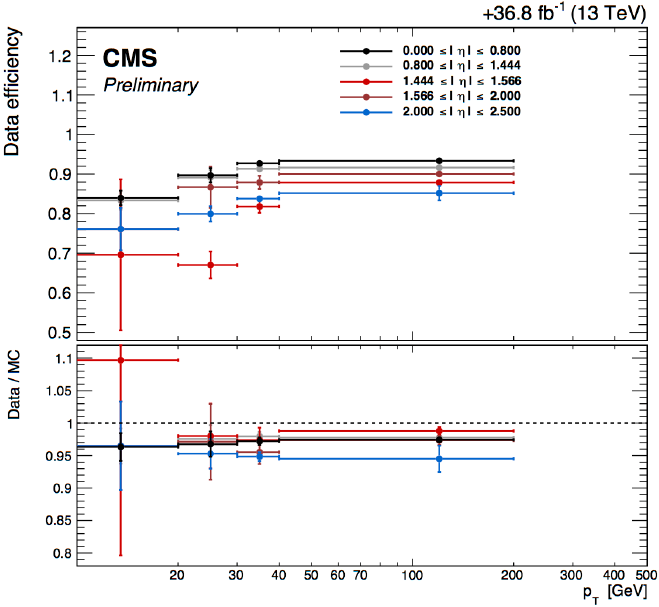
\includegraphics[scale=0.6]{ChapterAnalysis/figs/electron_selection_efficiencies_ingap}}\\
	\subfloat[]{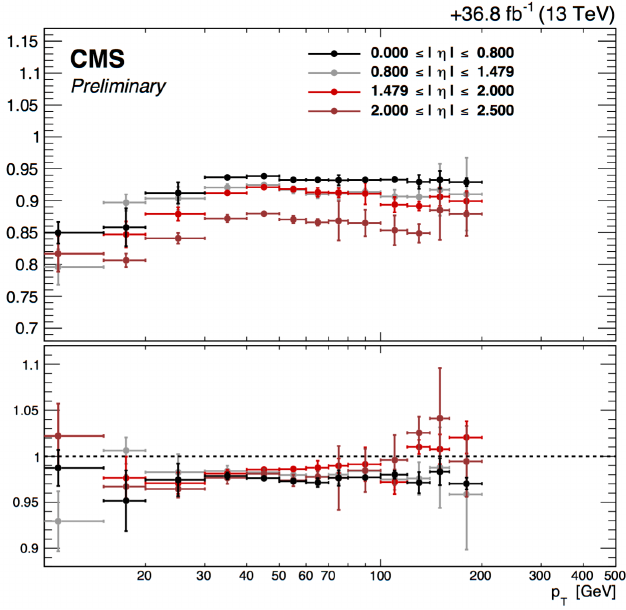
\includegraphics[scale=0.6]{ChapterAnalysis/figs/electron_selection_efficiencies_nongap}}
	\source{CMS COLLABORATION, 2016, p. 18.}
	\label{fig:electron_selection_efficiency}
\end{figure}


\section{Muons}
Further details on muon reconstruction can be found in \cite{bib:CMS-AN-16-328}. Two types of selection are performed. We define \textbf{loose muons} as the muons satisfying $p_{T}>$ 5GeV, $|\eta|<$ 2.4, $d_{xy}<$ 0.5cm and $d_{z}<$ 1cm, where $d_{xy}$ and $d_{z}$ are defined with respect to the primary vertex (PV) and using the \textit{muonBestTrack}. Muons have to be reconstructed by either the \textit{GlobalMuon} or \textit{TrackerMuon} algorithm. Standalone muon tracks reconstructed only in the muon system are rejected. Muons with \textit{muonBestTrackType} == 2 (standalone) are also discarded, even if they are marked as global or tracker muons. Loose muons with $p_{T}<$ 200GeV are considered \textit{tight muons} if they also pass the PF muon ID (note that the naming convention used for these IDs differs from the muon POG naming scheme, in which the "tight ID" used here is called the "loose ID"). Loose muons with $p_{T}>$ 200GeV are considered tight muons if they pass the PF ID or the Tracker High-$p_{T}$ ID, the definition of which is shown in Tab.~\ref{tab:mu_tracker_highpTID_requirements}.

\begin{table}[hbtp]{16cm}
	\caption{The requirements for a muon to pass the tracker high-$p_{T}$ ID. Note that these are equivalent to the Muon POG high-$p_{T}$ ID with the global track requirements removed.}
	\centering
	\begin{tabular}{l|p{9cm}}
		\hline
		Plain-text description     & Technical description\\
		\hline
		Muon station matching      & Muon is matched to segments in at least two muon stations\\
		Good $p_{T}$ measurement   & $p_{T}/\sigma_{p_{T}} < 0.3$\\
		Vertex compatibility (x-y) & $d_{xy} < 2mm$\\
		Vertex compatibility (x)   & $d_{z}<5mm$\\
		Pixel hits                 & At least one pixel hit\\
		Tracker hits               & Hits in at least six tracker layers\\
		\hline
	\end{tabular}
	\source{CMS COLLABORATION, 2016, p. 18.}
	\label{tab:mu_tracker_highpTID_requirements}
\end{table}

An additional "ghost-cleaning" step is performed to deal with situations when a single muon can be incorrectly reconstructed as two or more muons:
\begin{itemize}
	\item Tracker Muons that are not Global Muons are required to be "arbitrated", i.e. associated to the segments in the outer muon detectors;
	\item If two muons are sharing 50$\%$ or more of their segments, the muon with lower quality is removed.
\end{itemize}

Muons are required to be isolated similarly as described for electrons. The pileup contribution subtraction is performed in a different way for muons. A correction $\Delta \beta = \frac{1}{2}(\sum_{PU}^{charged~had.} p_{T})$, that gives an estimate of the energy deposit from neutral particles coming from pileup vertices, is applied. The relative muon isolation is then defined as 

\begin{equation}
RelPFiso = \frac{\sum^{charged~had.} p_{T} + max(\sum^{neutral~had.} E_{T} + \sum^{photon} E_{T} - \Delta \beta, 0)}{p_{T}^{lepton}}
\end{equation}

The muon isolation was optimized in \cite{bib:CMS-AN-15-277} and the working point is chosen to be equal to the one for electrons, that is, RelPFiso$(\Delta R = 0.3)<$ 0.35.

\subsection{Muon Efficiency Measurements}
Muon efficiencies are also measured with the T$\&$P method, which is then performed on $Z \rightarrow \mu\mu$ and $J/\psi \rightarrow \mu\mu$ events in bins of $p_{T}$ and $\eta$. More details on the methodology can be found in \cite{bib:CMS-AN-15-277}. The Z sample is used to measure the muon reconstruction and identification efficiency at high $p_{T}$, and the efficiency of isolation and impact parameter at $p_{T}$. The $J/\psi$ sample is used to measure the reconstruction efficiency at low $p_{T}$ as it benefits from a better purity in such kinematic regime. Events are collected using HLT\_Mu7p5\_Track2\_Jpsi\_v* when probing the reconstruction and identification efficiency in the muon system. For probing the muon tracking efficiency HLT\_Mu7p5\_L2Mu2\_Jpsi\_v* is used.

Muon reconstruction and identification efficiency for $p_{T}>$ 20GeV have been derived by the Muon POG. The probe in this measurement are tracks reconstructed in the inner tracker, and the passing probes are those that are also reconstructed as a global or tracker muon and passing the Muon POG Loose muon identification. For low $p_{T}$ muons $J/\psi$ events have been used, with the same definitions of
"probe" and "passing probe". The systematic uncertainties are estimated by varying the analytical signal and background shape models used to fit the di-muon invariant mass. Details on the procedure can be found in \cite{bib:CMS-AN-15-277}. The efficiency and scale factors used for low $p_{T}$ muons
are the ones derived using single muon prompt-Reco dataset\footnote{These are datasets created by CMS when collecting data. They have the first reconstruction of the events in the collected data.}. The efficiencies in data and in simulation are shown in Fig.~\ref{fig:muon_reco_id_efficiency}.

\begin{figure}[hbtp]{16cm}
	\caption{Muon reconstruction and identification efficiency for $p_{T}<$ 20GeV as a function of $p_{T}$ in the barrel (a) and endcaps (b), and as a function of $\eta$ for $p_{T}>$ 7GeV (c). In the upper panel the cyan (black) error bars show only the statistical uncertainty and the red (violet) ones represent the total uncertainty from MC (data). In the ratio plot of the two efficiencies, the black error bars represent the statistical uncertainty, the orange ones the systematical uncertainty, and the violet ones the total uncertainty.}
	\centering
	\subfloat[]{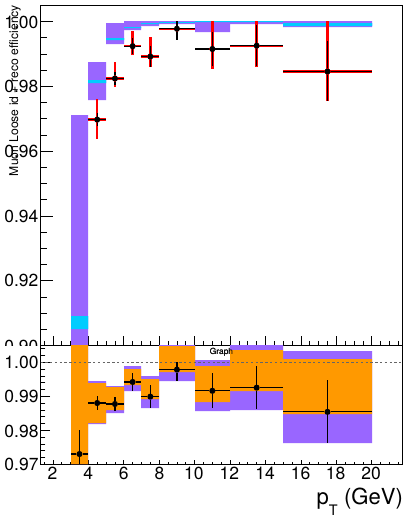
\includegraphics[scale=0.45]{ChapterAnalysis/figs/muon_reco_id_eff_barrel}}
	\quad
	\subfloat[]{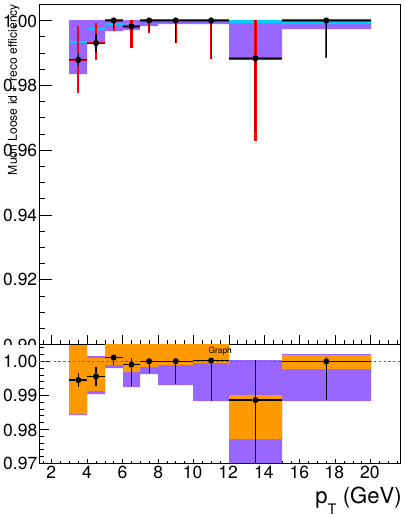
\includegraphics[scale=0.45]{ChapterAnalysis/figs/muon_reco_id_eff_endcap}}
	\quad
	\subfloat[]{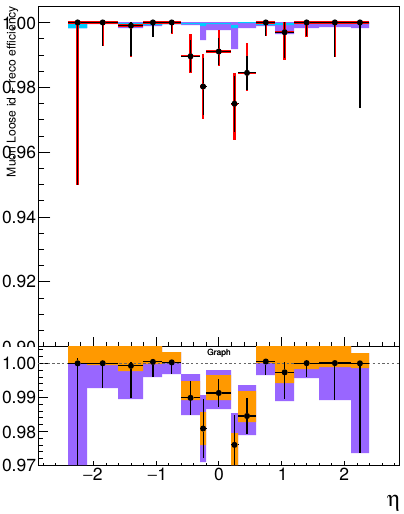
\includegraphics[scale=0.45]{ChapterAnalysis/figs/muon_reco_id_eff_eta}}
	\source{CMS COLLABORATION, 2016, 20.}
	\label{fig:muon_reco_id_efficiency}
\end{figure}

The requirements for the impact parameter is studied using Z events selected with the trigger HLT\_IsoMu20\_v* or HLT\_IsoMu22\_v*. For this measurement, the probe is a muon passing the POG "loose" identification criteria, and it is considered a "passing" probe if it satisfies the $SIP_{3D}$, $d_{xy}$ and $d_{z}$ cuts\footnote{$SIP_{3D} = IP/\sigma_{IP}$ is the significance of the impact parameter (a ratio between the impact parameter in 3D - distance from collision center - and its associated uncertainty), $d_{xy}$ is the distance to the beam in the \textbf{xy} plane and $d_{z}$ is the distance in the \textbf{z} direction to the primary vertex (that is, the collision point).} of this analysis. The results are shown in Fig.~\ref{fig:muon_sip_efficiency}.

\begin{figure}[hbtp]{16cm}
	\caption{Efficiency of the muon impact parameter requirements as a function of $p_{T}$ in the barrel (a) and endcaps (b), and as a function of $\eta$ for $p_{T}>$ 20GeV (c). In the upper panel the cyan (black) error bars show only the statistical uncertainty and the red (violet) ones represent the total uncertainty from MC (data). In the ratio plot the black error bars are for the statistical uncertainty, the orange ones for the systematical uncertainty and the violet ones include both uncertainties.}
	\centering
	\subfloat[]{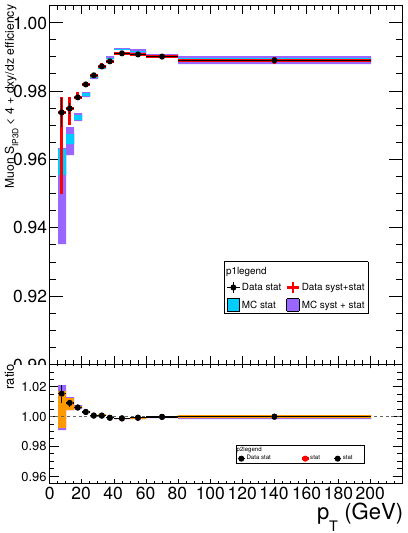
\includegraphics[scale=0.45]{ChapterAnalysis/figs/muon_sip_eff_barrel}}
	\quad
	\subfloat[]{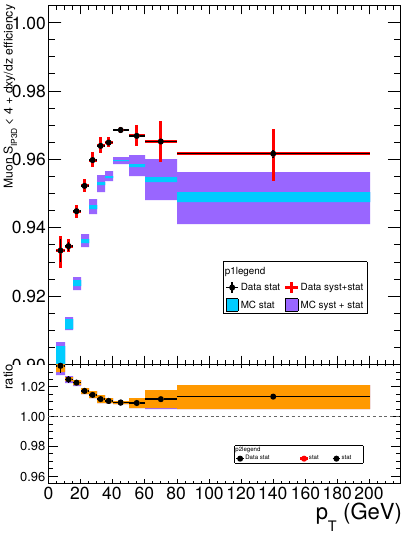
\includegraphics[scale=0.45]{ChapterAnalysis/figs/muon_sip_eff_endcap}}
	\quad
	\subfloat[]{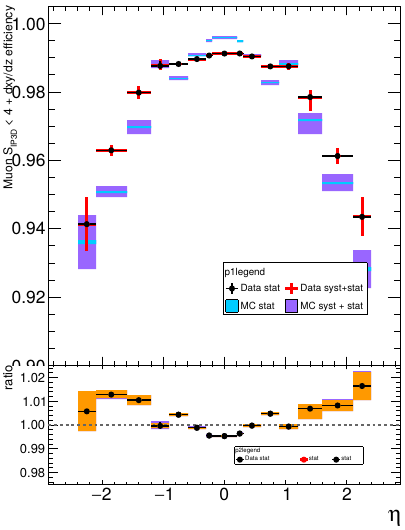
\includegraphics[scale=0.45]{ChapterAnalysis/figs/muon_sip_eff_eta}}
	\source{CMS COLLABORATION, 2016, p. 20.}
	\label{fig:muon_sip_efficiency}
\end{figure}

The muon isolation efficiency is measured using events from the Z decay at any $p_{T}$. The events are selected with the same triggers as for the SIP study. The isolation of the muons are calculated after recovery of the FSR photons and subtracting their contribution from the isolation cone of the muons. More detailed description of the method can be found in \cite{bib:CMS-AN-16-328}. Results are shown in Fig.~\ref{fig:muon_iso_efficiency}.

\begin{figure}[hbtp]{16cm}
	\caption{Efficiency of the muon isolation requirement as a function of $p_{T}$ in the barrel (a) and endcaps (b). In the upper panel the cyan (black) error bars show only the statistical uncertainty and the red (violet) ones represent the total uncertainty from MC (data). In the ratio plot the black error bars are for the statistical uncertainty, the orange ones for the systematical uncertainty and the violet ones for the total uncertainty.}
	\centering
	\subfloat[]{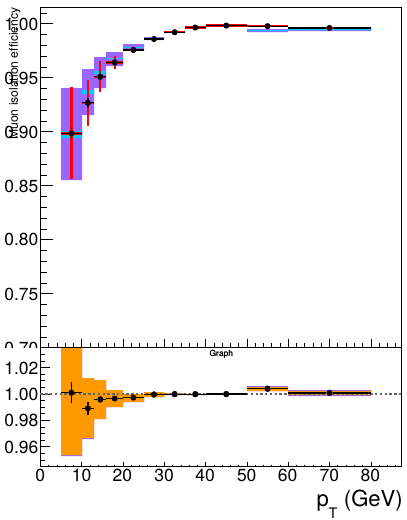
\includegraphics[scale=0.45]{ChapterAnalysis/figs/muon_iso_eff_barrel}}
	\quad
	\subfloat[]{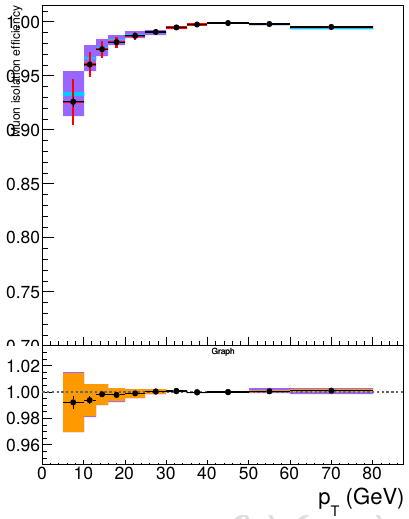
\includegraphics[scale=0.45]{ChapterAnalysis/figs/muon_iso_eff_endcap}}
	\source{CMS COLLABORATION, 2016, p. 21.}
	\label{fig:muon_iso_efficiency}
\end{figure}

The efficiency to reconstruct a muon track in the inner detector is measured using tracks reconstructed only in the muon system. The method for measuring the tracking efficiency is the same as in \cite{bib:CMS-AN-15-215} and the results on 2016 data are briefly discussed here. The efficiency and data-to-simulation scale factors are measured from Z events as a function of $\eta$. The values of data-to-simulation scale factors used are from the ReReco version\footnote{That means a previous reconstructed version of the data collected by CMS have been reprocessed using new settings in the CMS simulation.} of the full dataset collected in 2016. The tracking efficiency in data and in simulation as a function of $\eta$ is shown in Fig.~\ref{fig:muon_tracking_efficiency}.

\begin{figure}[hbtp]{16cm}
	\caption{Tracking efficiency in data and simulation as a function of $\eta$ for muon $p_{T}<$ 10GeV (a) and $p_{T}>$ 10GeV (b) with ReReco data.}
	\centering
	\subfloat[]{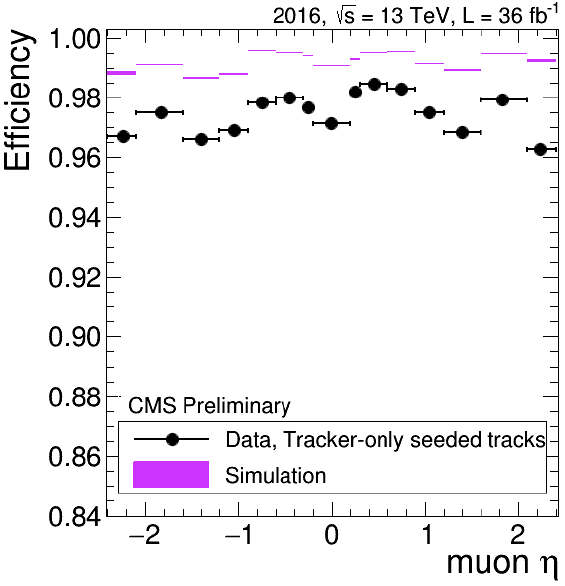
\includegraphics[scale=0.3]{ChapterAnalysis/figs/muon_tracking_eff_ptless10}}
	\quad
	\subfloat[]{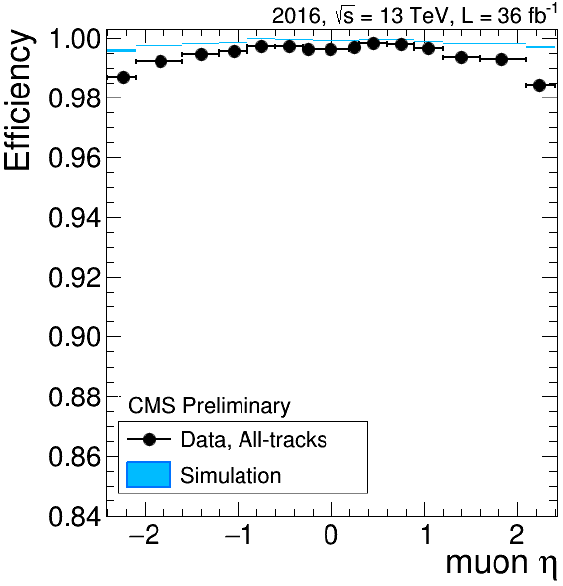
\includegraphics[scale=0.3]{ChapterAnalysis/figs/muon_tracking_eff_ptabove10}}
	\source{CMS COLLABORATION, 2016, p. 22.}
	\label{fig:muon_tracking_efficiency}
\end{figure}

The product of all data-to-simulation scale factors for muon tracking, reconstruction, identification, impact parameter and isolation requirements is used in the analysis.

\section{Photons and FSR Recovery}
The FSR recovery algorithm was considerably simplified with respect to what was done in RunI, while maintaining a similar performance. The selection of FSR photons is now only done per-lepton and no longer depends on any Z mass criteria, which significantly simplifies the building and selection of ZZ candidates. In the association of photons and leptons the rectangular cuts on $\Delta R(\gamma,l)$ and $E_{T,\gamma}$ have been replaced by a cut on $\Delta R(\gamma,l)/E_{T,\gamma}^{2}$.

Starting from the collection of photons provided by the PF algorithm (PF photons), the selection of photons and their association to a lepton proceeds as follows:
\begin{itemize}
	\item[1] The pre-selection of PF photons is done by requiring $p_{T}^{\gamma}>$ 2GeV, $|\eta^{\gamma}|<$ 2.4, and a RelPFiso$(\Delta R=0.3)<$ 1.8. The RelPFiso computation uses a threshold of 0.2GeV on charged hadrons, with a veto cone of 0.0001, and 0.5GeV on neutral hadrons and photons, with a veto cone of 0.01, also including the contribution from pileup vertices (with the same radius and threshold as per-charged isolation);
	\item[2] Supercluster veto: we remove all PF photons that match with any electron passing both the loose ID and SIP cuts. The matching is performed by directly associating the two PF candidates;
	\item[3] Photons are associated to the closest lepton in the event among all those that pass both the loose ID and SIP cuts;
	\item[4] Photons that do not satisfy $\Delta R(\gamma,l)/E_{T,\gamma}^{2}<$ 0.012 and $\Delta R(\gamma,l)<$ 0.5 are discarded;
	\item[5] If more than one photon is associated to the same lepton, we select the one with lowest $\Delta R(\gamma,l)/E_{T,\gamma}^{2}$;
	\item[6] Each selected FSR photon is removed from the isolation sum of all the leptons in the event that pass both the loose ID and SIP cuts. This concerns the photons that are in the isolation cone and outside the isolation veto of said leptons ($\Delta R<$ 0.4 AND $\Delta R>$ 0.01 for muons, and $\Delta R<$ 0.4 AND ($\eta^{SC}<$ 1.479 OR $\Delta R>$ 0.08) for electrons).
\end{itemize}

More details about the photon FSR optimization can be found in \cite{bib:CMS-AN-15-277,bib:CMS-AN-16-442}.


\section{Jets}
Jets are reconstructed through the anti-$k_{T}$ clustering algorithm using PF\footnote{Particle Flow: a set of algorithms developed by the CMS collaboration. It combine the signals coming from every CMS sub-detector in order to reconstruct the particle flow through CMS.} candidates after rejecting the charged hadrons that are associated to a pileup primary vertex. We use a distance parameter $R$ = 0.4. To reduce instrumental background, the loose working point for the jet identification suggested by the JetMET POG is applied. Jets are required to have $p_{T}>$ 30GeV and $|\eta|<$ 4.7 and are cleaned from any tight leptons and FSR photons by a separation criterion of $\Delta R(jet,l/\gamma)>$ 0.4. Since the calorimeter response to particles is not linear, Jet Energy Corrections (JEC) are needed to translate the measured jet energy to the true particle/parton energy. Standard JEC are applied on reconstructed jets, which consist of L1 Pileup, L2 Relative Jet Correction, L3 Absolute Jet Correction for both MC samples and data, and also residual calibration for data. For the purpose of reducing the background coming from $t\bar{t}$ events, the \textit{Combined Secondary Vertex} (CSV) algorithm is used as b-tagging algorithm. It combines information about the SIP, the secondary vertex (SV) and jet kinematics. These variables are combined through a likelihood ratio technique to compute the b-tag discriminator. In this analysis, a jet is considered to be b-tagged if the discriminator \textit{pfCombinedInclusiveSecondaryVertexV2BJetTags} $>$ 0.8484 (i.e. the jet passes the \textit{CSVv2M} "medium" working point). Data-to-simulation scale factors for b-tagging efficiency are provided for this working point for the full dataset as a function of jet $p_{T}$, $\eta$ and flavour. Such scale factors are applied to simulated jets by downgrading (upgrading) the b-tagging status of a fraction of the b-tagged (untagged) jets that have a scale factor smaller (larger) than one \cite{bib:CMS-AN-15-277,bib:CMS-AN-16-442}.

\section{Missing Transverse Energy}
The missing transverse energy (MET), $E_{p_{T}}^{miss}$, of an event
consists of the imbalance in the transverse plane with respect to the beam axis. Since the sum of momentum in the transverse plan must be zero, any imbalance is attributed to undetected particles (such as neutrinos) escaping the CMS detector. Raw $E_{T}^{miss}$ (PFMET) is defined as the magnitude of the negative vectorial sum of all reconstructed PF particles $p_{T}$,

\begin{equation}
\vec{E}_{T}^{miss} = - \sum_{j\epsilon all} \vec{p}_{T,i}
\end{equation}

An alternative definition of MET, which is called Type-I corrected $E_{p_{T}}^{miss}$, takes into account the JEC, correcting the MET for detector inefficiencies and non-linear responses in the calorimeters. The Type-I corrected MET is given by

\begin{equation}
\vec{E}_{T}^{miss} = - \left( \sum_{jets} \vec{p}_{T,jet}^{JEC} + \sum_{i \epsilon uncl.} \vec{p}_{T,i} \right)
\end{equation}

where the contribution of jets ($\vec{p}_{T,jet}^{JEC}$) and the remaining unclustered objects ($\vec{a}_{T,i}$) are accounted separately.

In order to improve signal-to-noise ratio several filters developed in the JETMET POG \cite{bib:CMS-AN-16-442} are used to select the events in this analysis. Such filters are presented in Tab.~\ref{tab:jetmet_filters}.

\begin{table}[hbtp]{16cm}
	\caption{Filters from JETMET POG used to improve signal-to-noise ratio.}
	\centering
	\begin{tabular}{p{6cm}|p{9cm}}
		\hline
		Filter & Description\\
		\hline
		HBHENoiseFilter \hspace{3cm} HBHENoiseIsoFilter & remove noisy events from the HCAL, where the HBHE scintillator produces anomalous signals with pulse shapes and pixel multiplicities discrepant from those from a clean signal\\
		\hline
		EcalDeadCellTriggerPrimitiveFilter & removes events with non-functioning ECAL data links, comparing the sum of energy deposited in each supercluster cell to the energy saturation of the trigger primitive\\
		\hline
		goodVertices & filter events with noisy vertex reconstruction (due to pileup effects) by requiring the reconstruction of at least one good vertex full filling the following criteria: high number of degree of freedom ($NPV>$ 4), collisions restricted along the z−axis ($zPV<$ 24cm) and small radius of the PV ($rPV<$ 2cm)\\
		\hline
		eeBadScFilter & removes events with noisy ECAL endcap superclusters\\
		\hline
		globalTightHalo2016Filter & removes events with enhanced MET from beam-halo particles which are in time with the beam\\
		\hline
		BadPFMuonFilter \hspace{3cm} BadChargedCandidateFilter & remove events with mis-reconstructed muon and charged hadron PF candidates\\
		\hline
	\end{tabular}
	\source{CMS COLLABORATION, 2016, p. 24. Adapted by the author.}
	\label{tab:jetmet_filters}
\end{table}


%%==========================================================================
\chapter{Event Selection}
\label{sec:event_selection}
%%==========================================================================
The selections performed in this analysis are designed to reconstruct a final state with four charged leptons ($4\mu$, $4e$ or $2e2\mu$) and MET. The four-lepton system must satisfy the SM Higgs selections described in \cite{bib:CMS-AN-16-442}. 

\section{Preselection}
The events must have fired at least one of the HLT paths presented in Chapter~\ref{sec:datasets}. They are also required to pass the MET filters described in Chapter~\ref{sec:physics_objects_selections}.

\section{Selection of the ZZ System}
The events with four lepton candidates are selected from what is called \textit{selected leptons}, which are the tight leptons defined in Chapter~\ref{sec:physics_objects_selections}. Such leptons have $SIP_{3D} <$ 4 as a vertex constraint and isolation cuts, where the FSR photons are removed from the isolation cone. A lepton cross cleaning, which discards leptons with $\Delta R \leq$ 0.05 from each other, is applied.

The building of a ZZ system from four candidate leptons proceeds according to the following sequential steps:
\begin{itemize}
	\item [1] \textbf{Z candidates}: are built from a pair of selected leptons of opposite charge and same flavor ($e^{+}e^{-}$, $\mu^{+}\mu^{-}$), having invariant mass satisfying $12 < m_{ll(\gamma)}<$ 120GeV, where the Z candidate mass takes into account (if any) a selected FSR photon;
	\item [2] \textbf{ZZ candidates}: are built from a pair of Z candidates which do not have common leptons (non-overlapping). The Z with closest $m_{ll(\gamma)}$ to the nominal Z boson mass is denoted as $Z_{1}$ and the second one is the $Z_{2}$. The built ZZ system must satisfy the following requirements:
	\begin{itemize}
		\item \textbf{Ghost removal}: any two leptons must have $\Delta R(\eta,\phi) > 0.02$;
		\item \textbf{Lepton $p_{T}$}: at least two out of the four leptons must have $p^{i}_{T} > 10$ and $p^{i}_{T} > 20$ GeV;
		\item \textbf{QCD suppression}: all opposite-sign lepton pair that can be built out of the four leptons (regardless of lepton flavor) must satisfy $m_{ll} > 4$ GeV. Here, the selected FSR photons are not included in the mass computation, since QCD-induced low mass dilepton (e.g. $J/\Psi$) may have photons nearby (e.g. from $\pi^{0}$);
		\item \textbf{$Z_{1}$ mass}: $m_{Z_{1}} > 40$ GeV;
		\item \textbf{Smart cut}: defining $Z_{a}$ and $Z_{b}$ as the mass-sorted alternative pairing Z candidate ($Z_{a}$ being the closest one to the nominal Z mass), require NOT($|m_{Z_{a}}-m_{Z}| < |m_{Z_{1}}-m_{Z}|$ AND $m_{Z_{b}} < 12$). Selected FSR photons are included in the $m_{Z}$'s computation. This cut discards 4$\mu$ and 4e candidates which have the alternative pairing similar to an on-shell Z + a low-mass pair $l^{+}l^{-}$;
		\item \textbf{Four-lepton invariant mass}: $m_{4l} > 70$ GeV;
		\item \textbf{Choice of the best ZZ candidate}: if more than one ZZ candidate survives the previous selections, the one with the highest four leptons $p_{T}$ scalar sum is chosen.
	\end{itemize}
	\item [3] \textbf{SM Higgs selection}: events containing at least one ZZ system satisfying all the previous selections are then used to tag the Higgs decaying into four lepton final state, as it is done for the SM Higgs analysis \cite{bib:CMS-AN-16-442};
	\item [4] \textbf{Signal region (SR)}: in order to enhance the presence of VBF events over the other SM Higgs production modes and the SM backgrounds, additional cuts are applied as discussed in the next section.
\end{itemize}

\section{VBF Signal Region (VBF-SR)}
\label{subsec:vbf_sr}
In order to optimize the analysis for the VBF production mode few additional requirements are imposed to the events selected after the steps described above (until step 3). These additional selections are:
\begin{itemize}
	\item \textbf{Number of jets}: events must have,
	\begin{itemize}
		\item EITHER, two or three jets from which at most one b-tagged jet;
		\item OR, more than three jets with no b-tagged jet;
	\end{itemize}
	\item \textbf{Four-lepton invariant mass}: events must have $118 \leq m_{4l} \leq 130$ GeV since the significant fraction of VBF yields is contained within that range. This $m_{4l}$ range is equal to the SM Higgs signal region adopted by CMS collaboration \cite{bib:JHEP11_047_2017}.
\end{itemize} 

Note that these VBF-SR requirements are similar to the standard ones used by CMS Collaboration defining the VBF category \cite{bib:JPhys-447-1-2013,bib:CMS-AN-16-442}. The difference, since the Artificial Neural Networks (ANNs) are the discriminants of interest in this analysis, is that the CMS MELA discriminant for VBF 2-jets category (denoted by $D_{qqH,2j}^{MELA}$ in the text) is not used to categorize events. The Tab.~\ref{tab:sm_higgs_yields} and Tab.~\ref{tab:vbf_sr_yields} show the yields for each process after the SM Higgs and VBF-SR selections, respectively. The Fig.~\ref{fig:control_plots} shows $m_{4l}$ distributions for such events. Note that those tables don't include yet the contribution coming from the reducible background (Z+X) that will be discussed in detail in Chapter~\ref{sec:zx_estimation}.

\begin{table}[hbtp]{16cm}
	\footnotesize
	\caption{Number of expected events for background and signal, with statistical uncertainty reported, and number of observed events after the SM Higgs selections.}
	\centering
	\begin{tabular}{c|c|c|c|c}
		\hline
		\rowcolor{light_gray}
		Process                     & 4$\mu$          & 4e              & 2e2$\mu$        & 4l\\
		ggH                         &  19.34$\pm$0.14 &  11.02$\pm$0.11 &  25.99$\pm$0.16 &   56.35$\pm$0.24\\
		VH                          &   1.45$\pm$0.01 &   0.92$\pm$0.01 &   2.14$\pm$0.01 &    4.51$\pm$0.01\\
		ttH                         &   0.36$\pm$0.00 &   0.23$\pm$0.00 &   0.48$\pm$0.00 &    1.07$\pm$0.01\\
		qqZZ+ZZJJ                   & 387.01$\pm$1.67 & 234.64$\pm$1.31 & 538.35$\pm$1.97 & 1160.00$\pm$2.90\\
		ggZZ                        &  65.81$\pm$0.09 &  43.85$\pm$0.08 & 102.32$\pm$0.13 &  211.98$\pm$0.18\\
		\hline
		$\sum$ backgrounds          & 473.97$\pm$1.68 & 290.66$\pm$1.31 & 669.29$\pm$1.98 & 1433.91$\pm$2.91\\
		\hline
		qqH (signal $m_{H}=125GeV$) &   1.86$\pm$0.01 &   1.10$\pm$0.01 &   2.53$\pm$0.01 &    5.49$\pm$0.02\\
		\hline
		Total expected              & 475.83$\pm$1.68 & 291.76$\pm$1.74 & 671.81$\pm$1.98 & 1433.91$\pm$2.92\\
		\hline
		Observed                    & 503             & 287             & 669             & 1459\\
		\hline
	\end{tabular}
	\source{The author, 2018.}	
	\label{tab:sm_higgs_yields}
\end{table}

\begin{table}[hbtp]{16cm}
	\footnotesize
	\caption{Number of expected events for background and signal and number of observed events after the VBF-SR selections.}
	\centering
	\begin{tabular}{c|c|c|c|c}
		\hline
		\rowcolor{light_gray}
		Process                     & 4$\mu$        & 4e            & 2e2$\mu$      & 4l\\
		ggH                         & 2.46$\pm$0.05 & 1.28$\pm$0.04 & 3.10$\pm$0.06 & 6.84$\pm$0.08\\
		VH                          & 0.34$\pm$0.00 & 0.20$\pm$0.00 & 0.46$\pm$0.00 & 1.00$\pm$0.01\\
		ttH                         & 0.05$\pm$0.00 & 0.03$\pm$0.00 & 0.06$\pm$0.00 & 0.14$\pm$0.00\\
		qqZZ+ZZJJ                   & 0.67$\pm$0.07 & 0.36$\pm$0.05 & 0.74$\pm$0.07 & 1.77$\pm$0.10\\
		ggZZ                        & 0.05$\pm$0.00 & 0.03$\pm$0.00 & 0.06$\pm$0.00 & 0.14$\pm$0.01\\
		\hline
		$\sum$ backgrounds          & 3.57$\pm$0.08 & 1.90$\pm$0.06 & 4.42$\pm$0.09 &  9.89$\pm$0.13\\
		\hline
		qqH (signal $m_{H}=125GeV$) & 1.05$\pm$0.01 & 0.58$\pm$0.01 & 1.39$\pm$0.01 &  3.02$\pm$0.02\\
		\hline
		Total expected              & 4.62$\pm$0.08 & 2.48$\pm$0.06 & 5.81$\pm$0.09 & 12.91$\pm$0.13\\
		\hline
		Observed                    & 5             & 2             & 10            & 17\\
		\hline
	\end{tabular}
	\source{The author, 2018.}	
	\label{tab:vbf_sr_yields}
\end{table}

\begin{figure}[hbtp]{16cm}
	\caption{Control plots of four-lepton invariant mass for: (a) events passing the SM Higgs selection, (b) events in the $m_{4l} = [118,130]$ GeV range and (c) events in the VBF signal region.}
	\centering
	\subfloat[]{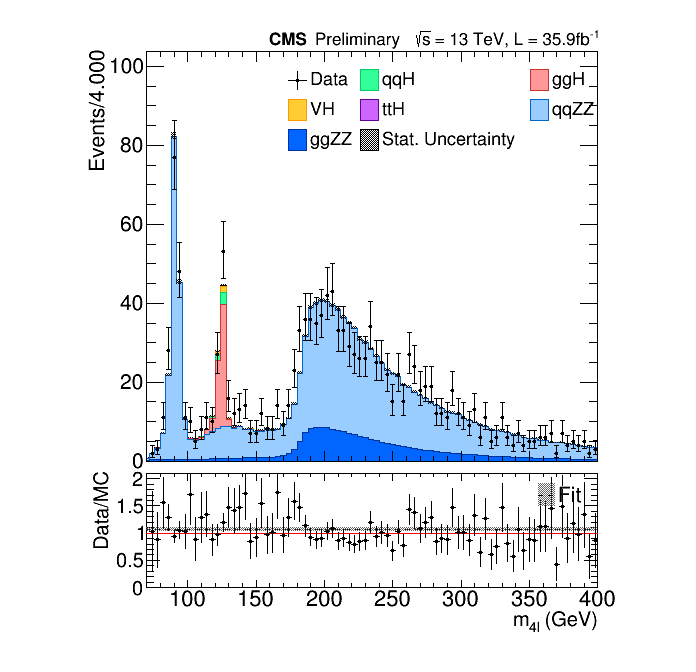
\includegraphics[scale=0.4,trim={2cm 0cm 2cm 0cm},clip]{ChapterAnalysis/figs/histo_mass4l_full_range}}
	\subfloat[]{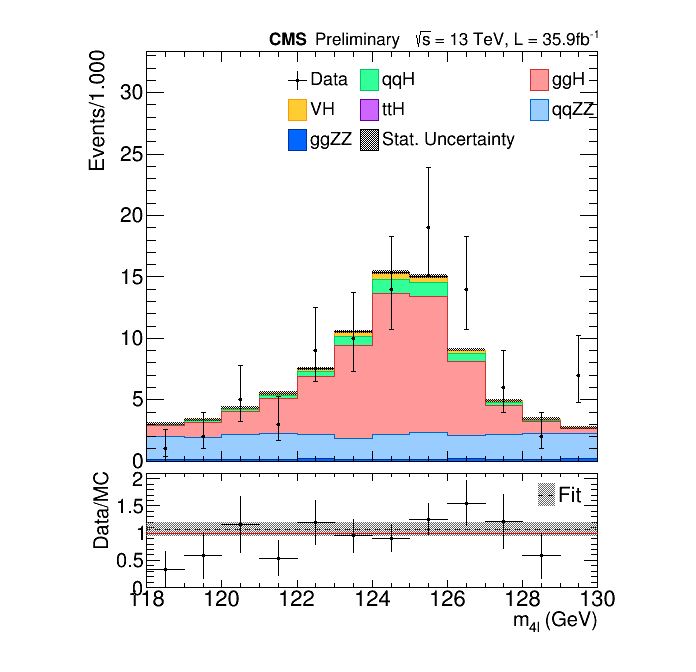
\includegraphics[scale=0.4,trim={2cm 0cm 2cm 0cm},clip]{ChapterAnalysis/figs/histo_mass4l_higgs_sr}}\\
	\subfloat[]{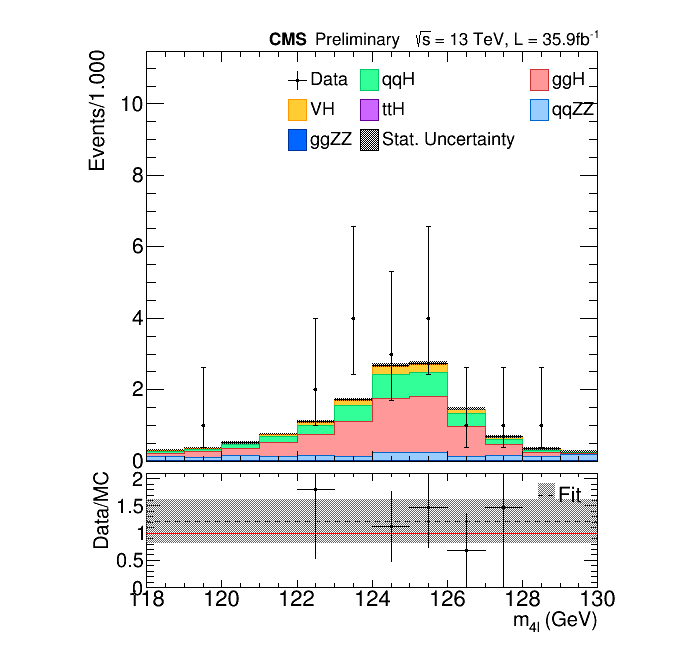
\includegraphics[scale=0.4,trim={2cm 0cm 2cm 0cm},clip]{ChapterAnalysis/figs/histo_mass4l_vbf_sr}}
	\source{The author, 2018.}	
	\label{fig:control_plots}		
\end{figure}


%%==========================================================================
\chapter{Neural Networks}
\label{sec:neural_networks}
%%==========================================================================
As shown on previous sections the Higgs VBF signal is quite small compared to its main background (the main Higgs production mode $ggH$). In order to enhance the signal efficiency this analysis was meant to be based on Artificial Neural Networks (ANNs) instead of applying rectangular cuts as usual. 

An ANN is an interconnected assembly of small processing units usually called neurons (also activations or nodes). Each of these units performs individual operations and communicates between themselves their results. Such a design was motivated by analogy with
the brain, which can be thought as a highly complex, nonlinear and parallel computer. It is estimated that the human brain has 100 billion neurons and each one of them typically receives thousands of connections from other neurons. The inter-neuron connections are mediated by electrochemical junctions, the so called synapses, which happens on branches of the cell called dendrites. These thousand of signals are then combined and depending of the result of this combination the neuron outputs a signal to its neighborhood \cite{bib:SimonHaykin,bib:KevinGurney}.

Similar to the brain, ANNs have the capability to learn from patterns and generalize the modeling of such patterns. This generalization means the possibility to correct identification of a pattern that was not seen before by the ANN during the learning process. The neurons contain a function which can receives also several arguments (inputs) and combine them into a single output value (Fig.~\ref{fig:nn_neuron_example}). There are several types of functions that can be used in the neurons and the choice of the best one might depend on each type of problem. The way the neurons are assembled also can be done in several ways, such that there are different architecture for the connections of the neurons. But a typical and well representative ANN architecture can be seen in Fig.~\ref{fig:neuron_and_dnn}. This kind of ANN is usually called Deep Neural Network (DNN) due to its many layers. Such ANN has shown capability to learn very complex tasks and its success comes from relatively recent improvements in the Machine Learning (ML) field \cite{bib:GlorotAndBendio2010,bib:NairAndHinton2010,bib:Zeiler_et_al2013}.

\begin{figure}[hbtp]{16cm}
	\caption{(a) Graphical representation of a neuron. Each input \textit{$x_i$} (from user or from the hidden neurons) is weighted by \textit{$w_i$} and summed to a bias \textit{b}. The sum is passed to a function (the activation function - neuron type) which outputs a vector of values (one for each input). (b) Graphical representation of a ANN with three hidden layers. In this type of ANN the outputs of all neurons from a previous layer are fed into the neurons of a next layer.}
	\centering
	\subfloat[]{
		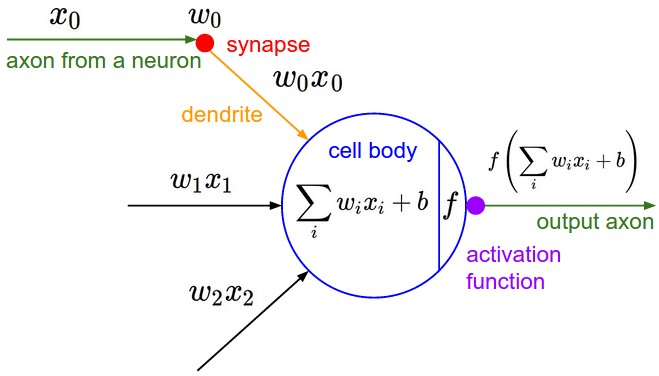
\includegraphics[width=0.56\textwidth]{ChapterAnalysis/figs/nn_neuron_example}
		\label{fig:nn_neuron_example}
	}
	\quad
	\quad
	\quad
	\subfloat[]{
		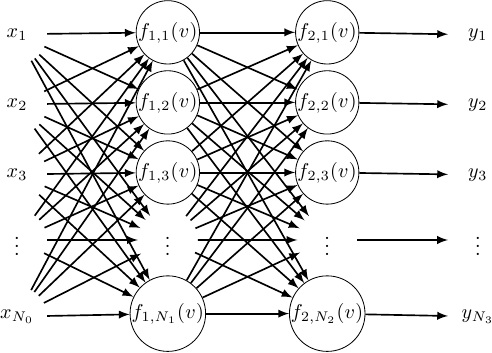
\includegraphics[width=0.62\textwidth]{ChapterAnalysis/figs/dnn_example}
		\label{fig:dnn_example}
	}
	\source{JORDAN, 2018.}	
	\label{fig:neuron_and_dnn}
\end{figure}

Nowadays there are many different flavors of ANNs: Fully Connected Neural Networks (FC-NNs), Convolutional Neural Networks (CNNs), Long Short Term Memory Neural Networks (LSTM-NNs), etc \cite{bib:SimonHaykin}. In principle any of these types of ANNs can be used in any application but each one of them has some particular structure and workflow that benefits differently each application. In the present analysis the FC-NN was chosen. In a fully connected neural network the outputs from all the neurons in a previous layer are passed to all neurons in the next layer and this process happens across the entire ANN in a sequential way (Fig.~\ref{fig:dnn_example}).

\section{The Learning Process}
The way ANNs can be trained allows one to classify the learning process basically in two types: unsupervised and supervised. The former stands for the case when one doesn't know if a given dataset contains some pattern, in other words, if it is not possible to label the objects (read signal/background events) in the dataset. The ANN can be still trained to find out possible patterns existing in the dataset. The supervised procedure is the opposite situation in which one knows that the dataset contains patterns and such patterns are known. The ANN is then trained to correctly assign a given label to a given example. The labels can arbitrarily be chosen and usually for classification task of two classes one uses 0 or 1 for labeling the examples. In order to verify the performance of labels assignment there is a function, usually called \textit{loss} (or cost/risk), which measures the error between the ANN response and what is expected \cite{bib:SimonHaykin}. The output of the \textit{loss} function is the main input used to modify the ANN parameters in order to evolve the modeling of the data. The modification in the ANN parameters (Fig.~\ref{fig:nn_neuron_example}) is done by an algorithm called \textit{back-propagation} which consists basically of an application of the chain rule for partial derivatives.

Exemplifying such process, let's assume a neuron $j$ in a intermediate layer of a neural network. Calling $w_{ji}$ as the weight assigned by that neuron $j$ to an input $y_{i}(n)$ at a given iteration $n$, then such neuron produces a \textit{local field} given by

\begin{equation}
v_{j}(n) = \sum_{i=1}^{m} w_{ji}(n)y_{i}(n) + b_{j}(n)
\label{neuron_local_field}
\end{equation}

in which $m$ stands for the total number of inputs received by the neuron and $b_{j}(n)$ is the so called bias (which is just one value per neuron). This \textit{local field} is then given as an argument to an activation function (represented by $\mathit{f}$ in Fig.~\ref{fig:neuron_and_dnn}) which produces the \textit{signal function} $y_{j}(n)$ of the neuron $j$ at iteration $n$,

\begin{equation}
y_{j}(n) = \mathit{f}[v_{j}(n)]
\end{equation}

It is possible to compute an instantaneous error for the neuron $j$ (Eq.~\ref{eq:instant_error}) using its \textit{signal error} $e_{j}(n)$ which is defined as the difference between the neuron \textit{signal function} $y_{j}(n)$ (its output after the activation function) and the expected \textit{response} $d_{j}(n)$. Note that, the expected response $d_{j}(n)$ can be the label identifying a training example - for neurons in the output layer - or an actual response that a hidden neuron - in the intermediate layers - should have based on the example label. The Eq.~\ref{eq:instant_error} is the core of the so called \textit{loss} or \textit{empirical risk} and it is an example of \textit{loss} function used here in order to exemplify the ANN learning process but, be aware that there are other types. Summarizing, the processes described so far can be graphically represented as shown in Fig.~\ref{fig:neuronj_signal_flow}.

\begin{equation}
\label{eq:instant_error}
\mathcal{E}(n) = \frac{1}{2} e_{j}^{2}(n), ~~\mathrm{with}~~ e_{j}(n) = d_{j}(n) - y_{j}(n)
\end{equation}

\begin{figure}[hbtp]{16cm}
	\caption{The flow of signal through the neuron $j$ up to its instantaneous error $e_{j}$.}
	\centering
	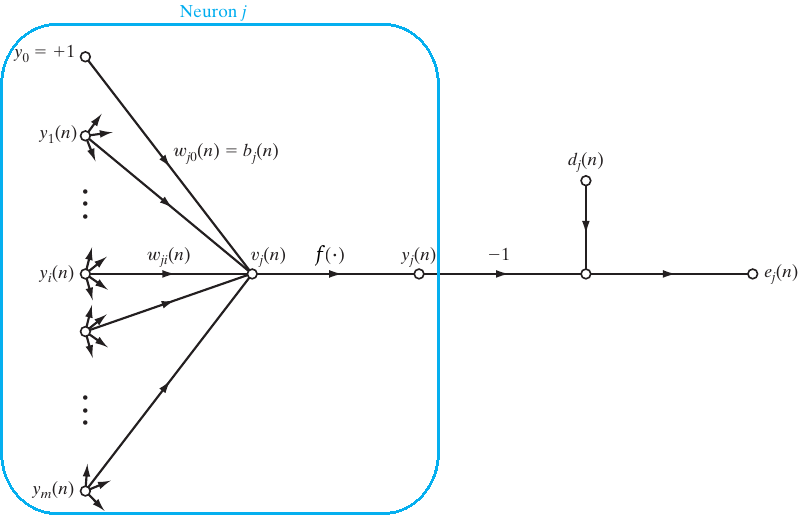
\includegraphics[scale=0.5]{ChapterAnalysis/figs/neuronj_signal_flow}
	\source{HAYKIN, 2009, p. 129. Adapted by the author.}
	\label{fig:neuronj_signal_flow}
\end{figure}

Now, taking the partial derivative of the \textit{loss} by application of the chain rule one gets,

\begin{equation}
\frac{\partial \mathcal{E}(n)}{\partial w_{ji}} = \frac{\partial \mathcal{E}(n)}{\partial e_{j}(n)} ~ \frac{\partial e_{j}(n)}{\partial y_{j}(n)} ~ \frac{\partial y_{j}(n)}{\partial v_{j}(n)} ~ \frac{\partial v_{j}(n)}{\partial w_{ji}(n)}.
\end{equation}

and replacing the derivatives accordingly like so,

\begin{equation}
\frac{\partial \mathcal{E}(n)}{\partial e_{j}(n)} = e_{j}(n)
\end{equation}

\begin{equation}
\label{eq:signal_error_partial}
\frac{\partial e_{j}(n)}{\partial y_{j}(n)} = -1
\end{equation}

\begin{equation}
\frac{\partial y_{j}(n)}{\partial v_{j}(n)} = \mathit{f}'[v_{j}(n)]
\end{equation}

\begin{equation}
\frac{\partial v_{j}(n)}{\partial w_{ji}(n)} = y_{i}(n)
\end{equation}

one reaches to

\begin{equation}
\label{eq:loss_partial}
\frac{\partial \mathcal{E}(n)}{\partial w_{ji}} = -e_{j}(n) ~ \mathit{f}'[v_{j}(n)] ~ y_{i}(n).
\end{equation}

Finally, the correction applied to the weights $w_{ji}$ is given by the \textit{delta rule} as

\begin{equation}
\label{eq:error_correction}
\Delta w_{ji}(n) = - \eta \frac{\partial \mathcal{E}(n)}{\partial w_{ji}}
\end{equation}

where the signal "-" accounts for the descending gradient in the weights space (that is, it seeks for a direction in which the weight change leads to decreasing of $\mathcal{E}(n)$). The $\eta$ term is the so called \textit{learning rate} of the back-propagation algorithm. The Eq.~\ref{eq:error_correction} is the core of the synaptics ($w_{ji}$) update within the neural network. Replacing the Eq.~\ref{eq:loss_partial} into Eq.~\ref{eq:error_correction} yields

\begin{equation}
\label{eq:error_correction_simplified}
\Delta w_{ji}(n) = \eta ~ \delta_{j}(n) ~ y_{i}(n), ~~\mathrm{with}~~\delta_{j}(n) = \frac{\partial \mathcal{E}(n)}{\partial v_{j}(n)}
\end{equation}

The term $\delta_{j}(n)$ is the \textit{local gradient}. From this point there are two situations now:
\begin{itemize}
\item [1] When the neuron is located in the output layer: in such case that neuron is supplied by the labels classifying the examples (which is its \textit{expected response} $v_{j}$) and thus, by Eq.~\ref{eq:instant_error}, one has the error and can compute the \textit{local gradient} $\delta_{j}(n)$;
\item [2] When the neuron is in a hidden layer some complications arise but still Eq.~\ref{eq:error_correction} holds. The Fig.~\ref{fig:hidden_neuronj_signal_flow} showns a scheme of the signal flow in this case. According to Eq.~\ref{eq:error_correction_simplified} and Eq.~\ref{eq:signal_error_partial} it is possible to redefine the \textit{local gradient} for a hidden neuron $j$ as

\end{itemize}
\begin{figure}[hbtp]{16cm}
	\caption{The flow of signal through a hidden neuron $j$ up to its \textit{signal function} $y_{j}(n)$ which is forwarded as an input to an neuron $k$ in an output layer. Note that, the \textit{activation function} can now be different between the layers and they are represented as $f_{j}$ and $f_{k}$ for the neurons $j$ and $k$, respectively.}
	\centering
	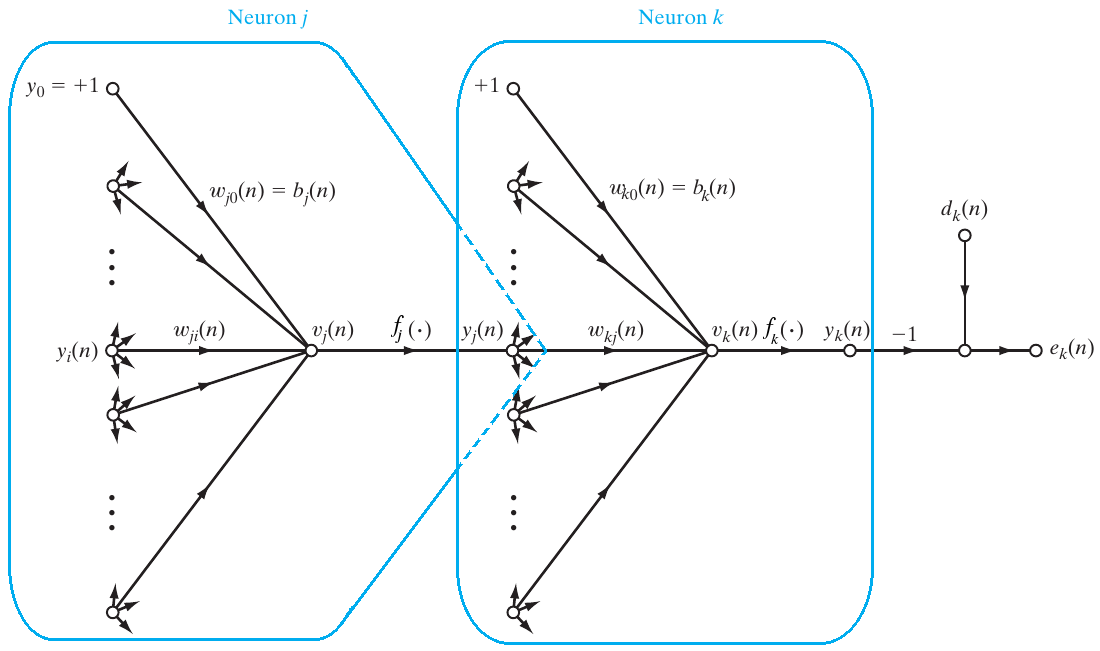
\includegraphics[scale=0.4]{ChapterAnalysis/figs/hidden_neuronj_signal_flow}
	\source{HAYKIN, 2009, p. 132. Adapted by the author.}	
	\label{fig:hidden_neuronj_signal_flow}
\end{figure}

\begin{equation}
\label{eq:local_gradient_hidden}
\delta_{j}(n) = - \frac{\partial \mathcal{E}(n)}{\partial y_{j}(n)} ~ \frac{\partial y_{j}(n)}{\partial v_{j}(n)} = - \frac{\partial \mathcal{E}(n)}{\partial y_{j}(n)} ~ \mathit{f}'[v_{j}(n)].
\end{equation}

From Eq.~\ref{eq:instant_error} and Fig.~\ref{fig:hidden_neuronj_signal_flow} it is clear that $\mathcal{E}(n) = (1/2) \sum_{(k~\epsilon~C)} e_{k}^{2}(n)$. Differentiating this expression with respect to $y_{j}(n)$ one has

\begin{equation}
\label{eq:loss_partial_hidden_neuron}
\frac{\partial \mathcal{E}(n)}{\partial y_{j}(n)} = \sum_{k~\epsilon~C} e_{k}(n) ~ \frac{\partial e_{k}(n)}{\partial y_{j}(n)} \equiv \sum_{k~\epsilon~C} e_{k}(n) ~ \frac{\partial e_{k}(n)}{\partial v_{k}(n)} ~ \frac{\partial v_{k}(n)}{\partial y_{j}(n)}
\end{equation}

Now, from Fig.~\ref{fig:hidden_neuronj_signal_flow} and the previous discussions one sees that,

\begin{eqnarray}
e_{k}(n) &=& d_{k}(n) - y_{k}(n) \equiv d_{k}(n) - \mathit{f}_{k}'[v_{k}(n)] \\
\label{eq:ek_partial}
\frac{\partial e_{k}(n)}{\partial v_{k}(n)} &=& -\mathit{f}_{k}'[v_{k}(n)]\\
v_{k}(n) &=& \sum_{j=1}^{m} w_{kj}(n) y_{j}(n) + b_{k}(n)\\
\label{eq:vk_partial}
\frac{\partial v_{k}(n)}{\partial y_{i}(n)} &=& w_{kj}(n)
\end{eqnarray}

and, using Eq(s).~\ref{eq:ek_partial} and \ref{eq:vk_partial} into \ref{eq:loss_partial_hidden_neuron} one has

\begin{eqnarray}
\label{eq:dedj_hidden}
\nonumber
\frac{\partial \mathcal{E}(n)}{\partial y_{j}(n)} &=& - \sum_{k~\epsilon~C} e_{k}(n) ~ \mathit{f}_{k}'[v_{k}(n)] ~ w_{kj}(n)\\
                                                  &=& - \sum_{k~\epsilon~C} \delta_{k}(n) ~ w_{kj}(n)
\end{eqnarray}

where the definition of \textit{local gradient} has been used. Finally, using Eq.~\ref{eq:dedj_hidden} in \ref{eq:local_gradient_hidden} one finds that the \textit{back-propagation} formula for the hidden neuron $j$ is

\begin{equation}
\label{eq:local_gradient_hidden_final}
\delta_{j}(n) = \mathit{f}_{j}'[v_{j}(n)] ~ \sum_{k~\epsilon~C} \delta_{k}(n) ~ w_{kj},~~\mathrm{neuron}~j~\mathrm{is~hidden}.
\end{equation}

Note that, the sum in Eq.~\ref{eq:local_gradient_hidden_final} is over all the neurons in the output layer. Also note that, $e_{k}(n)$ can be extended to internal layers, such that, it will correspond to the signal errors coming from neurons in the forward hidden layers.


\section{Developing and Training the Neural Networks}
\label{sec:developing_training_neural_networks}
In this analysis the base software used to build up and train the ANNs
is Keras \cite{bib:KerasWebPage}. Keras is a widely used and powerful set of python libraries that allows one to quickly create any type of known ANN. It contains sets of modules that simplify much of the coding needed by the user. Keras has recently been integrated into TMVA \cite{bib:JPhysConfSer_898_072046_2017} and the user has the flexibility to either prepare a C++ code version or to transfer a python version to TMVA which plugs it into Keras. Note however that in the beginning of this analysis that wasn't available and an entire Keras-python framework was developed to make the studies. Using recent version of TMVA cross-checks were made comparing the results got by Keras-python and Keras-TMVA, and the results are in agreement.

\section{Preparation of the Datasets}
\label{subsec:datasets_preparation}
The Neural Networks have been trained using the simulated samples described in Chapter~\ref{sec:datasets} and only with the events passing the selections defining the VBF-SR. As it will be discussed later the variables used into the final ANNs are the leptons and jets three-momentum (that is, $p_{T}$, $\eta$ and $\phi$). The distribution of such variables, for both MC and Data, is shown in Fig.~\ref{fig:ann_input_variables} as a cross-check of the variables shape and Data-MC agreement (the low binning has been chosen due to the low statistic available for Data at the VBF-SR). The Z+X background on those pictures is derived via a stablished CMS data-driven method, which is described in Chapter~\ref{sec:zx_estimation}.

\begin{figure}[hbtp]{16cm}
	\caption{Monte Carlo and Data distribution of the variables used as inputs to train the ANNs in this analysis.}
	\centering
	\subfloat[]{
		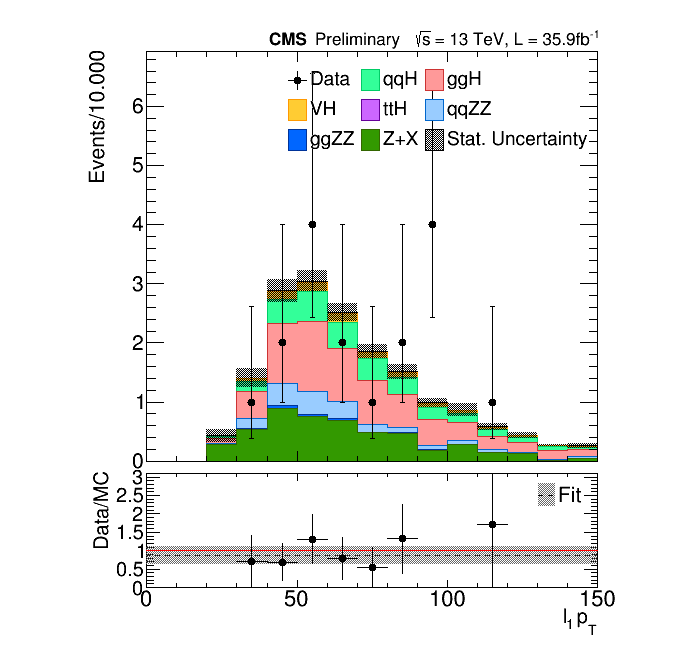
\includegraphics[scale=0.23,trim={2cm 1cm 2cm 1cm},clip]{ChapterAnalysis/figs/vbf_l1_pt}
	}
	\subfloat[]{
		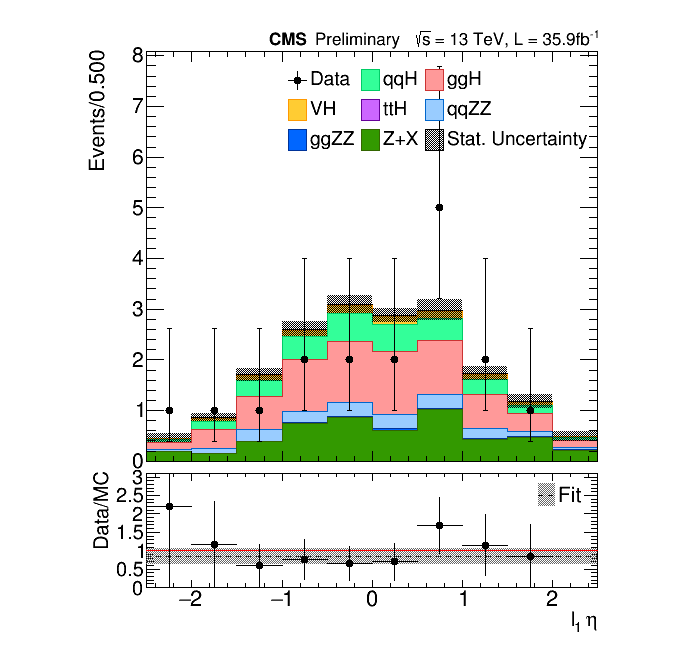
\includegraphics[scale=0.23,trim={2cm 1cm 2cm 1cm},clip]{ChapterAnalysis/figs/vbf_l1_eta}
	}
	\subfloat[]{
		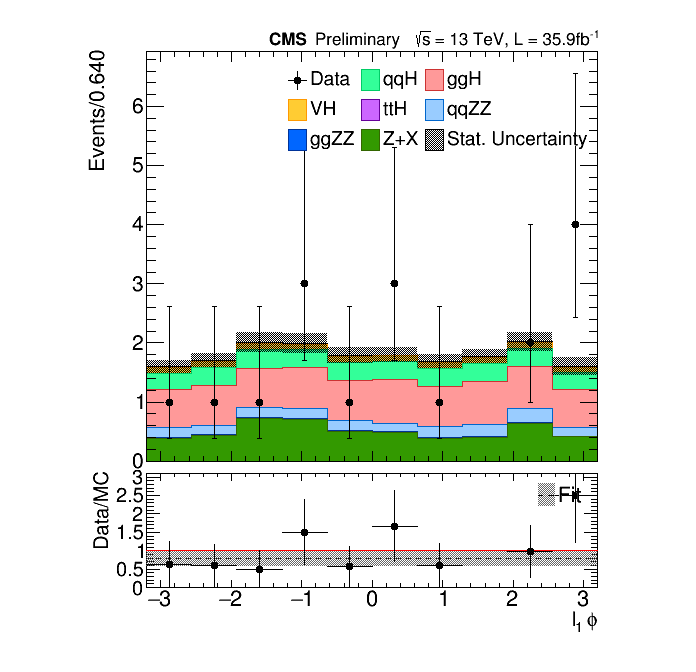
\includegraphics[scale=0.23,trim={2cm 1cm 2cm 1cm},clip]{ChapterAnalysis/figs/vbf_l1_phi}
	}\\
	\subfloat[]{
		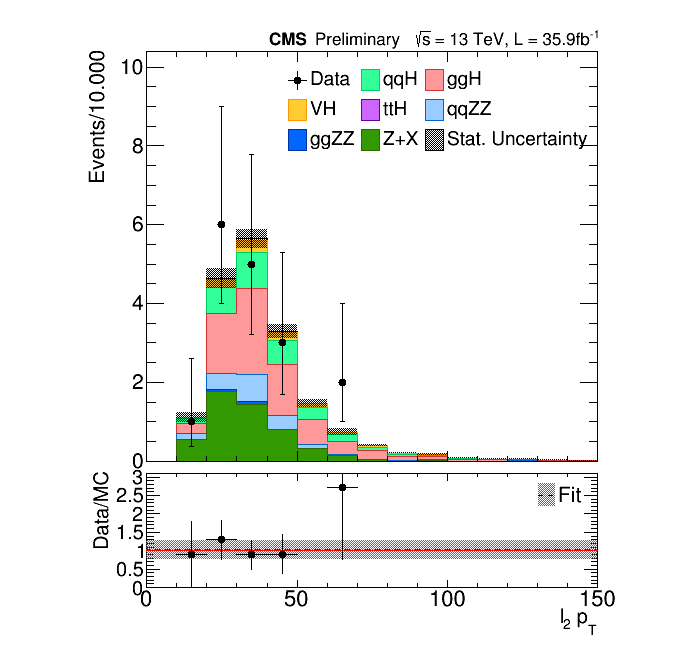
\includegraphics[scale=0.23,trim={2cm 1cm 2cm 1cm},clip]{ChapterAnalysis/figs/vbf_l2_pt}
	}
	\subfloat[]{
		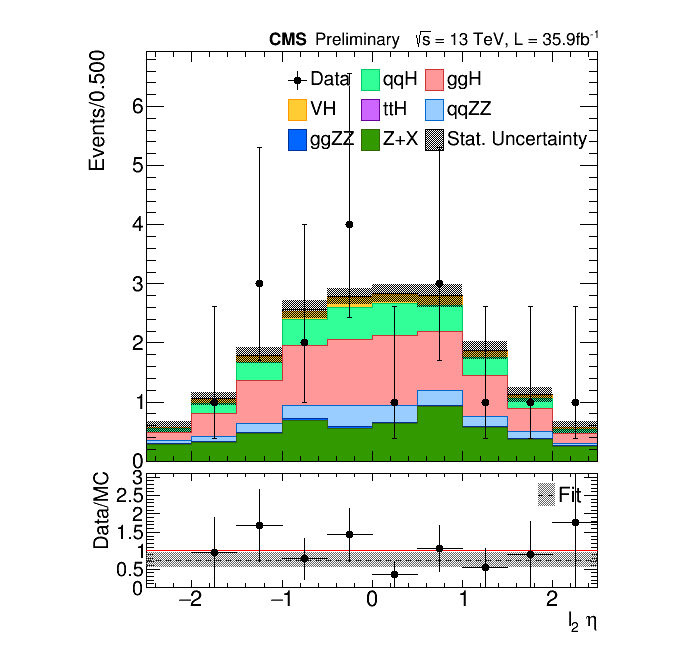
\includegraphics[scale=0.23,trim={2cm 1cm 2cm 1cm},clip]{ChapterAnalysis/figs/vbf_l2_eta}
	}
	\subfloat[]{
		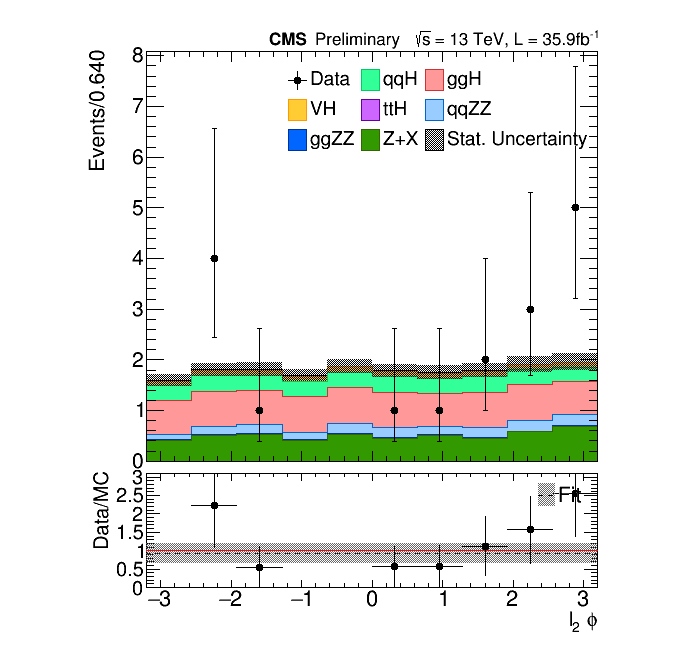
\includegraphics[scale=0.23,trim={2cm 1cm 2cm 1cm},clip]{ChapterAnalysis/figs/vbf_l2_phi}
	}\\
	\subfloat[]{
		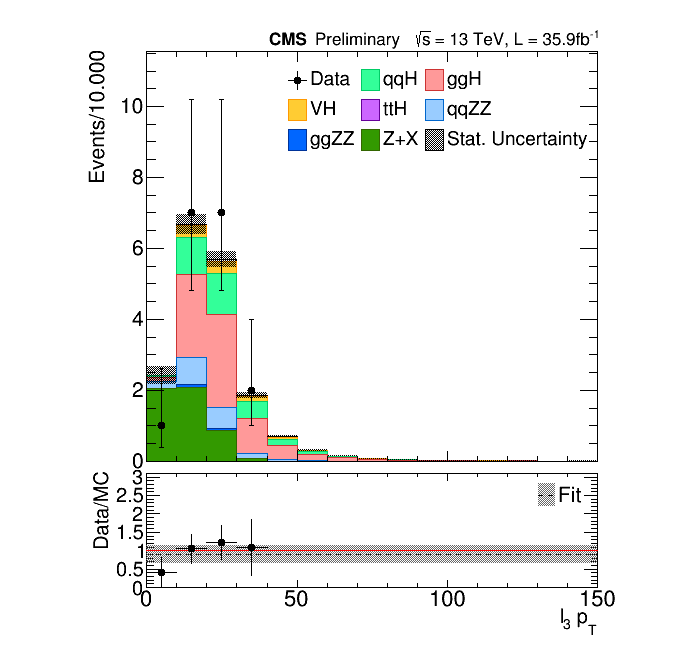
\includegraphics[scale=0.23,trim={2cm 1cm 2cm 1cm},clip]{ChapterAnalysis/figs/vbf_l3_pt}
	}
	\subfloat[]{
		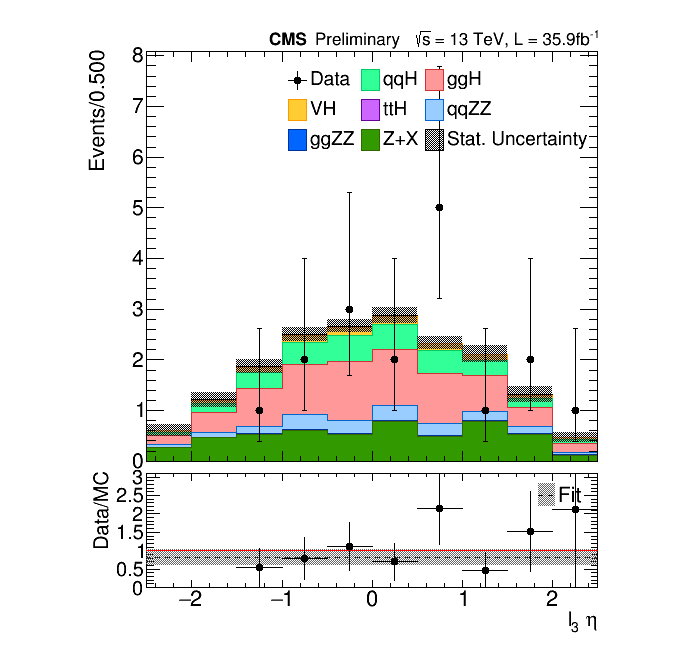
\includegraphics[scale=0.23,trim={2cm 1cm 2cm 1cm},clip]{ChapterAnalysis/figs/vbf_l3_eta}
	}
	\subfloat[]{
		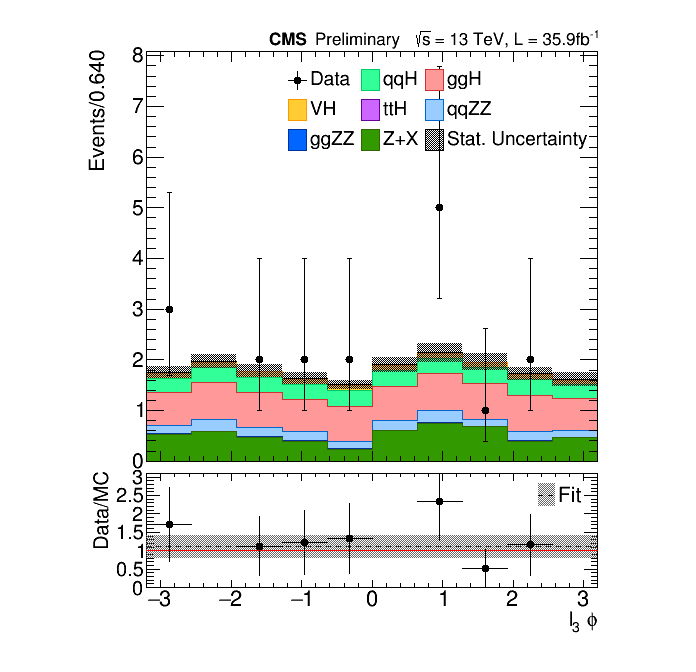
\includegraphics[scale=0.23,trim={2cm 1cm 2cm 1cm},clip]{ChapterAnalysis/figs/vbf_l3_phi}
	}\\
	\subfloat[]{
		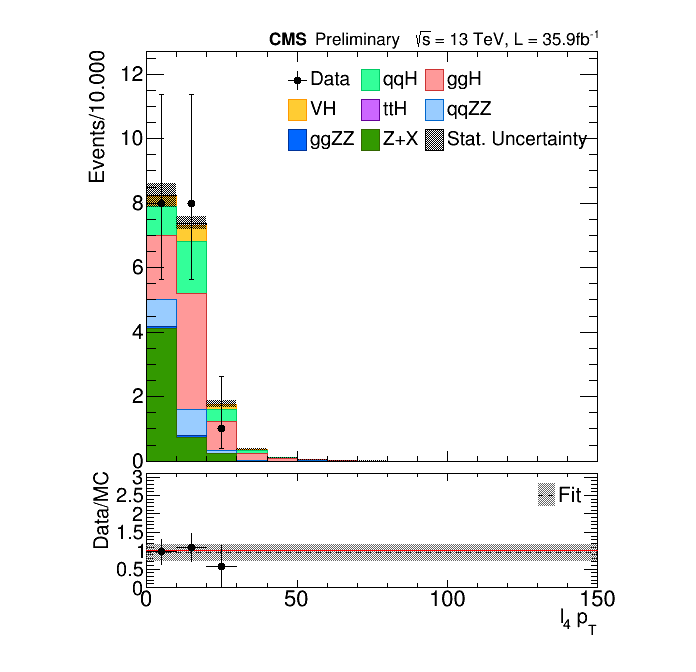
\includegraphics[scale=0.23,trim={2cm 1cm 2cm 1cm},clip]{ChapterAnalysis/figs/vbf_l4_pt}
	}
	\subfloat[]{
		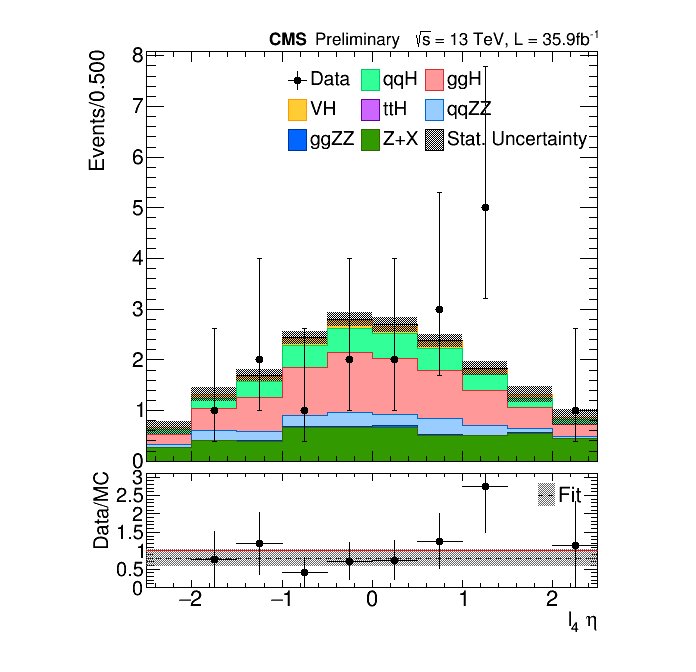
\includegraphics[scale=0.23,trim={2cm 1cm 2cm 1cm},clip]{ChapterAnalysis/figs/vbf_l4_eta}
	}
	\subfloat[]{
		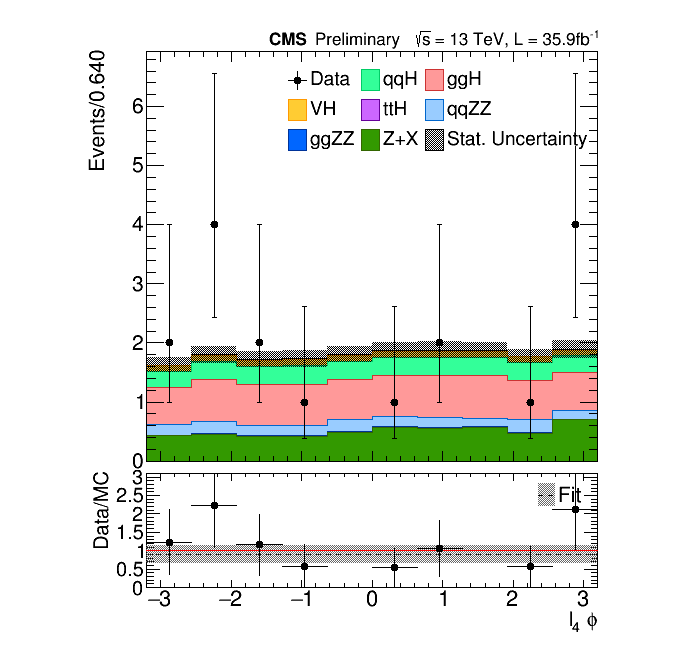
\includegraphics[scale=0.23,trim={2cm 1cm 2cm 1cm},clip]{ChapterAnalysis/figs/vbf_l4_phi}
	}
\end{figure}
\begin{figure}[hbtp]{16cm}
	\ContinuedFloat
	\centering
	\subfloat[]{
		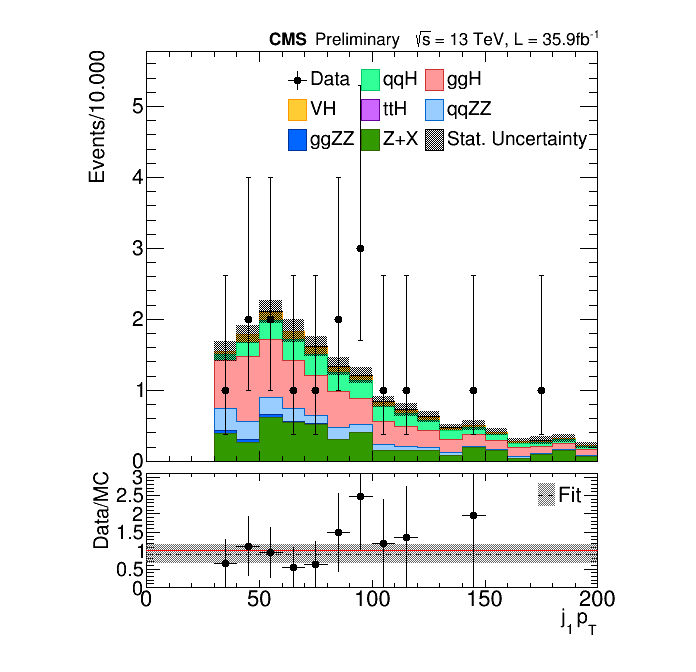
\includegraphics[scale=0.23,trim={2cm 1cm 2cm 1cm},clip]{ChapterAnalysis/figs/vbf_j1_pt}
	}
	\subfloat[]{
		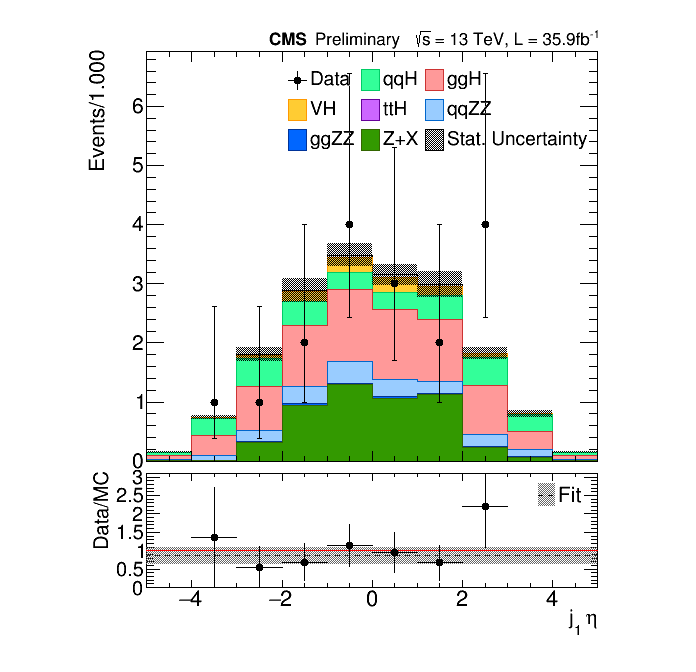
\includegraphics[scale=0.23,trim={2cm 1cm 2cm 1cm},clip]{ChapterAnalysis/figs/vbf_j1_eta}
	}
	\subfloat[]{
		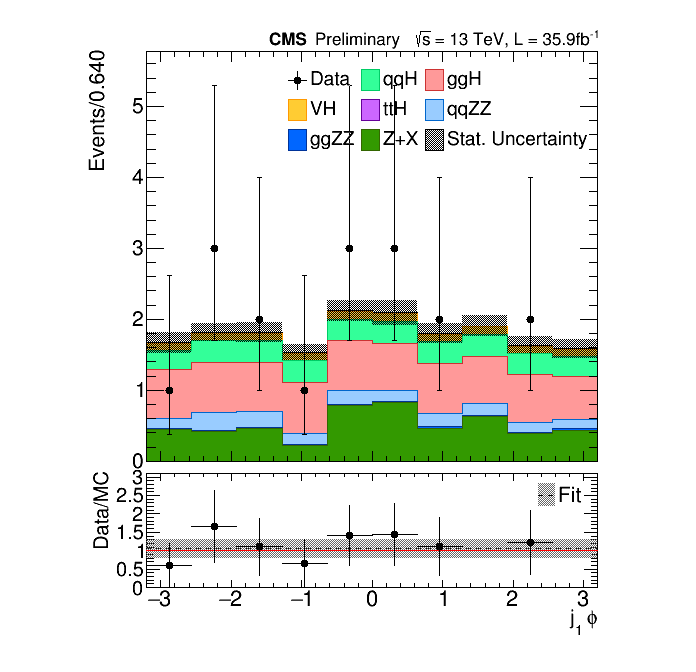
\includegraphics[scale=0.23,trim={2cm 1cm 2cm 1cm},clip]{ChapterAnalysis/figs/vbf_j1_phi}
	}\\
	\subfloat[]{
		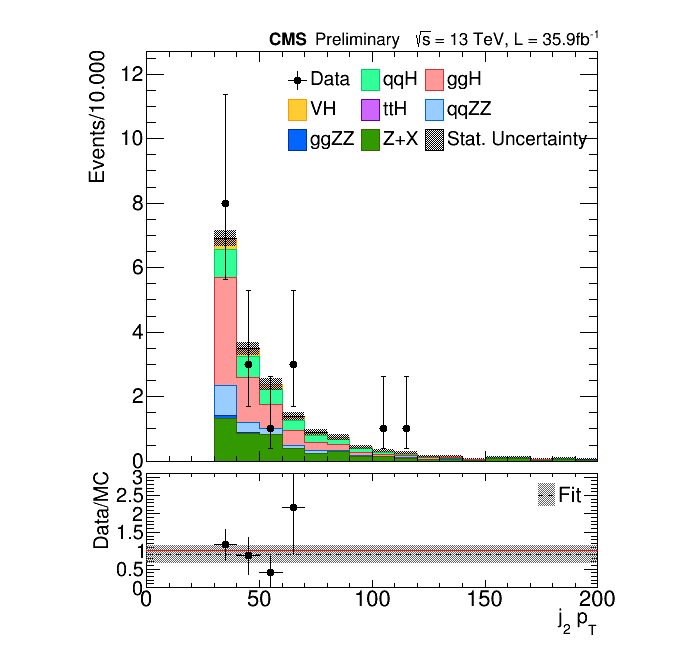
\includegraphics[scale=0.23,trim={2cm 1cm 2cm 1cm},clip]{ChapterAnalysis/figs/vbf_j2_pt}
	}
	\subfloat[]{
		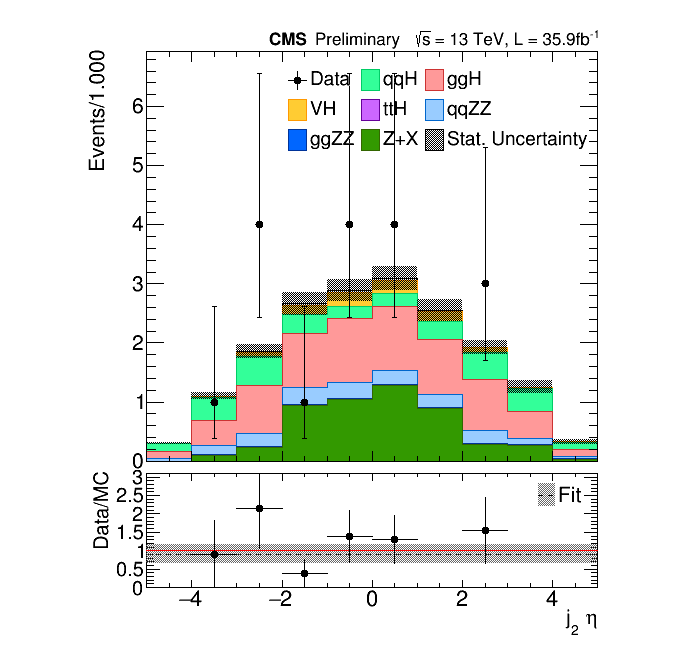
\includegraphics[scale=0.23,trim={2cm 1cm 2cm 1cm},clip]{ChapterAnalysis/figs/vbf_j2_eta}
	}
	\subfloat[]{
		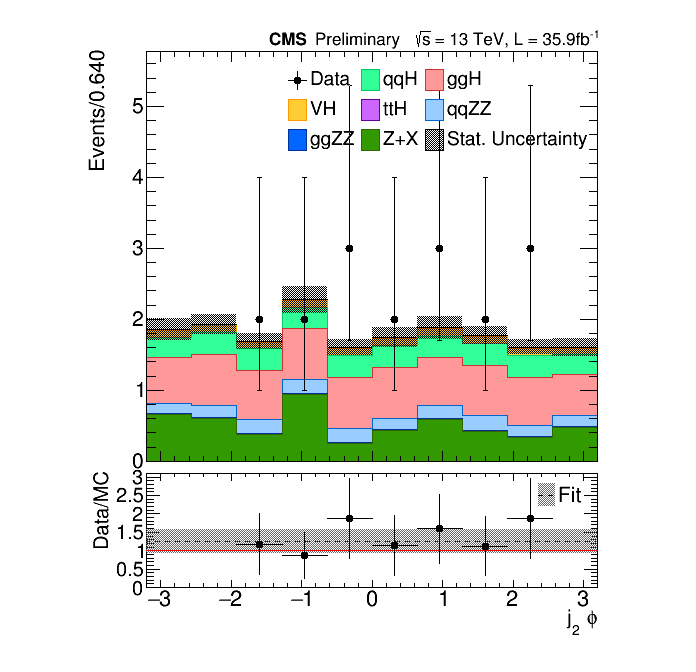
\includegraphics[scale=0.23,trim={2cm 1cm 2cm 1cm},clip]{ChapterAnalysis/figs/vbf_j2_phi}
	}\\
	\subfloat[]{
		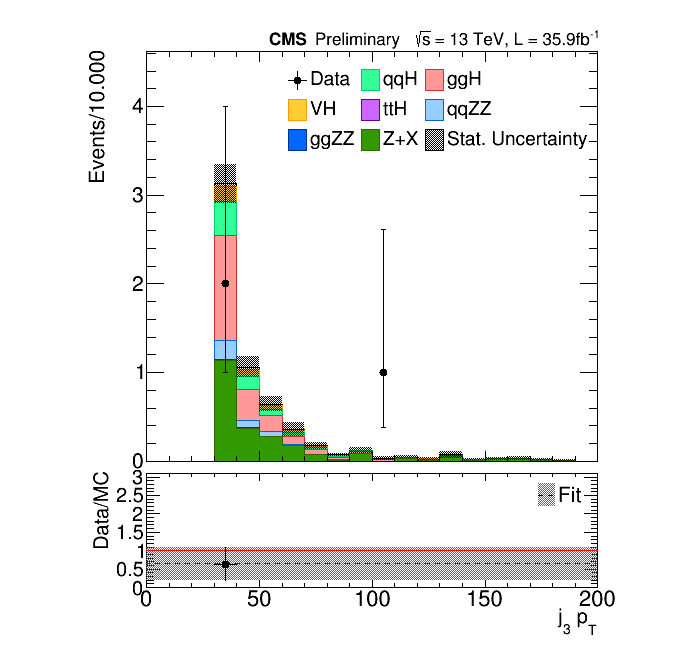
\includegraphics[scale=0.23,trim={2cm 1cm 2cm 1cm},clip]{ChapterAnalysis/figs/vbf_j3_pt}
	}
	\subfloat[]{
		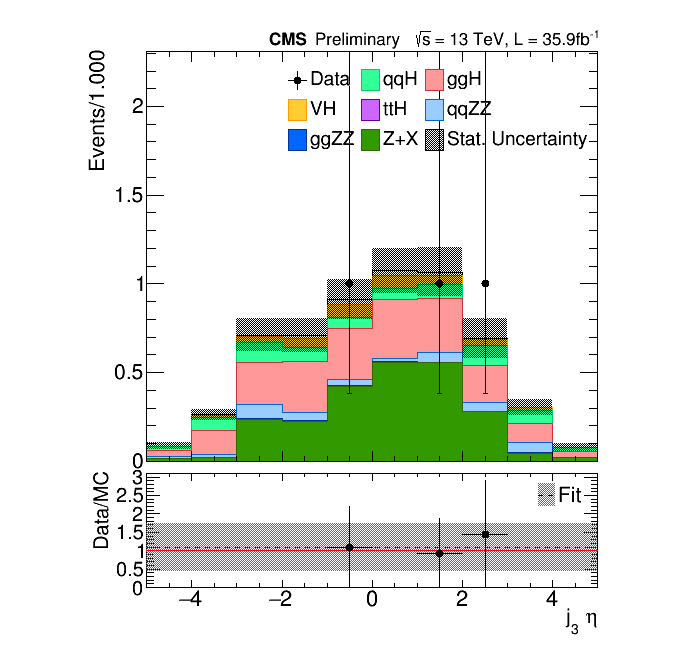
\includegraphics[scale=0.23,trim={2cm 1cm 2cm 1cm},clip]{ChapterAnalysis/figs/vbf_j3_eta}
	}
	\subfloat[]{
		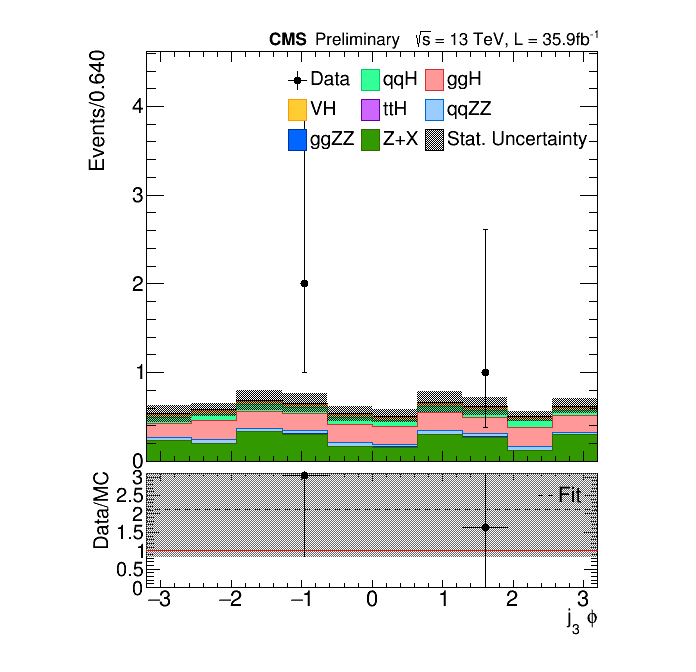
\includegraphics[scale=0.23,trim={2cm 1cm 2cm 1cm},clip]{ChapterAnalysis/figs/vbf_j3_phi}
	}	
	\source{The author, 2018.}
	\label{fig:ann_input_variables}
\end{figure}


In order to optimize the analysis and properly handle the usage of the third jet in the events, two jet-based categories have been defined and are labeled as \textbf{Njet2} and \textbf{Njet3} from now on. The \textbf{Njet2} category comprehend the events with exactly two jets while the \textbf{Njet3} category are composed by the events with at least three jets. For each of this category a ANN was developed.

Assuring an adequate distribution of the events when splitting them, forming the exclusive training and testing sets, the following procedure was adopted for the VBF-SR events in each jet-based category:
\begin{itemize}
	\item[1] Each simulated process has three samples one for each final state ($4\mu$, $4e$ and $2e2\mu$). Those three samples were merged into just a single sample with the events from each final state being randomized, such that the final states randomly populated the merged sample;
	\item[2] The merged and randomized samples for each process were divided into two parts: one containing $80\%$ of the total events and one containing the remaining $20\%$;
	\item[3] The first and second parts from each process were merged and once more the events were randomized in order to randomly populate each process inside the two parts;
\end{itemize}

The merged first parts constitutes the training set, that is the set of events used to train the ANN. The merged second parts constitute the testing set which is used to test the trained ANNs. Note that the two sets are completely independent such that the ANN was tested with completely new (and thus unseen by the ANN) events. As explained in Chapter~\ref{sec:neural_networks} the ANN training is very similar to a fit procedure and thus few examples (points) produces fits with large errors.

\section{Scaling Events Contribution in the Training}
\label{subsec:scale_train}
In the beginning of this analysis the ANN trainings were carried out without taking into account any kind of event weight. In such way all events are seen by the ANN in an equal basis. Keras has some features that allows one to include scale factor (a weight for each example event) which are in general used to balance the training when the number of events from different classes are very different. In the physics scenario one could use the individual MC event weights ($\sigma.\epsilon.BR$) or yet the sum of those weights (which constitutes the expected yields). The advantage of the first approach is that some events, from signal or background, crossing the classes zones defined by the ANN could have small weights and would be worthy to allow them to come in with the benefit to possibly improve  the final discrimination. The disadvantage is that the individual weights might not keep the hierarchical contribution of each process since the expected cross-section is divided by the number of events (such that if one have a large number of events the weights might become smaller for important processes than the ones for other small processes).

Both approaches were tested. The weight is used by Keras as a scale factor for the \textit{loss} function such that during the training each example is seen by the ANN with a different importance. That affects the direction in which the \textit{minimizer} computes the gradients of the \textit{loss} function. The advantage of doing so is that even if a process has few events, which is very frequent in many analysis, it will be properly taken into account with respect to the other process having more events. The Fig.~\ref{fig:scaling_training_effect} shows the impact of scaling the \textit{loss}. In the beginning of the analysis the sample ggH-minlo was produced slightly different from the other samples: the leptons were sorted by $p_{T}$ in the $4\mu$ final state. Without weighting the events during the training the typical ROC curves\footnote{ROC stands for Receive and Operative Curve which is a figure of merit commonly used in fields like medicine and shows a discriminant efficiency for filtering out signal versus background.} observed were like the one showed in Fig.~\ref{fig:nn_no_scale_roc}. Once the weights were introduced the discrimination of VBF and ggH processes increased significantly as showed in Fig.~\ref{fig:nn_scale_roc}. Although this is not a physical property and thus had to be fixed, this shown the big importance of scaling the events contribution. It shows that the ANN may not learn some features from a process if a scaling is not applied. As seen in Tab.~\ref{tab:vbf_sr_yields} ggH has the biggest yield and has a relatively good number of events but still without weighting it the small difference was not taken into account by the ANN. Since there all the further developed studies were done with the events weighted.

\begin{figure}[hbtp]{16cm}
	\caption{ROC curves comparing the performance of a trained ANN, the VBF MELA discriminant and $D_{jet}$: (a) the performance of ANN without scaling the \textit{loss} and (b) performance after scaling the \textit{loss}.}
	\centering
	\subfloat[]{
		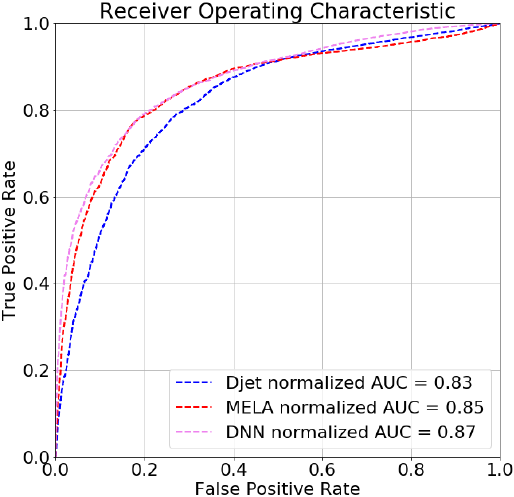
\includegraphics[width=0.35\textwidth]{ChapterAnalysis/figs/3jets_pt_eta_phi_no_weight_vbf_vs_all_leptons_sorting_issue}
		\label{fig:nn_no_scale_roc}
	}
	\quad
	\quad
	\subfloat[]{
		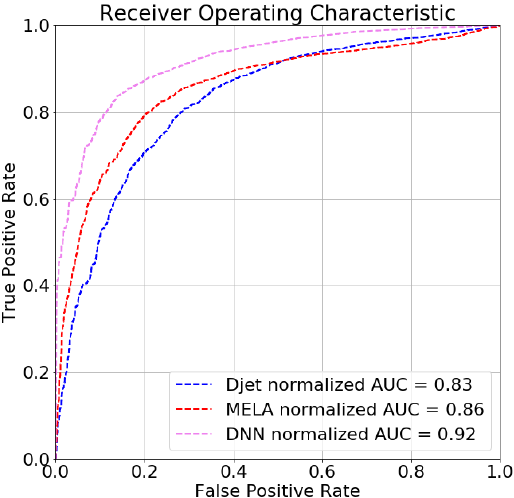
\includegraphics[width=0.35\textwidth]{ChapterAnalysis/figs/3jets_pt_eta_phi_weight_sum_vbf_vs_all_leptons_sorting_issue}
		\label{fig:nn_scale_roc}
	}
	\source{The author, 2018.}
	\label{fig:scaling_training_effect}
\end{figure}

\section{The Training Procedure}
\label{subsec:training_procedure}
Training MVA methods is a procedure that always need to be done in multiple fronts. It is hard to guarantee that for a set of inputs a set of MVA training parameters are the optimal choice, since there is an infinity of combinations that one can build. Those configurations (including the training dataset) can strongly affect the evolution of the MVA training. 

In the same time one needs to be careful when doing the training since crucial issues can occur and lead to a very bad MVA model. An ANN training commonly leads (or present them while on going) to one of three main situations: 
\begin{itemize}
\item \textbf{underfit}: occurs when an ANN has too few parameters (the $w_i$'s and $b_i$'s), making it not capable to model the training data. This behavior can be identified by looking the ANN loss curve not decreasing. Such issue can be, tentatively, solved by increasing the number of parameters (that is, using more neurons) and the training time. Notice though that the ANN will always reach some level where it can not learn more features from the training data, that is the ANN learning limit;
\item \textbf{goodfit}: this is the ideal situation. The ANN has a sufficient number of parameters and have been enough trained such that it properly models the training data and become able to make correct predictions on unseen data (that means the ANN is well generalized);
\item \textbf{overfit}: occurs when an ANN has too many parameters or is trained too much. In this situation the ANN starts to model the noise on the training data, that is, its variance (which is pretty common to happen in measured quantities). This usually makes the ANN very good in the modeling of the training data but it becomes very bad on making predictions for unseen data. This can be noticed by looking the training and the validation/testing loss diverging from each other and, usually the validation loss reaches a minimum and then starts to increase again. The best solution for this issue is the increasing of the training data set, which is not always possible. So, the other two tentative procedures are the reduction of the number of parameters and the reduction of the training time.
\end{itemize}

A good example of these three cases is show in Fig.~\ref{fig:training_issues}, which represents the situation of using an ANN to model a set of data distributed like sine/cosine shape. In Fig.~\ref{fig:training_issues}(a) the ANN had too few parameters and thus can't model the data distribution, while in (b) is has enough parameters such it can describe with good agreement the data. Fig.~\ref{fig:training_issues}(c) shows the extreme case when the ANN has too many parameters and thus has too many degrees of freedom to fit all data points. Since the loss is computed based on the difference between the ANN prediction and the original data, it goes very close to zero and one could think the ANN is perfect. However, as one let more data appear (which would be around the sine/cosine shape) it will see the ANN can't correctly predict such unseen data. Remember that on CMS collected data one does not know which physics process produced each event and thus is very important to have an ANN that can make right predictions on unseen Monte Carlo events.

\begin{figure}[hbtp]{16cm}
	\caption{Example of the three main situations that can occur during an ANN training: (a) the underfit, (b) the goodfit and (c) the overfit.}
	\centering
	\subfloat[]{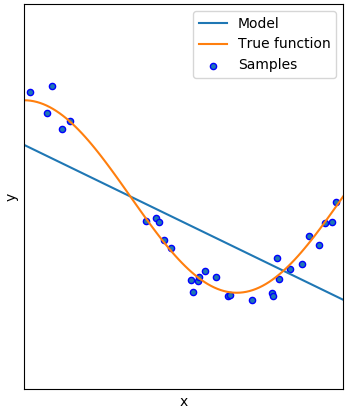
\includegraphics[scale=0.8]{Slides/figs/underfit}}
	\quad
	\subfloat[]{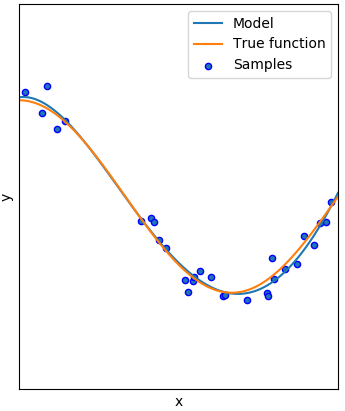
\includegraphics[scale=0.8]{Slides/figs/goodfit}}
	\quad
	\subfloat[]{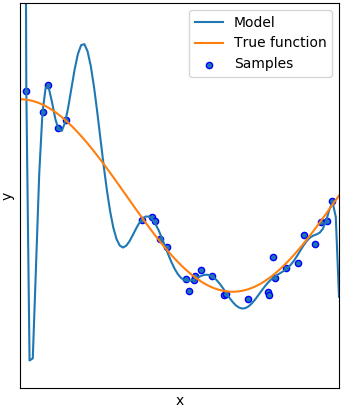
\includegraphics[scale=0.8]{Slides/figs/overfit}}
	\source{JORDAN, 2018.}
	\label{fig:training_issues}
\end{figure}

The underfit, goodfit and overfit can also be seen by looking the training and the validation/testing losses. This is a good thing when one can not compare the expectations to the ANN predictions as shown in Fig.~\ref{fig:training_issues}. A common recommendation found in the literature \cite{bib:SimonHaykin,bib:KevinGurney,bib:GlorotAndBendio2010,bib:NairAndHinton2010,bib:Zeiler_et_al2013,bib:glouppe-ESWB-2018-1} is represented in Fig.~\ref{fig:learning_curves} which shows the loss variation during an ANN training. The loss is the what is called "error" in the figure. As one can see the underfit and the overfit are two extremes situations in which the ANN are not good. It can either poorly model the data or poorly make reasonable predictions. The ideal point where to stop an ANN training is when the validation loss starts to increase and diverges from the training loss behavior.

\begin{figure}[hbtp]{16cm}
	\caption{The underfit, goofit and overfit seen from the training and validation/testing loss curves.}
	\centering
	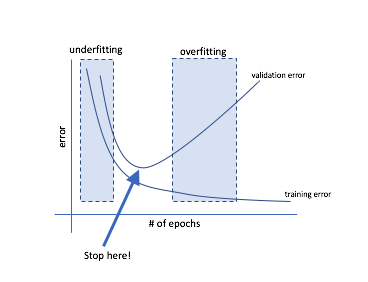
\includegraphics[scale=0.8,trim={2cm 0cm 0cm 2cm},clip]{Slides/figs/early_stop}
	\source{JORDAN, 2018.}
	\label{fig:learning_curves}
\end{figure}

In order to optimize the studies with the ANN in this analysis a framework was developed in python. It has the feature to build up through Keras different ANN architectures and perform multiple parallel scans. These scans can run over different sets of inputs and the several parameters that needs to be configured for the training. The result of each ANN training can be retrieved to produce plots which are used to validate and classify the quality of each training (one can check if over-fitting happened, for instance). 

The set of tested inputs includes combinations of the leptons and jets kinematic variables ($p_{T}$, $\eta$, $\phi$ and $E$), MET, Njets and Nbjets. The scanned ANN parameters are summarized in the Tab.~\ref{tab:training_parameters_summary}. These parameters are:
\begin{itemize}
	\item \textbf{Pre-processing}: it is a usual practice in Machine Learning field to apply some operation in the ANN inputs in order to standardize them (keep them in the same range of values for instance). In the scans done the pre-processing showed negligible effects and it was decided to not adopt such procedure for further studies. Note that, when pre-processing is applied in the training it will be need to also apply the same procedure when using the trained ANN (otherwise the results will be mistaken, since the ANN are expecting preprocessed inputs). One also should note that preprocessing changes the input variables what may destroy the possibility of the ANN reconstruct some important property(e.g. invariant masses);
	\item \textbf{Topology}: the architecture of the ANN, that is, the number of hidden layers, neurons and the neuron type. In Keras there are several types of neuron which even includes possible learning parameters (during training). The \textit{Rectified Linear Unity} (ReLU) is the most recommended due to its property of non-vanishing gradient;
	\item \textbf{Batch size}: the number of events in a subset from the training set used to compute the gradients and update the \textbf{$w_{i}$}'s and \textbf{$b$} in each neuron;
	\item \textbf{Epochs}: the number of iterations over the full training set. The total number of iterations is a combination of the size of the training set, the batch size and the number of epochs. For instance, setting a training of 10 epochs and a batch size of 10 for a training set size of 100 means that Keras performs $10^{2}$ updates on the \textbf{$w_{i}$}'s and \textbf{$b$}'s;
	\item \textbf{Early stop}: a parameter to set the number of epochs which Keras should wait if not improvement in the loss function is observed. If still not improvement is seen after that number of epochs the training is stopped;
	\item \textbf{Minimizer}: is the method to compute the gradients. There are several options in Keras (SGD, Adam, RMSprop, etc.) and after testing most of them it was decided to keep Adam. Adam stands for Adaptive Momentum and has the property of fast convergence due to a ANN updating directed towards the loss function minimum. This minimizer is widely applied in ML studies;
	\item \textbf{Scaling}: Keras allows one to scale the loss function by some weight that can be independent for each training example or the same for a entire class (signal or background, for instance). It was tested the impact of using the expected yield (cross section) of each process and the individual weights of each event ($\sigma.\epsilon.BR$);
	\item \textbf{Dropout}: it is a procedure in which keras randomly sets a fraction of the input units (literally the ANN input variables or then neurons outputs - which are inputs for forward neurons in the net) to zero at each update during the ANN training. This mechanism helps to prevent the over-fitting issue and also can build up more complex models. Keras allows one to apply this procedure in each layer independently (so one can apply it just on the first layer and not in the other ones);
\end{itemize}

\begin{table}[hbtp]{16cm}
	\centering
	\caption{Summary of the scanned parameters during ANN trainings.}
	\begin{tabular}{c|l}
		\hline
		\rowcolor{light_gray}
		Parameter      & Tested options\\
		\hline
		Inputs         & leptons/jets($p_{T}$,$\eta$,$\phi$), MET\\
		\hline
		Pre-processing & none, normalization, standardization\\
		\hline
		Topologies     & 7:5:3, 9:7:5, 11:9:7, 15:10:5, 21:13:8, 10:10:10:10, 30, 100, 100:100:50, 10$^{3}$\\
		\hline
		Early stop     & 100, 600, 3000\\
		\hline
		Minimizer      & SGD, Adam, Adagrad, Adadelta, RMSprop\\
		\hline
		Batch size     & 1, 5, 32, 64, 128, 786\\
		\hline
		Neuron         & ReLU, SeLU\\
		\hline
		Loss Scaling   & cross section, $\sigma.\epsilon.BR$ (event weight)\\
		\hline
		Dropout        & none, 0.1, 0.3, 0.5, 0.7, 0.9, 0.99, 0.3:0.4:0.2, 0.5:0.25:0.1\\
		\hline
	\end{tabular}
	\source{The author, 2018.}	
	\label{tab:training_parameters_summary}	
\end{table}

The ANNs achieved through these trainings are produced together with some plots which are used to validate the choice of the best ANN architecture. These plots comprehend the metrics adopted (ROCs, $\epsilon_{s}.\pi$, $\sigma$) and the ANN distributions for the training and test sets, which helps to check if there was over-fitting for a given configuration. Fig.~\ref{fig:nn_training_outputs} shows these plots. The ROCs curve from training and test sets are also used to check if there was over-fitting. The plots in Fig.~\ref{fig:nn_training_outputs} show a example in which the ANN is considered good.

\begin{figure}[hbtp]{16cm}
	\caption{Example of checking plots produced during ANNs training. (a) $D_{qqH, 2j}^{MELA}$ (for reference) and (b) ANN distributions, (c) $\epsilon_{s}.\pi$ vs $\epsilon$, (d) signal significance and (e) ROC curves computed using all backgrounds together for training and testing sets. (f) ROC areas computed separately for each background using the testing set (the filled lines are for the ANN and the dotted ones are for $D_{qqH, 2j}^{MELA}$).}
	\centering		
	\subfloat[]{
		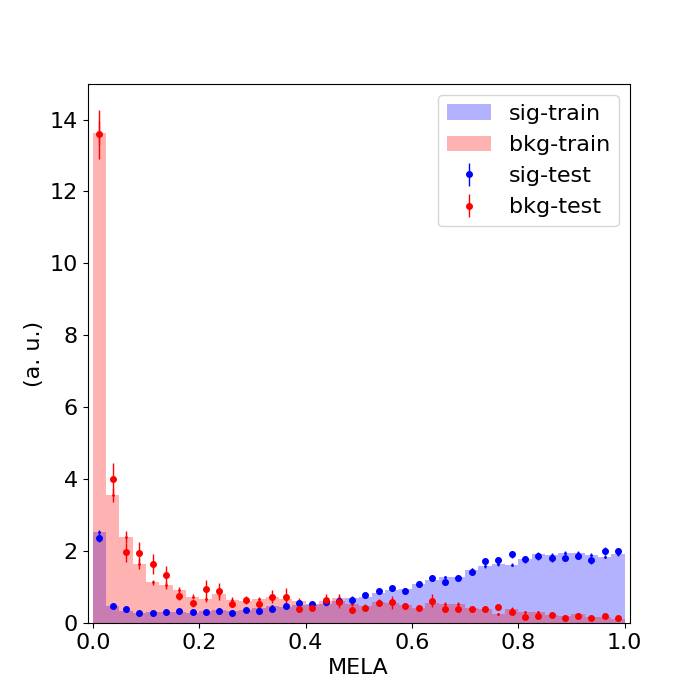
\includegraphics[scale=0.35]{ChapterAnalysis/figs/MELAOvertrainingCheck_example}
		\label{}
	}
	\subfloat[]{
		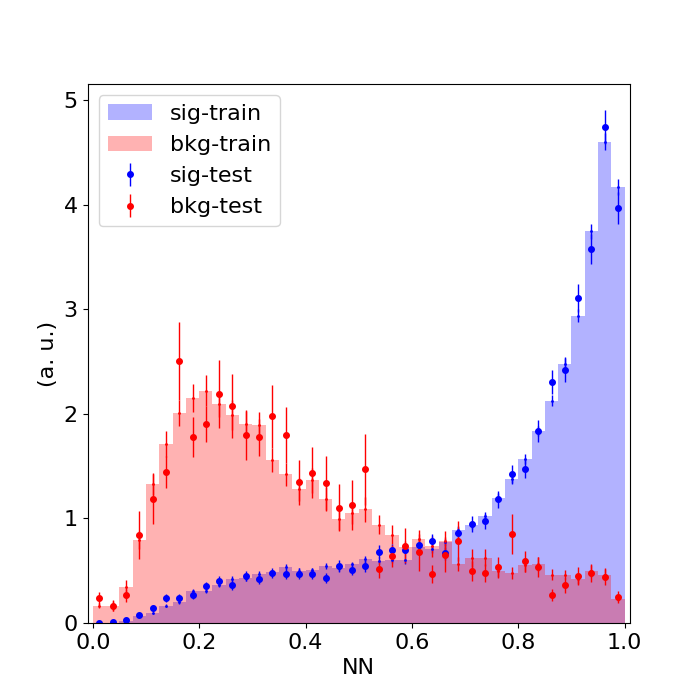
\includegraphics[scale=0.35]{ChapterAnalysis/figs/NNOvertrainingCheck_example}
		\label{}
	}\\		
	\subfloat[]{
		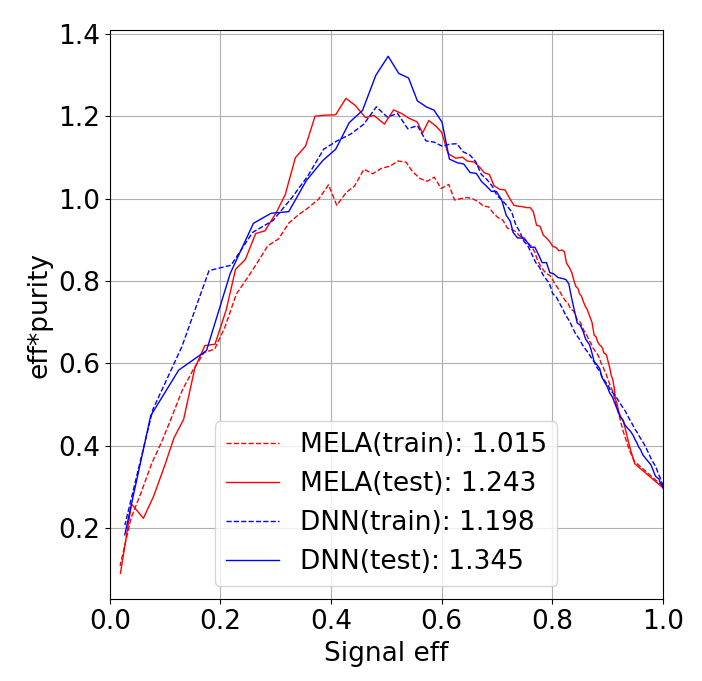
\includegraphics[scale=0.34]{ChapterAnalysis/figs/ComparisonMCsEffPurity_example}
		\label{}
	}
	\subfloat[]{
		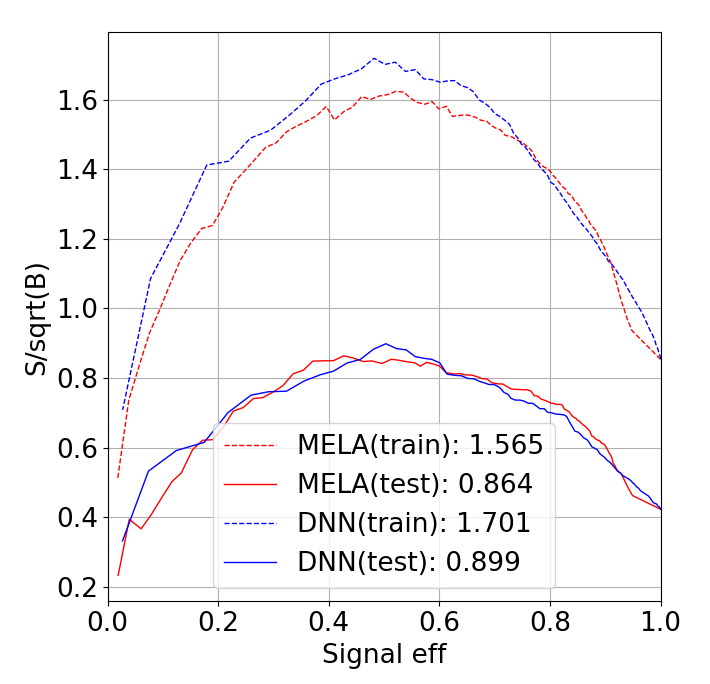
\includegraphics[scale=0.34]{ChapterAnalysis/figs/ComparisonMCsSignificance_example}
		\label{}
	}\\
	\subfloat[]{
		\includegraphics[scale=0.24]{ChapterAnalysis/figs/FinalTrainTestROCs_example}
		\label{}
	}
	\subfloat[]{
		\includegraphics[scale=0.24]{ChapterAnalysis/figs/ComparisonMCsROC_example}
		\label{fig:separated_rocs}
	}	
	
	\source{The author, 2018.}	
	\label{fig:nn_training_outputs}
\end{figure}


\section{NNs Training Performances}
In order to better visualize the results from the several scannings and choose the best ANN configuration, the metric $\epsilon_{s}.\pi$ were chosen to be the one representing the ANNs performance score. The Fig.~\ref{fig:nn_mela_scannings} shows a summary of those scannings. It is the difference in terms of $max(\epsilon_{s}.\pi)$ between each ANN and the $D_{qqH, 2j}^{MELA}$ applied to the same testing set.

From those several ANN trainings, some observations were drawn:
\begin{itemize}
	\item[1] As expected the jets are the objects which have almost all the discrimination power for VBF against the backgrounds. This is clear by noticing that when only the leptons are used the ANNs performance are very low (for any configuration). And also, noticing that with only the jets there were ANNs with performance similar to $D_{qqH,2j}^{MELA}$;
	\item[2] $p_{T}$, $\eta$ and $\phi$ seems to be enough for the discrimination. As can be noticed adding jet energy caused some trouble and none of the attempted configuration got better performance than when not using the jet energy;
	\item[3] Additional jets lead to more discrimination power. Different from $D_{qqH,2j}^{MELA}$, the ANNs can use information from extra jets (njets $>$ 2) when those are present in the event;
	\item[4] The usage of MET, Njets and Nbjets produced an increasing in performance similar to the ones observed when extra jets are used. For the final ANNs, Njets and Nbjets were not used since it is not straightforward how to estimate their systematic uncertainty.
\end{itemize}

\begin{figure}[hbtp]{16cm}
	\caption{Summary of the results obtained with the parameters scanning. The plot shows the difference between trained ANNs and $D_{qqH,2j}^{MELA}$ in three metrics used at that moment: max($\epsilon_{s}.\pi$), ROC area and significance}
	\centering
	\subfloat[]{\includegraphics[scale=0.35,trim={1.2cm 8.5cm 0.5cm 2.1cm},clip]{ChapterAnalysis/figs/SummaryOfResults_Metrics_Njets2_test_inputs}}
	\subfloat[]{\includegraphics[scale=0.35,trim={1.2cm 8.5cm 0.5cm 2.1cm},clip]{ChapterAnalysis/figs/SummaryOfResults_Metrics_Njets2_test_topology}}\\
	\subfloat[]{\includegraphics[scale=0.35,trim={1.2cm 8.5cm 0.5cm 2.1cm},clip]{ChapterAnalysis/figs/SummaryOfResults_Metrics_Njets2_test_minimizer}}
	\subfloat[]{\includegraphics[scale=0.35,trim={1.2cm 8.5cm 0.5cm 2.1cm},clip]{ChapterAnalysis/figs/SummaryOfResults_Metrics_Njets2_test_neuron}}\\
	\subfloat[]{\includegraphics[scale=0.35,trim={1.2cm 8.5cm 0.5cm 2.1cm},clip]{ChapterAnalysis/figs/SummaryOfResults_Metrics_Njets2_test_scaletrain}}
	\subfloat[]{\includegraphics[scale=0.35,trim={1.2cm 8.5cm 0.5cm 2.1cm},clip]{ChapterAnalysis/figs/SummaryOfResults_Metrics_Njets2_test_nooutliers}}
	\source{The author, 2018.}	
	\label{fig:nn_mela_scannings}	
\end{figure}

The final ANN for each of the jet-based categories were chosen to be the one with highest $max(\epsilon_{s}.\pi)$ and are presented in Chapter~\ref{subsec:statistical_analysis}. For the seek of the reader in Appendix~\ref{app:nns_architecture} the architecture of the two final ANNs can be seen. They give an idea of the correlation between the input variables. 

\subsection{The Impact of the VBF 3$^{rd}$ Jet}
The usual VBF process is characterized by the presence of two high energetic jets with a big gap between them on $\eta$, where the particle activity is rather small or even inexistent around it. This is the LO process. However, is possible that more jets appear in a VBF process and such jets are radiative corrections (higher order diagrams - NLO) which contributes for the total VBF cross section. These extra jets can contribute for discriminate the VBF process against the backgrounds.

Looking into the number of events which has extra jets one sees that there is a significant fraction for $VBF$, $ggH$, $qqZZ$ and even the observed data events with at least 3 jets. These fractions are in Tab.~\ref{tab:3rd_jet_events}. The usage of the ANNs including a 3$^{rd}$ jet in the events indicated at the beginning of this analysis that one could improve the discrimination between VBF and the background. Fig.~\ref{fig:comparison_2j_3j} shows that the ANNs present similar behavior as the MELA for a case with only two jets, while they show a improvement when the $3^{rd}$ jet is present as an input for the ANN. This is where the motivation to use the 3$^{rd}$ jet comes from in the present analysis.

\begin{table}[hbtp]{16cm}
	\centering
	\caption{Fraction of events, after the VBF-SR selections, containing the $jet_{i}$ (i-th jet).}
	\begin{tabular}{c|c|c}
		\hline
		\rowcolor{light_gray}
		       & $j_{3}(\%)$ & $j_{4}(\%)$\\
		\hline
		$qqH$  & 21.3        & 5.0\\
		\hline
		$ggH$  & 28.8        & 7.1\\
		\hline
		$qqZZ$ & 19.5        & 2.9\\
		\hline
		$Data$ & 18.0        & 0.0\\
		\hline
	\end{tabular}
	\source{The author, 2017.}
	\label{tab:3rd_jet_events}
\end{table}

\begin{figure}[htbp]{16cm}
	\caption{Performance of VBF discrimination against the backgrounds for the ANN, MELA and Djet discriminants. On (a) is the performance when considering only 2 jets per event and on (b) when considering up to 3 jets per event.}
	\centering
	\begin{overpic}
		[scale=0.5]{ChapterAnalysis/figs/2jets_dnn_mela_djet_rocs_hjj}
		\put(12,85){\color{red}2jets}
		\put(45,26){\includegraphics[height=3.5cm,width=3.5cm]{ChapterAnalysis/figs/2jets_sb_seff}}
		\put(50,-15){(a)}
	\end{overpic}
	\quad
	\begin{overpic}
		[scale=0.5]{ChapterAnalysis/figs/3jets_split0p8_norm_roc_djet_mela_dnn_hjj}
		\put(12,85){\color{red}3jets}
		\put(45,26){\includegraphics[height=3.5cm,width=3.5cm]{ChapterAnalysis/figs/3jets_sb_seff}}
		\put(50,-15){(b)}
	\end{overpic}	
	\source{The author, 2017.}
	\label{fig:comparison_2j_3j}
\end{figure}
	

%==========================================================================
\chapter{Background Estimation}
\label{sec:bkg_estimation}
%==========================================================================
In this analysis the backgrounds are composed by the three SM Higgs production modes, gluon fusion ($ggH$), associated vector ($WH$, $ZH$) and $t\bar{t}H$, and the SM backgrounds $q\bar{q} \rightarrow ZZ$, $gg \rightarrow ZZ$ and $Z+X$.

%==========================================================================
\section{Estimation of the SM Higgs Production Modes}
\label{sec:smhiggs_other_modes}
%==========================================================================
The SM Higgs production modes are estimated from MC by normalizing the yields according to the cross sections times the branching ratio fractions ($\sigma~.~BR$) as computed by the LHC Higgs Cross Section Working Group \cite{bib:CMS-AN-16-328}.

%==========================================================================
\section{Modeling of $q\bar{q} \rightarrow ZZ$}
\label{sec:qqzz_modeling}
%==========================================================================
The $q\bar{q} \rightarrow ZZ$ background events are generated at NLO. The fully differential cross section, which is not yet available in a partonic level event generator, is computed at NNLO. NNLO/NLO \textit{k}-factors are then applied to the $q\bar{q} \rightarrow ZZ$ NLO POWHEG sample. The inclusive cross sections obtained using the same PDF, as well the renormalization and factorization scales, as the POWHEG LO, NLO and NNLO are used. The NNLO/NLO \textit{k}-factors are applied as function of $m_{ZZ}$ \cite{bib:CMS-AN-16-328, bib:CMS-AN-16-442}.

Additional NLO electroweak corrections, which depend on the initial state quark flavor and kinematics, are also applied in the mass range of $m_{ZZ} >$ $2m_{Z}$, where the corrections have been computed \cite{bib:CMS-AN-16-442}.

%==========================================================================
\section{Modeling of $gg \rightarrow ZZ$}
\label{sec:ggzz_modeling}
%==========================================================================
The $gg \rightarrow ZZ$ background is generated at LO with the generator MCFM 7.0 \cite{bib:NPPS-10-205}. This background does not have exact calculation beyond LO. However, it has been shown that the soft collinear approximation is able to describe such background cross section and the interference term at NNLO \cite{bib:PhysRevD-88-2013-034032}. Also, the k-factors are very similar at NLO for signal (Higgs) and background \cite{bib:PhysLettB-774-2015-43} and, at NNLO for signal and the interference terms \cite{bib:JHEP-1508-2015-065}. Because of that, the same k-factor is used for signal and background. The k-factor at NNLO for the signal is obtained as a function of $m_{4l}$ using the HNNLO v2 MC program by calculating the NNLO and LO $gg \rightarrow H \rightarrow 2l2l$ cross sections at the small H boson decay width of 4.07 MeV and taking their ratios \cite{bib:PhysRevLett-98-2007-222002, bib:JHEP-02-2008-043, bib:JHEP-09-2013-129}. The NNLO, as well the NLO, k-factors and the cross sections are reported in \cite{bib:CMS-AN-16-442} along with the NNLO, NLO and LO cross sections at the SM Higgs boson decay width.

%==========================================================================
\section{Estimation of Z+X Background}
\label{sec:zx_estimation}
%==========================================================================
The commonly called Z+X background is a reducible background in the $H \rightarrow ZZ \rightarrow 4l$ analysis and originates from processes which contain one or more non-prompt leptons in the four-lepton final state. Non-prompt leptons are mainly non-isolated leptons which can originate from the heavy-flavor mesons decay, mis-reconstructed jets (usually coming from light-flavor quarks) and electrons from $\gamma$ conversions. Such non-prompt leptons are usually called "fake" leptons.

The estimation of such background in the $H \rightarrow ZZ \rightarrow 4l$ analysis is done by measuring the $f_{e}$ ($f_{\mu}$) probability of fake electrons (fake muons) passing the loose selection criteria (described in Chapter~\ref{sec:event_selection}) to also pass the final selection criteria (the \textit{tight} selection described in Chapter~\ref{sec:event_selection}). These probabilities are called as fake ratios or fake rates and are applied into two defined control regions (CRs) in order to extract the expected Z+X yield in the signal region.

In the following sections the steps needed for the estimation of Z+X yields and shape in this analysis are described.

\subsection{Measuring the Fake Rates}
\label{subsec:fr_method}
The measurement of the lepton fake rates requires a selection of samples of $Z_{ll}+e$ and $Z_{ll}+\mu$ events. Such events are expected to be dominated by a Z boson and a fake lepton. The leptons forming the $Z$ must be opposite sign, same flavor and have $p_{T} >$ 20(10) GeV. The third lepton ($e/\mu$) has to pass the loose selection and is used as the probe to compute the $f_{e}$ and $f_{\mu}$ probabilities. The invariant mass given by the fake lepton and the opposite-sign tight lepton composing the Z is required to be $m_{ll} >$ 4GeV to reduce QCD contamination. Also, in order to suppress contamination from $\gamma$ conversions to electrons the invariant mass of the two leptons composing the $Z$ must satisfy $|m_{Z_{ll}}-m_{Z}| <$ 7GeV. The remaining events are expected to also contain contribution from $WZ$ and $t\bar{t}$, which are reduced by requiring $E_{T}^{miss} <$ 25GeV.

The fake rate is parameterized in terms of the probe lepton $p_{T}$ and $\eta$. It has been shown in \cite{bib:CMS-AN-16-328} that there is no dependence between the fake rate and the probe lepton charge. Fig.~\ref{fig:fake_rates} shows the fake rate estimation separately for electrons and muons in terms of $p_{T}$ and $\eta$.

There are two FR distributions in Fig.~\ref{fig:fake_rates}. The points with solid error bars are the fake rates computed directly from data through the procedure described above. But, since $WZ$ background potentially contributes with three real leptons and such background is already included in the analysis via MC, it is then subtracted from data (separately in the numerator and in the numerator used to compute the FR's). The resulting FR after this subtraction is shown by the points with dotted error bars in Fig.~\ref{fig:fake_rates}. 

\begin{figure}[htbp]{16cm}
	\caption{Fake rates in terms of the lepton probe $p_{T}$ and $\eta$. The $p_{T}$ distributions (barrel and endcap) corresponds to the regions defined by $|\eta| <$ 1.479 (1.2) for electrons (muons). The background $WZ$ from MC has been subtracted.}
	\centering
	\includegraphics[scale=0.5]{ChapterAnalysis/figs/fake_rate_1D_pt_eta}
	\source{The author, 2018.}	
	\label{fig:fake_rates}
\end{figure}

Now, as one can see, there is a significant dependence between the FR's and the ($p_{T}$, $\eta$) of the loose leptons. For this reason the final parameterization of the FR's is made as a function of these two variables and it is shown in the Fig.~\ref{fig:fake_rates_2d}. The binning used for such distributions have been chosen in order to control the statistical uncertainty across the bins and avoid large uncertainties on the FR's. The muon case is worse than electron due to low statistics in data.

\begin{figure}[htbp]{16cm}
	\caption{Fake rates as a function of the probe lepton $p_{T}$ and $\eta$. The background $WZ$ from MC has been subtracted. This is the mapping for fake rates applied into the control regions.}
	\centering
	\includegraphics[scale=0.37]{ChapterAnalysis/figs/fake_rate_2D_maps_corrected}
	\source{The author, 2018.}	
	\label{fig:fake_rates_2d}
\end{figure}

\subsection{Building Control Regions}
\label{subsec:os_method}
In order to apply the fake rates described previously, two control regions are defined requiring events with two leptons passing the selection of the first Z (tight leptons) and additionally a pair of loose leptons of same flavor, opposite charge and passing the $SIP_{3D}$ cut. These events also must satisfy all the kinematic cuts applied for the Higgs phase space selection (See section \ref{sec:event_selection}). 

The first control region is then built by requiring that the two loose leptons do not pass the final identification and isolation criteria. This control sample is nominated as "2Prompt + 2Fail" (being referred as 2P2F from now on) and it is expected to be populated by events that have only two prompt leptons: mostly $DY$ (Drell Yan) with a small fraction of $t\bar{t}$ and $Z\gamma$. 

The second control region is obtained by requiring that just one of the four leptons does not pass the final identification and isolation criteria. The remaining three leptons in the event should pass those selections. This control region is then nominated "3Prompt + 1Fail" (being referred as 3P1F from now on). The events appearing in this control region are the same present in the 2P2F, with different relative proportions though, plus WZ events that are expected to have three prompt leptons.

These two control regions, which are enriched by fake leptons, are orthogonal to the Higgs signal region and are used to estimate the yields and shape of the Z+X background in the signal region. The four lepton invariant mass for the 2P2F and 3P1F control regions, as obtained for data and simulation separated by final state, can be seen in the Fig.~\ref{fig:m4l_2p2f} and Fig.~\ref{fig:m4l_3p1f}.

The expected number of reducible background events in the 3P1F control region can be computed by weighting each event observed in the 2P2F control region with the factor ($\frac{f_{i}}{1-f_{i}}+\frac{f_{j}}{1-f_{j}}$), in which the $f$'s correspond to fake rates as derived from the map shown in Fig.~\ref{fig:fake_rates_2d} using ($p_{T}$, $\eta$) of each loose lepton. This estimation of 3P1F events from the 2P1F control region is shown in Fig.~\ref{fig:m4l_3p1f}. 

\begin{figure}[htbp]{16cm}
	\caption{Four-lepton invariant mass distribution of the events selected in the 2P2F control region in the 13TeV dataset: (a) 4$\mu$, (b) 4e, (c) 2$\mu$2e and (d) 2e2$\mu$ channels.}
	\centering
	\subfloat[]{\includegraphics[scale=0.3]{ChapterAnalysis/figs/m4l_2p2f_4mu_smhiggs}}
	\subfloat[]{\includegraphics[scale=0.3]{ChapterAnalysis/figs/m4l_2p2f_4e_smhiggs}}\\
	\subfloat[]{\includegraphics[scale=0.3]{ChapterAnalysis/figs/m4l_2p2f_2mu2e_smhiggs}}
	\subfloat[]{\includegraphics[scale=0.3]{ChapterAnalysis/figs/m4l_2p2f_2e2mu_smhiggs}}
	\source{The author, 2018.}	
	\label{fig:m4l_2p2f}
\end{figure}

\begin{figure}[htbp]{16cm}
	\caption{Four-lepton invariant mass distribution of the events selected in the 3P1F control region in the 13TeV dataset: (a) 4$\mu$, (b) 4e, (c) 2$\mu$2e and (d) 2e2$\mu$ channels.}
	\centering
	\subfloat[]{\includegraphics[scale=0.3]{ChapterAnalysis/figs/m4l_3p1f_4mu_smhiggs}}
	\subfloat[]{\includegraphics[scale=0.3]{ChapterAnalysis/figs/m4l_3p1f_4e_smhiggs}}\\
	\subfloat[]{\includegraphics[scale=0.3]{ChapterAnalysis/figs/m4l_3p1f_2mu2e_smhiggs}}
	\subfloat[]{\includegraphics[scale=0.3]{ChapterAnalysis/figs/m4l_3p1f_2e2mu_smhiggs}}
	\source{The author, 2018.}
	\label{fig:m4l_3p1f}
\end{figure}

The discrepancy observed in the 2P2F control region for $Z_{1}+\mu\mu$ is related specially to the limited statistics of $Z+b\bar{b}$ and $Z+c\bar{c}$ events in the inclusive Z+jets sample (Drell Yan) as has been pointed previously in \cite{bib:CMS-AN-12-367,bib:CMS-AN-13-108}. The $Z_{1}+ee$ channels are better described by the available MC simulation. The discrepancies also arise because the fake rates do not properly take into account the background composition of 2P2F as detailed in Chapter~7.2 of \cite{bib:CMS-AN-16-442}.

In order to correct those discrepancies and correctly estimate the Z+X background, one needs two components:

\begin{itemize}
	\item a component directly from 2P2F, computed by weighting each observed event in the 2P2F control region using the factor ($\frac{f_{i}}{1-f_{i}}~\frac{f_{j}}{1-f_{j}}$), in which the $f$'s are the fake rates of loose leptons as explained before;
	\item a component from 3P1F, obtained by the difference between the observed events in 3P1F ($N_{3P1F}$), the expected contribution from 2P2F and from ZZ in the signal region ($N^{ZZ}_{3P1F}+N^{bkg}_{3P1F}$). The ZZ contribution is taken from the MC simulated events selected in the 3P1F control region. The $N^{bkg}_{3P1F}$ is the 3P1F extrapolation from 2P2F as discussed above.
\end{itemize}

the final expression for the estimation of Z+X can be then symbolically represented as,

\begin{equation}
N^{bkg}_{SR} = \sum \frac{f^{i}_{a}}{(1-f^{i}_{a})}(N_{3P1F}-N^{bkg}_{3P1F}-N^{ZZ}_{3P1F}) + \sum \frac{f^{i}_{b}}{(1-f^{i}_{b})} \frac{f^{j}_{c}}{(1-f^{j}_{c})} N_{2P2F}
\label{eq:zx_formula1}
\end{equation}

which is more conveniently expressed as,

\begin{equation}
N^{bkg}_{SR} = (1 - \frac{N^{ZZ}_{3P1F}}{N_{3P1F}}) \sum^{N_{3P1F}}_{i} \frac{f^{i}_{a}}{(1-f^{i}_{a})} - \sum^{N_{2P2F}}_{j} \frac{f^{j}_{b}}{(1-f^{j}_{b})} \frac{f^{j}_{c}}{(1-f^{j}_{c})}.
\label{eq:zx_formula2}
\end{equation}

The Eq.~\ref{eq:zx_formula2} represents what has been done to estimate the Z+X background contribution in this analysis. In order to get the appropriate yields and their statistical uncertainties the Eq.~\ref{eq:zx_formula2} is computed using histograms. The two sums are represented by two separated histograms with weights given by the fake rate fractions from the loose leptons. Then, the histogram representing the first sum (left one) is scaled by the multiplying term seen in Eq.~\ref{eq:zx_formula2}. In that term, $N^{ZZ}_{3P1F}$ and $N_{3P1F}$ are, respectively, the number of expected ZZ events (from MC) and the number of observed events selected in the 3P1F control region. Finally, the histogram representing the second sum (right one) is subtracted from the scaled histogram. This procedure is convenient to get not only the yields (which corresponds to the integral of the resulting histogram) and the statistical uncertainties correctly but, also the shape of Z+X. The yields computed in this way are shown in Tab.~\ref{tab:zx_os_yields} and the derived $m_{4l}$ shapes are shown in Fig.~\ref{fig:m4l_zx_os_shapes} for events after (a) SM Higgs and (b) VBF-SR selections.

\begin{table}[hbtp]{16cm}
	\centering
	\caption{Yields estimated for Z+X in the signal region from the measurements on data using the fake rate method with opposite-sign (OS) leptons. Estimates reported with statistical uncertainties comparing Higgs signal SR and after applying the cuts defining the VBF-SR.}
	\begin{tabular}{c|c|c|c|c}
		\hline
		\rowcolor{light_gray}
		Selection & 4$\mu$         & 4e             & 2e2$\mu$       & 4l\\
		\hline
		SM Higgs  & 24.28$\pm$0.60 & 27.80$\pm$1.81 & 56.90$\pm$2.11 & 108.99$\pm$2.84\\
		VBF-SR    &  2.03$\pm$0.18 &  0.33$\pm$0.20 &  2.72$\pm$0.17 &   5.08$\pm$0.32\\
		\hline
	\end{tabular}
	\source{The author, 2018.}
	\label{tab:zx_os_yields}
\end{table}

\begin{figure}[htbp]{16cm}
	\caption{Four-lepton mass distribution of Z+X for events after the (a) SM Higgs and (b) VBF-SR selections. The shapes are shown for each separate channel and for their combination into $4l$ final state.}
	\centering
	\subfloat[]{\includegraphics[scale=0.26]{ChapterAnalysis/figs/m4l_zx_4l_smhiggs}}
	\subfloat[]{\includegraphics[scale=0.26]{ChapterAnalysis/figs/m4l_zx_4l_vbf}}
	\source{The author, 2018.}
	\label{fig:m4l_zx_os_shapes}
\end{figure}


\subsection{Uncertainties on the Estimation of Z+X}
The statistical uncertainty on the Z+X estimation comes from the limited number of events selected in the control regions where one measures and applies the fake ratio methods. Such uncertainty is typically in the range of 2-7$\%$ (SM Higgs) and 8-61$\%$ (VBF-SR). The systematic uncertainty arises because the composition of reducible backgrounds in the control regions where one measures and applies the fake ratios are usually not the same. This is the main source of systematic uncertainty of the fake ratio method. This uncertainty is estimated in three steps. First, one measures the fake rates for each background process ($DY$, $t\bar{t}$, WZ, ZZ, Z$\gamma$) using MC and applying the selections explained in the Chapter~\ref{subsec:fr_method} to obtain samples of $Z+l$. Then, one defines the fake rates for MC (simulation) by computing the weighted average of those individual fake rates. Second, one reweights the individual fake rates using the expected yields of the reducible backgrounds selected in the 2P2F control region. Then, one applies the average and the re-weighted fake rates in order to get the final yields of Z+X and finally, the difference between them is used as an estimation of the uncertainty on the measurement of fake rates. The average and the re-weighted fake rates are shown in Tab.~\ref{tab:fake_rate_overall_systematic}.

\begin{table}[hbtp]{16cm}
	\centering
	\caption{The fake ratios for individual background processes, the average fake ratio and the fake ratio reweighed according to the composition of backgrounds in 2P2F control region.}
	\scriptsize
	\begin{tabular}{c|c|c|c|c|c|c|c}
		\hline
		\rowcolor{light_gray}
		FR    & $ZZ,~Z\gamma*$  & $WZ$            & $t\bar{t}+jets$ & $Z+jets$        & Average & Reweighed & Uncertainty ($\%$)\\
		\hline
		$e$   & 0.750$\pm$0.005 & 0.848$\pm$0.014 & 0.077$\pm$0.008 & 0.039$\pm$0.001 & 0.040$\pm$0.001 & 0.051$\pm$0.001  & 27.5\\
		$\mu$ & 0.899$\pm$0.007 & 0.963$\pm$0.017 & 0.165$\pm$0.020 & 0.114$\pm$0.002 & 0.118$\pm$0.002 & 0.134$\pm$0.003  & 13.3\\
		\hline
	\end{tabular}
	\source{The author, 2018.}	
	\label{tab:fake_rate_overall_systematic}	
\end{table}


The fake rates versus $p_{T}$ and $\eta$ computed for each reducible background are shown in Fig.~\ref{fig:fr_pt_eta_1D_systematics} and the 2D maps used to apply the fake rates can be seen in Fig.~\ref{fig:fr_pt_eta_1D_systematics}. The final yields for Z+X along with the statistical, systematic and combined uncertainties are shown in Tab.~\ref{tab:final_zx_estimation}.

\begin{landscape}
\begin{figure}[htbp]{23cm}
	\caption{Fake rate, for each reducible background ($DY$, $t\bar{t}$, WZ, ZZ, Z$\gamma$), the average and the re-weighted distributions for electron (a) $p_{T}$ barrel, (b) $p_{T}$ endcap and (c) $\eta$ and for muons (d) $p_{T}$ barrel, (e) $p_{T}$ endcap and (f) $\eta$.}
	\centering
	\includegraphics[scale=0.5]{ChapterAnalysis/figs/fake_rate_1D_pt_eta_for_systematics}
	\source{The author, 2018.}
	\label{fig:fr_pt_eta_1D_systematics}
\end{figure}
\end{landscape}

\begin{figure}[htbp]{16cm}
	\caption{Fake rate versus $p_{T}$ and $\eta$ for the average and the re-weighted distributions for electron (a) and (c) and, for muon (b) and (d), respectively.}
	\centering
	\includegraphics[scale=0.5]{ChapterAnalysis/figs/fake_rate_2D_maps_for_systematics}
	\source{The author, 2018.}	
	\label{fig:fr_pt_eta_2D_systematics}
\end{figure}


\subsection{Same-Sign Cross-checking and Final Z+X Estimation}
A cross-checking procedure (see \cite{bib:CMS-HIG-13-002,bib:CMS-AN-16-328}) is applied in order to verify the Z+X estimation from OS method by applying the selections used in the Same-Sign (SS) method. The SS method requires similar selections to get the 2P2F and 3P1F control regions explained in Chapter~\ref{subsec:os_method}. The events are obtained as a subset of the events satisfying the first step of the selection, which correspond to the first Z selection composed by two opposite-sign and same-flavor (SF) leptons. Additionally, one requires a pair of loose leptons same-sign (avoiding signal contamination) and same-flavor. The SS-SF leptons are requested to pass the $SIP_{3D}$ requirement (as previously in the OS method) and, now, also to pass both the identification and isolation criteria, which are imposed to the signal events. As for the SM Higgs selections one requires that $m_{ll} > 4$GeV (the QCD suppression cut between any two leptons), $12 < m_{ll} < 120$GeV and the $m_{4l} > 70$GeV. The observed events passing this selections provide a good estimate of the reducible background. The estimates of Z+X applying the OS method (OS-OS) and the SS method (OS-SS) are shown in Tab.~\ref{tab:final_zx_estimation} for each final state after the SM Higgs and VBF-SR selections and, they are compatible within the uncertainties. Additionally, it has been computed the ratio between the $m4l$ distribution in each final estate for the $Z+X$ estimated by the OS and SS procedures. That ratio ($m_{4l}^{OS}/m_{4l}^{SS}$) is also shown in Tab.~\ref{tab:final_zx_estimation} for the events passing the SM Higgs selections, showing the agreement between the two procedures within the uncertainties. Additionally, one also can see that the estimation of Z+X is in agreement with the central HZZ4L analysis by looking at Tab.~20 (SM Higgs) and Tab(s).~15-19 (VBF) of \cite{bib:CMS-AN-16-442}.

\begin{table}[hbtp]{16cm}
	\centering
	\caption{Final yields estimated for Z+X in the signal region from the measurements on data using the fake rate methods of opposite-sign (OS-OS) and same-sign (OS-SS) leptons. The estimates are reported with the total uncertainty for each final state after the SM Higgs and VBF-SR selections. The $m_{4l}^{OS}/m_{4l}^{SS}$ is the ratio between the $m4l$ distribution for each final state obtained for Z+X in the OS and SS procedures (it is not computed for VBF-SR due to the very few Z+X events estimated there).}
	\begin{tabular}{c|c|c|c|c}
		\hline
		\rowcolor{light_gray}
		Z+X                       & 4$\mu$         & 4e                & 2e2$\mu$       & 4l\\
		\hline
		                          &                & \textbf{SM Higgs} &                &\\
		\hline
		OS-OS                     & 24.28$\pm$7.79 & 27.80$\pm$1.84    & 56.90$\pm$6.71 & 108.99$\pm$10.33\\
		OS-SS                     & 24.00$\pm$4.90 & 36.00$\pm$6.00    & 64.00$\pm$8.00 & 124.00$\pm$11.14\\
		$m_{4l}^{OS}/m_{4l}^{SS}$ &  0.75$\pm$0.31 &  0.88$\pm$0.33    &  0.98$\pm$0.35 &   0.85$\pm$ 0.33\\
		\hline
		                          &                & \textbf{VBF-SR}   &                &\\
		\hline
		OS-OS                     & 2.03$\pm$0.49  & 0.33$\pm$0.20     & 2.72$\pm$0.42  & 5.08$\pm$0.68\\
		OS-SS                     & 1.00$\pm$1.00  & 1.00$\pm$1.00     & 0.00$\pm$0.00  & 2.00$\pm$1.41\\
		\hline
	\end{tabular}
	\source{The author, 2018.}
	\label{tab:final_zx_estimation}	
\end{table}


\subsection{Z+X Neural Network Output Shape}
The samples of events created in the Z+X analysis for the control regions have four leptons, all possible jets and the MET passing the requirements specified in Chapter~\ref{sec:physics_objects_selections} and Chapter~\ref{sec:event_selection}. In this way, the events composing the 2P2F and 3P1F control regions can be used as input to a ANN and produce the correct shape of the output disciminant. Then, in order to get the final yields and shapes one follows the procedure described in the previous subsections. The yields of course will not change as far as a cut is not applied to the ANN discriminant. So, the full shape of the ANN gives the same yields reported in Tab.~\ref{tab:final_zx_estimation} for VBF-SR. The Z+X shape derived in such way is the one used for the final statistical analysis. The statistical and systematic uncertainty are automatically included by the procedure described above and additionally by the systematic uncertainty from each object used as input to the ANN discriminant as it will be discussed in Chapter~\ref{subsec:discriminants_shape_uncertainties}.


%%==========================================================================
\chapter{Systematic Uncertainties}
\label{sec:systematic_uncertainties}
%==========================================================================
The systematic uncertainties and their treatment in this analysis is discussed in this section. The general strategy is first to rely on the studies done for the SM HZZ4L search, since the selections applied in the present analysis are based on it. Then, the uncertainties associated directly to the signal and background modeling by the Neural Network, due to the uncertainties associated to the objects used as inputs, is discussed and follows similar strategy to what has been done for the MELA discriminants by the CMS Collaboration \cite{bib:CMS-AN-15-277}.

\section{Experimental Uncertainties}
\label{subsec:experimental_uncertainties}
The first source of experimental uncertainties, which affect both signal and background, is the uncertainty on the integrated luminosity, equals to 2.6$\%$, and the uncertainty on lepton identification and reconstruction efficiency, which variates from 2.5 to 9$\%$ on overall event yield for the $4\mu$ and $4e$ channels, respectively. The uncertainty on the lepton energy scale is estimated by measuring the difference between the position of $Z \rightarrow ll$ peak reconstructed from data and simulation, as described in Chapter~9 of \cite{bib:CMS-AN-16-442}, and has been determined to be 0.04$\%$ (0.3$\%$) for the $4\mu$ ($4e$) channel. The uncertainty on the $4l$ mass resolution, coming from the uncertainty on each lepton energy resolution, is estimated to be 20$\%$ as described in Chapter~5 of \cite{bib:CMS-AN-16-442}. Experimental uncertainties in the fake rate method are the ones used to estimate the $Z+X$ background uncertainty, as described in Chapter~\ref{sec:zx_estimation}. This uncertainty is introduced in the analysis by using the $Z+X$ shapes from the average and reweight procedures and it amounts from 6$\%$ ($4e$) to 23$\%$ ($4\mu$).


\begin{table}[hbtp]{16cm}
	\label{tab:experimental_systematic_uncertainties}
	\caption{Summary of experimental systematic uncertainties accounted into this analysis.}
	\centering
	\begin{tabular}{lcr}
		\hline
		\rowcolor{light_gray}
		Source                        && Magnitude ($\%$)\\
		\hline
		Luminosity                    && 2.6\\
		Lepton $\epsilon_{ID/Reco}$   && 2.5-9\\
		Lepton energy scale           && 0.04-0.30\\
		$m_{4l}$ resolution           && 20\\
		Jet energy scale              && 3.3\\
		$E_{T}^{miss}$                && 7-26\\
		b-tagging                     && 1\\
		$Z+X$                         && 6-23\\
		\hline
	\end{tabular}
	\source{The author, 2018.}
\end{table}

\section{Theoretical Uncertainties}
\label{theoretical_uncertainties}
The theoretical uncertainties, affecting both signal and background estimation, include the renormalization and factorization scales and the choice of the Parton Density Function (PDF) set. The variation of these scales between 0.5 and 2 times their nominal value, while keeping their ratio between 0.5 and 2, provides the uncertainty on the normalization and factorization scales. The uncertainty from the PDF set is determined by taking the root mean square of the variation when using different replicas of the default NNPDF set. An additional uncertainty of 10$\%$ on the k-factor used for the prediction of $gg \rightarrow ZZ$ is applied as described in Chapter~\ref{sec:ggzz_modeling}. Associated to the $H \rightarrow ZZ \rightarrow 4l$ BR there is $2\%$ of systematic uncertainty, which affects only the signal yields (VBF and the others).

\begin{table}[hbtp]{16cm}
	\label{tab:theorical_systematic_uncertainties}
	\caption{Summary of theoretical systematic uncertainties accounted into this analysis.}
	\centering
	\begin{tabular}{lcr}
		\hline
		\rowcolor{light_gray}
		Source && Magnitude ($\%$)\\
		\hline
		QCD scale (VBF)                                      && +0.4/-0.3\\
		PDF set (VBF)                                        && $\pm$ 2.1\\
		\hline
		QCD scale (gg)                                       && $\pm$ 3.9\\
		PDF set (gg)                                         && $\pm$ 3.2\\
		Bkg K factor (gg)                                    && $\pm$ 10.0\\
		QCD scale (WH)                                       && +0.5/-0.7\\
		PDF set (WH)                                         && $\pm$ 1.9\\
		QCD scale (ZH)                                       && +3.8/-3.1\\
		PDF set (ZH)                                         && $\pm$ 1.6\\
		QCD scale ($t\bar{t}H$)                              && +5.8/-9.2\\
		PDF set ($t\bar{t}H$)                                && $\pm$ 3.6\\
		QCD scale ($q\bar{q} \rightarrow ZZ$)                && +3.2/4.2\\
		PDF set ($qq \rightarrow ZZ$)                        && +3.1/-3.4\\
		Electroweak corrections ($q\bar{q} \rightarrow ZZ$)  && $\pm$ 0.1\\
		BR($H \rightarrow ZZ \rightarrow 4l$)                && 2.0\\
		\hline
	\end{tabular}
	\source{CMS COLLABORATION, 2016, p. 43. Adapted by the author.}
\end{table}


\section{Discriminants Shape Uncertainties}
\label{subsec:discriminants_shape_uncertainties}
The systematic uncertainties in data classification using the ANNs were estimated by checking the impact of systematic uncertainties in the input variables on the shape of the ANN output. The main types of systematic uncertainties are the ones that changes the values of the ANN output, which can cause event migration across the signal and background regions defined by the discriminant. That is an issue one should take into account when applying some specific cut in the discriminant. For shape analysis the effect is amplified since, for binned analysis, the bins will shift up and down due to the uncertainties. Also, the bin width has some impact: a smaller bin width increase the probability of event migration across the bins and one would expect larger fluctuations than in the case with larger bin width.

The procedure to estimate the uncertainties propagated through the ANNs was based on similar procedure adopted by \cite{bib:CMS-AN-12-141, bib:CMS-PAS-HIG-16-022, bib:ATLAS-CONF-2017-041}. The systematic uncertainties of the objects used as inputs for the ANNs were applied to the nominal input value. Those are the uncertainty in the leptons and jet energy and the uncertainty in the MET measurement (for the cases where it is used). The leptons energy uncertainty comes from Particle Flow (muon calibrator and calorimeter-based - for electrons). The uncertainty on jet energy comes from the jet energy correction procedure. The MET uncertainties come from the $1\sigma$ shift up and down of the energy/resolution of different PF objects used to compute the MET.

The ANNs were fed with the nominal inputs (no systematic uncertainty shifts applied) and with $\pm 1 \sigma$ shifts from the nominal inputs. These shifts are done one variable at a time such that after all shifts have been done there are $N_{(Inputs)} \times [1+2 \times N_{(InputUncertainties)}]$ output values for each event (and thus the same amount of ANN distributions). Fig.~\ref{fig:nn_systematic_shifts} shows the impact of the systematic uncertainties on the shape of a ANN. The error bars in each bin shows the maximum oscillation (up/down) of the yield in that bin due to the shifting of the inputs $\pm 1 \sigma$ from their nominal values. %Tab.~\ref{tab:ann_systematic_uncertainties} shows, for reference of the reader, an estimate of the propagated systematic uncertainty on the ANNs shape. Those numbers are the mean variation of a gaussian function fitted to the cumulative distributions of the difference between the nominal ANNs distribution and the ones obtained by shifting $\pm1 \sigma$ (their systematic uncertainty) each input. Fig.~\ref{fig:ann_syst_means} shows graphically an example of the procedure adopted to obtain the numbers on Tab.~\ref{tab:ann_systematic_uncertainties}.

\begin{landscape}
\begin{figure}[hbtp]{23cm}
	\caption{Effect of systematic uncertainties in the shape of one of the trained ANNs for each of the processes and lepton channels. In this plot the histograms show the nominal distribution of the ANN and the error bars indicate the maximum yield oscillation (up/down) per bin due to the systematic uncertainties of the inputs.}
	\centering
	\includegraphics[scale=0.55]{ChapterAnalysis/figs/nn_shape_systematic_uncertainty_per_proc_channel}
	\source{The author, 2018.}
	\label{fig:nn_systematic_shifts}
\end{figure}
\end{landscape}

%\begin{table}[hbtp]{16cm}
%	\label{tab:ann_systematic_uncertainties}
%	\caption{Summary of systematic uncertainties propagated into ANNs from their inputs.}
%	\centering
%	\begin{tabular}{lcc}
%		\hline
%		\rowcolor{light_gray}
%		Source       & ANN Njets2 ($\%$) & ANN Njets3 ($\%$)\\
%		\hline
%		${l1}^{p_{T}}$ & 0.1-0.7           & 0.1-1.0\\
%		${l2}^{p_{T}}$ & 0.1-0.6           & 0.0-0.2\\
%		${l3}^{p_{T}}$ & 0.1-0.7           & 0.3-1.9\\
%		${l4}^{p_{T}}$ & 0.1-0.7           & 0.1-1.2\\
%		${j1}^{p_{T}}$ & 0.1               & 0.2-0.3\\
%		${j2}^{p_{T}}$ & 0.0-0.2           & 0.2-0.3\\
%		${j3}^{p_{T}}$ & -                 & 0.1\\
%		\hline
%	\end{tabular}
%	\source{The AUTHOR, 2019.}		
%\end{table}

%\begin{figure}[hbtp]{16cm}
%	\caption{Graphical illustration of the procedure adopted to derive an numeric estimate of the impact on the ANNs shape due to the systematic uncertainty from their inputs. A gaussian function fits a histogram filled with the differences between the nominal ANN shape and its variation due to the systematic uncertainty from each input.}
%	\centering
%	\includegraphics[width=7cm,height=7cm,trim={3cm 0cm 0cm 1cm},clip]{ChapterAnalysis/figs/k57nj2_uncertainty_j1pt}
%	\source{The AUTHOR, 2019.}	
%	\label{fig:ann_syst_means}
%\end{figure}

\subsection{Systematic Uncertainty on the $3^{rd}$ Jet}
As mentioned in Chapter~\ref{subsec:datasets_preparation}, two jet-based categories have been defined in this analysis. One of the reasons for it is the possibility to properly handle the systematic uncertainty associated to the usage of the third jet. This uncertainty arises because the third jet in the VBF sample (see Chapter~\ref{sec:datasets}) is generated at LO. Currently there is a better description of that jet at NLO (VBF-H3J), implemented in the Powheg-Box V2 MC generator. However, its available version is not a MiNLO as it is for the gluon-fusion process (which, by the way we are using in this analysis in replacement of the standard gluon-fusion sample used in the HZZ4L central analysis). Due to that, the cross-section of the VBF-H3J as computed by the generator is not inclusive for the other categories and thus, it can not replace the present VBF sample (VBF-H2J) used in this analysis.

For that reason, the third jet of the VBF-H3J is used and a procedure to estimate the uncertainty on it, affecting the ANN, were made using a private VBF-H3J sample\footnote{This procedure was adopted since it was concluded, after some discussion with MC generators experts, that a merging procedure between the two samples is not straightforward.}. This sample was producing using the Powheg-Box V2 MC generator and the events were processed through the complete CMS simulation chain adopted for RunII 2016.

The events in the \textbf{Njets3} category from each sample were fed into the ANN and the ratio between their shapes gives an uncertainty in both normalization and shape variation between the two process. This was done for each four-lepton final state separately. Fig.~\ref{fig:systematic_3rd_jet} shows the ANN distribution from the two samples and their ratio.

\begin{figure}[hbtp]{16cm}
	\caption{NN distributions and their ratio in the \textbf{Njets3} category from VBF-H2J and VBF-H3J for (a) $4\mu$, (b) $4e$ and (c) $2e2\mu$.}
	\centering
	\subfloat[]{\includegraphics[scale=0.4,trim={2cm 1cm 2.5cm 1cm},clip]{ChapterAnalysis/figs/k24nj3_3rdJetUncertainty_4mu}}
	\subfloat[]{\includegraphics[scale=0.4,trim={2cm 1cm 2.5cm 1cm},clip]{ChapterAnalysis/figs/k24nj3_3rdJetUncertainty_4e}}\\
	\subfloat[]{\includegraphics[scale=0.4,trim={2cm 1cm 2.5cm 1cm},clip]{ChapterAnalysis/figs/k24nj3_3rdJetUncertainty_2e2mu}}
	\source{The author, 2018.}	
	\label{fig:systematic_3rd_jet}
\end{figure}

The fit of the ratio smooth down the statistical variation bin by bin, since the VBF-H2J has less events. Using the linear function derived from that ratio, and uncertainty (up and down) is introduced around the distribution given by the VBF-H2J sample, which is the nominal one. Such uncertainty is introduced in the statistical analysis following the procedure for shape analysis as it will be explained in Chapter~\ref{subsec:statistical_analysis}.

%==========================================================================
\chapter{Results}
%==========================================================================
In this section are summarized the yields and distributions obtained after the analysis selection showing the inputs that are used into the statistical analysis for the estimation of the limit on the Higgs VBF production mode. 

\section{Yields and Distributions}
The number of estimated events from signal and background, as well as the number of observed events after the full selection for SM Higgs, as explained in Chapter~\ref{sec:event_selection}, are reported in Tab.~\ref{tab:sm_higgs_final_yields}, for $m_{4l} > 70$ GeV. Tab.~\ref{tab:vbf_sr_final_yields} shows the same for the events selected through the VBF-SR selections, which combines the SM Higgs selections and the extra requirements explained in Chapter~\ref{subsec:vbf_sr}. The quoted uncertainties include both statistical and systematic sources and, have been derived (as pre-fit statistics) through the statistical tool explained in Chapter~\ref{subsec:statistical_analysis}. The Fig.(s)~\ref{fig:smhiggs_m4l_distributions} and \ref{fig:vbf_m4l_distribution} show the distribution of the events accounted in the mentioned tables for the SM Higgs and VBF-SR regions.

\begin{table}[hbtp]{16cm}
	\caption{Number of expected events from background and signal, with total (statistical+systematic) uncertainty reported, and number of observed events after the SM Higgs selections in the mass range $m_{4l} > 70$ GeV.}
	\centering
	\begin{tabular}{c|c|c|c|c}
		\hline
		\rowcolor{light_gray}
		Process                     & 4$\mu$           & 4e               & 2e2$\mu$         & 4l\\
		ggH                         &  19.34$\pm$3.73  &  11.02$\pm$2.34  &  25.99$\pm$5.20  &   56.35$\pm$6.81\\
		VH                          &   1.45$\pm$0.21  &   0.92$\pm$0.14  &   2.14$\pm$0.32  &    4.51$\pm$0.41\\
		ttH                         &   0.36$\pm$0.08  &   0.23$\pm$0.05  &   0.48$\pm$0.11  &    1.07$\pm$0.14\\
		qqZZ+ZZJJ                   & 387.01$\pm$24.48 & 234.64$\pm$24.81 & 538.35$\pm$43.61 & 1160.00$\pm$55.83\\
		ggZZ                        &  65.81$\pm$7.43  &  43.85$\pm$6.14  & 102.32$\pm$12.60 &  211.98$\pm$15.86\\
		Z+X                         &  24.28$\pm$7.71  &  27.80$\pm$8.09  &  56.90$\pm$17.09 &  108.99$\pm$20.42\\
		\hline
		$\sum$ backgrounds          & 498.25$\pm$26.98 & 318.46$\pm$26.91 & 726.18$\pm$48.78 & 1542.89$\pm$61.90\\
		\hline
		qqH (signal)                &   1.86$\pm$0.36  &   1.10$\pm$0.24  &   2.53$\pm$0.52  &    5.49$\pm$0.68\\
		\hline
		Total expected              & 500.11$\pm$26.98 & 319.56$\pm$26.91 & 728.71$\pm$48.78 & 1548.38$\pm$61.90\\
		\hline
		Observed                    & 503              & 287              & 669              & 1459\\
		\hline
	\end{tabular}
	\source{The author, 2018.}
	\label{tab:sm_higgs_final_yields}
\end{table}

\begin{table}[hbtp]{16cm}
	\caption{Number of expected events from background and signal, with total uncertainty (statistical+systematic), and the number of observed events after the VBF-SR selections (see Chapter~\ref{subsec:vbf_sr}).}
	\centering
	\begin{tabular}{c|c|c|c|c}
		\hline
		\rowcolor{light_gray}
		Process                     & 4$\mu$        & 4e            & 2e2$\mu$      & 4l\\
		ggH                         & 2.46$\pm$0.53 & 1.28$\pm$0.30 & 3.10$\pm$0.69 & 6.84$\pm$0.92\\
		VH                          & 0.34$\pm$0.05 & 0.20$\pm$0.03 & 0.46$\pm$0.07 & 1.00$\pm$0.09\\
		ttH                         & 0.05$\pm$0.01 & 0.03$\pm$0.01 & 0.06$\pm$0.01 & 0.14$\pm$0.02\\
		qqZZ+ZZJJ                   & 0.67$\pm$0.04 & 0.36$\pm$0.04 & 0.74$\pm$0.06 & 1.77$\pm$0.08\\
		ggZZ                        & 0.05$\pm$0.01 & 0.03$\pm$0.01 & 0.06$\pm$0.01 & 0.14$\pm$0.02\\
		Z+X                         & 2.03$\pm$0.83 & 0.33$\pm$0.04 & 2.72$\pm$0.76 & 5.08$\pm$1.12\\
		\hline
		$\sum$ backgrounds          & 5.60$\pm$0.99 & 2.23$\pm$0.31 & 7.14$\pm$1.03 & 14.97$\pm$1.46\\
		\hline
		qqH (signal) & 1.05$\pm$0.22 & 0.58$\pm$0.13 & 1.39$\pm$0.30 &  3.02$\pm$0.39\\
		\hline
		Total expected              & 6.65$\pm$1.01 & 2.81$\pm$0.34 & 8.53$\pm$1.07 & 17.99$\pm$1.51\\
		\hline
		Observed                    & 5             & 2             & 10            & 17\\
		\hline
	\end{tabular}
	\source{The author, 2018.}	
	\label{tab:vbf_sr_final_yields}
\end{table}

\begin{figure}[hbtp]{16cm}
	\caption{Final four-lepton mass distributions for the SM Higgs separated in the channels (a) $4\mu$, (b) $4e$ and (c) $2e2\mu$ and, combined into the (d) $4l$ final state. The distributions are show for $70 < m_{4l} < 400$ GeV and include the $Z+X$ background estimated by the data-driven method explained in Chapter~\ref{sec:zx_estimation}.}
	\centering
	\subfloat[]{\includegraphics[scale=0.4,trim={2cm 1cm 2cm 1cm},clip]{ChapterAnalysis/figs/m4l_smhiggs_4mu_full_range}}
	\subfloat[]{\includegraphics[scale=0.4,trim={2cm 1cm 2cm 1cm},clip]{ChapterAnalysis/figs/m4l_smhiggs_4e_full_range}}\\
	\subfloat[]{\includegraphics[scale=0.4,trim={2cm 1cm 2cm 1cm},clip]{ChapterAnalysis/figs/m4l_smhiggs_2e2mu_full_range}}
	\subfloat[]{\includegraphics[scale=0.4,trim={2cm 1cm 2cm 1cm},clip]{ChapterAnalysis/figs/m4l_smhiggs_4l_full_range}}
	\source{The author, 2018.}
	\label{fig:smhiggs_m4l_distributions}
\end{figure}

\begin{figure}[hbtp]{16cm}
	\caption{Final four-lepton mass distributions for the events passing the (a) SM Higgs and the (b) VBF-SR selections combined into the $4l$ final state. The distributions are show for $118 < m_{4l} < 130$ GeV (SM Higgs signal region defined by CMS Collaboration) and include the $Z+X$ background estimated by the data-driven method explained in Chapter~\ref{sec:zx_estimation}.}
	\centering
	\subfloat[]{\includegraphics[scale=0.4,trim={2cm 1cm 2cm 1cm},clip]{ChapterAnalysis/figs/m4l_smhiggs_4l_118_130GeV}}
	\subfloat[]{\includegraphics[scale=0.4,trim={2cm 1cm 2cm 1cm},clip]{ChapterAnalysis/figs/m4l_vbf_4l_118_130GeV}}
	\source{The author, 2018.}
	\label{fig:vbf_m4l_distribution}
\end{figure}

Since it is proposed in this analysis the usage of up to three jets, differing of the standard VBF category in which one takes only two jets, an extra categorization has been implemented as mentioned previously. The events selected in the VBF-SR (Chapter~\ref{subsec:vbf_sr}) were split into two categories accordingly to the number of jets passing the selections. Such categories, labeled as \textbf{Njets2} and \textbf{Njets3}, are orthogonal since they are mutually exclusive. The discriminant from each category will be from now on referred as $D_{qqH,2J}^{NN}$ and $D_{qqH,3J}^{NN}$ for simplicity.

The Fig(s).~\ref{fig:final_nn_shapes_prefit}(a), (b) show the distribution of the final neural networks chosen to be the discriminant in the \textbf{Njets2} and \textbf{Njets3} categories, while the Fig.~\ref{fig:final_nn_shapes_prefit}(c) shows their combination. This distributions include the three four-lepton final states. The $Z+X$ estimation follows the same procedure explained in Chapter~\ref{sec:zx_estimation} and the shape has been derived by feeding the ANNs with the events selected in the two CRs that are used to make the estimation. The statistical analysis is performed for each separated category and also for the combined case.

\begin{figure}[hbtp]{16cm}
	\caption{Pre-fit distributions of the neural network developed for (a) \textbf{Njets2} and (b) \textbf{Njets3} categories. In (c) is the distribution resulting from the combination of the two categories.}
	\centering
	\subfloat[]{\includegraphics[scale=0.4,trim={2.6cm 1cm 2.6cm 1cm},clip]{ChapterAnalysis/figs/k57nj2_shapes_prefit}}
	\subfloat[]{\includegraphics[scale=0.4,trim={2.6cm 1cm 2.6cm 1cm},clip]{ChapterAnalysis/figs/k24nj3_shapes_prefit}}\\
	\subfloat[]{\includegraphics[scale=0.4,trim={2.6cm 1cm 2.6cm 1cm},clip]{ChapterAnalysis/figs/k57nj2_k24nj3_shapes_prefit}}
	\source{The author, 2018.}	
	\label{fig:final_nn_shapes_prefit}
\end{figure}


\section{Statistical Analysis}
\label{subsec:statistical_analysis}
The discriminants $D_{qqH,2J}^{NN}$ and $D_{qqH,3J}^{NN}$ (Fig.~\ref{fig:final_nn_shapes_prefit}), as well their statistical and systematic uncertainties, derived for signal, background and observed data as explained in previous sections, constitute the inputs (in form of histograms) to perform the statistical analysis. Such analysis is carried out by using the HiggsAnalysis-CombinedLimit package, which assembles a collection of RooStats-based software \cite{bib:HiggsCombineToolWebPage,bib:PoS-ACAT2010-057}. The HiggsAnalysis-CombinedLimit package returns the expected and observed upper limits on the cross section of the VBF process times the branching ratio at 95$\%$ confidence level (CL). The one and two sigma deviations from the expected limits are also calculated. The VBF signal strength ($\mu_{qqH}$), which is the ratio between the observed and the theoretical cross sections are also computed.

As recommended by the LHC Higgs Combination Group \cite{bib:HiggsCombineToolWebPage} the so called HybridNew method, which computes fully frequentist limits, is the one used in this analysis. Also, because the number of background and signal events in certain categories and/or four-lepton final state do not satisfy the requirements needed to apply the AsymptoticLimits method \cite{bib:HiggsCombineToolFNALWorkshop2018}. The statistical and systematic uncertainties are properly taken into account by defining log-normal and shape uncertainties that affects the shape analysis of the discriminants.

In order to extract the VBF signal strength $\mu_{qqH}$ a multi-dimensional likelihood fit is performed on the discriminants $D_{qqH,2J}^{NN}$ and $D_{qqH,3J}^{NN}$. The systematic uncertainties enter in such likelihood as nuisance parameters, which are left to float during the fit. The likelihood implemented within the Higgs Combine tool is a function of the probabilities related to the parameters of interest (POIs) and the systematic uncertainties in the measurements (the nuisance parameters). It can, thus, be expressed as \cite{bib:HiggsCombineToolFNALWorkshop2018},

\begin{equation}
\mathcal{L}(\vec{\mu},\vec{\theta}) \sim p(Data | \vec{\mu},\vec{\theta})~.~ \pi(\vec{\theta})
\end{equation}

where the $\vec{\mu}$ stands for the POIs and $\vec{\theta}$ for the values of the nuisance parameters. The POI in the present case is the $\mu_{qqH}$. The essence of this likelihood analysis is based on the number of observed events ($n$) such that the probability term is just a \textit{Poisson} probability which has the simplest form of

\begin{equation}
p(n | \lambda) = \frac{\lambda^{n} e^{-\lambda}}{n!}
\end{equation}

where the $\lambda = \mu.s + b$, being $s$ and $b$ the representation of the expected yields for signal and background, respectively. In the case of a binned shape analysis (the present one), the probability $p(n | \lambda)$ becomes the product of the individual bin probabilities (product rule of probability), and thus,

\begin{equation}
p \rightarrow \prod_{i} p_{i} = \frac{\lambda_{i}^{n_i} e^{-\lambda_{i}}}{n_i!}
\end{equation}

For the uncertainties present in this analysis the probability function is

\begin{equation}
\pi(\vec{\theta}) = e^{-\frac{1}{2}~\theta^{2}}
\end{equation}

which is known as a \textit{log-normal} nuisance parameter distribution. So, for instance, taking $L$ as the luminosity and supposing it is known to 10$\%$ then, this systematic uncertainty affects $L$ by $L.(1 + 0.1)^{\theta}$. The nominal case (no systematic uncertainty) corresponds to $\theta = 0$ and, $\theta = \pm1$ is identified as the $\pm1 \sigma$ uncertainty on a given quantity that affects the analysis.

Now, the value of a likelihood itself does not have any meaning (it can be larger than 1, so it clearly can not be a probability). However, the relative values of likelihoods are useful and one usually computes the so called likelihood ratio. This ratio is computed between the likelihood maximum value and its variation as one goes over different values of the POIs. In order to avoid very small or very large values of the likelihoods one takes their negative logs and thus, the maximum likelihood value means the minimum negative log likelihood. Mathematically,

\begin{equation}
\label{eq:likelihood_ratio}
-ln~\mathcal{L}(\mu) - [-ln~\mathcal{L}(\hat{\mu})] = -\frac{\mathcal{L}(\mu)}{\mathcal{L}(\hat{\mu})}
\end{equation}

where $\hat{mu}$ is the POI value which maximizes the likelihood. Eq.~\ref{eq:likelihood_ratio} is usually represented as $-2\Delta~ln~\mathcal{L}(\mu)$ in likelihood scan plots. The interesting point of the likelihood ratios comes from Wilk's theorem \cite{bib:MIT-650,bib:UCBerkeley-26-2018}, which states that a 68$\%$ CL interval can be found for the POI by looking at the region for which $-\Delta~ln~\mathcal{L}(\mu) < 0.5$ (or $-2\Delta~ln~\mathcal{L}(\mu) < 1.0$). The minimum value of the likelihood ratio gives the best estimation of a given POI. Fig.~\ref{fig:vbf_best_fits} shows (a) the likelihood ratio profiles and (b) the summary of the minimum likelihood ratio values and the $68\%$ CL obtained in this analysis for each category and their combination.

\begin{figure}[hbtp]{16cm}
	\caption{The best fit value found, given the observed data, for $\mu_{qqH}$. In (a) is shown the compatibility between the channels from each category of number of jets and in (b) is shown the likelihood ratios profile of the two categories and their combination.}
	\centering
	\subfloat[]{\includegraphics[scale=0.3,trim={0cm 0cm 0cm 0cm},clip]{ChapterAnalysis/figs/LikelihoodScans}}
	\quad
	\subfloat[]{\includegraphics[scale=0.3,trim={0cm 0cm 0cm 0cm},clip]{ChapterAnalysis/figs/ChannelsCompatibility}}
	\source{The author, 2018.}	
	\label{fig:vbf_best_fits}
\end{figure}

In this case, for the signal strength estimation, the likelihood ratio is performed with $\mu = 1$ (VBF signal expected from SM) and $\hat{\mu}$ is left to float during the fit on the observed events (VBF signal estimated from observed data). In this analysis the Higgs VBF signal strength have been measured to be $\mu_{qqH} = \sigma_{Obs}^{qqH}/\sigma_{SM}^{qqH} = 1.28_{+1.24}^{-0.84}$, based on the SM Higgs boson with mass 125GeV and the collected 2016 data which accounts 35.9fb$^{-1}$. Tab.~\ref{tab:vbf_signal_strengths} summarizes the signal strengths measured in each category and channel and their combination.

\begin{table}[hbtp]{16cm}
	\caption{Expected and observed signal strength modifiers from each category and four-lepton channel for 35.9fb$^{-1}$ of observed data at $\sqrt{s}=$ 13TeV.}
	\centering
	\begin{tabular}{c|c|c|c|c|c|c|c}
		\hline
		\rowcolor{light_gray}
		& $\mu_{qqH}^{4\mu,2J}$ & $\mu_{qqH}^{4e,2J}$ & $\mu_{qqH}^{2e2\mu,2J}$ & $\mu_{qqH}^{4\mu,3J}$ & $\mu_{qqH}^{4e,3J}$ & $\mu_{qqH}^{2e2\mu,3J}$ & $\mu_{qqH}^{4l,2J+3J}$\\
		\hline
		Expected & 1.00$^{+2.13}_{-1.49}$ & 1.00$^{+3.11}_{-1.00}$ & 1.00$^{+1.83}_{-0.96}$ & 3.13$^{+5.79}_{-1.00}$ & 1.00$^{+8.24}_{-1.00}$ & 1.00$^{+4.67}_{-1.00}$ & 1.00$^{+1.08}_{-0.70}$ \\
		\hline
		Observed & 0.00$^{+1.36}_{-0.00}$ & 0.00$^{+1.36}_{-0.00}$ & 3.10$^{+2.69}_{-1.79}$ & 3.13$^{+6.47}_{-2.98}$ & 0.00$^{+3.78}_{-0.00}$ & 1.10$^{+4.77}_{-1.14}$ & 1.28$^{+1.24}_{-0.84}$ \\ 
		\hline
	\end{tabular}
	\source{The author, 2018.}
	\label{tab:vbf_signal_strengths}
\end{table}

The Fig.~\ref{fig:vbf_pre_post_fit}(a), (b) and (c) show the distributions of the $D_{qqH,2J}^{NN}$ and $D_{qqH,3J}^{NN}$ discriminants and their combination, respectively, after fitting the model \textbf{s+b} to the observed data. The histograms shown the estimated yields and the associated uncertainty in each bin. Tab.~\ref{tab:yields_uncertainties_postfit} summarizes the total post-fit yields and total uncertainties for each process.

\begin{figure}[hbtp]{16cm}
	\caption{Post-fit ANN distribution. The fit is done with the assumption of S+B hypothesis ($\mu_{VBF} = 1$ a priori).}
	\centering
	\subfloat[]{\includegraphics[scale=0.4,trim={2.6cm 1cm 2.6cm 1cm},clip]{ChapterAnalysis/figs/k57nj2_shapes_fit_s}}
	\subfloat[]{\includegraphics[scale=0.4,trim={2.6cm 1cm 2.6cm 1cm},clip]{ChapterAnalysis/figs/k24nj3_shapes_fit_s}}\\
	\subfloat[]{\includegraphics[scale=0.4,trim={2.6cm 1cm 2.6cm 1cm},clip]{ChapterAnalysis/figs/k57nj2_k24nj3_shapes_fit_s}}
	\source{The author, 2018.}
	\label{fig:vbf_pre_post_fit}
\end{figure}

\begin{table}[hbtp]{16cm}
	\caption{Background and signal estimations, with total uncertainty (statistical+systematic), derived from fitting the \textbf{s+b} model to the observed data, accounting 35.9fb$^{-1}$ at $\sqrt{s}=$ 13TeV.}
	\centering
	\begin{tabular}{c|c|c|c|c}
		\hline
		\rowcolor{light_gray}
		Process                     & 4$\mu$        & 4e            & 2e2$\mu$      & 4l\\
		ggH                         & 2.48$\pm$0.34 & 1.29$\pm$0.19 & 3.14$\pm$0.44 & 6.91$\pm$0.59\\
		VH                          & 0.34$\pm$0.03 & 0.20$\pm$0.02 & 0.46$\pm$0.04 & 1.00$\pm$0.06\\
		ttH                         & 0.05$\pm$0.01 & 0.03$\pm$0.00 & 0.06$\pm$0.01 & 0.14$\pm$0.01\\
		qqZZ+ZZJJ                   & 0.67$\pm$0.04 & 0.36$\pm$0.03 & 0.75$\pm$0.05 & 1.77$\pm$0.07\\
		ggZZ                        & 0.05$\pm$0.01 & 0.03$\pm$0.00 & 0.06$\pm$0.01 & 0.14$\pm$0.01\\
		Z+X                         & 1.74$\pm$0.34 & 0.29$\pm$0.06 & 2.35$\pm$0.44 & 4.37$\pm$1.34\\
		\hline
		$\sum$ backgrounds          & 5.34$\pm$0.49 & 2.19$\pm$0.20 & 6.81$\pm$0.63 & 14.34$\pm$0.82\\
		\hline
		qqH (signal $m_{H}=125GeV$) & 1.35$\pm$0.77 & 0.76$\pm$0.42 & 1.79$\pm$1.01 &  3.90$\pm$1.34\\
		\hline
		Total estimated              & 6.69$\pm$0.91 & 2.95$\pm$0.47 & 8.60$\pm$1.19 & 18.24$\pm$1.57\\
		\hline
	\end{tabular}
	\source{The author, 2018.}	
	\label{tab:yields_uncertainties_postfit}
\end{table}

The Higgs Combine toolkit allows one to also compute the impact of each systematic uncertainty on the signal strength estimation. The procedure leaves just one systematic uncertainty floating, while the other ones are kept fixed at their expected values (given by the user in the datacards), during the likelihood scan and retrieves how the estimated signal strength changes due to the floating systematic uncertainty. The impact of the systematic uncertainties present in this analysis over the VBF signal strength, combining the \textbf{Njets2} and \textbf{Njets3} categories, is shown in Fig.~\ref{fig:vbf_impact_plot}. It shows that the resolution in the $m_{4l}$ is the dominant uncertainty, which was also observed in the analysis reported in \cite{bib:CMS-AN-16-328} (which used the same selections as the present analysis until the SM Higgs step - differing only by the extra requirements defining the VBF-SR).

\begin{figure}[hbtp]{16cm}
	\caption{Post-fit nuisances impact plot obtained with the combination of the two categories of number of jets. This plot shows the effect of each systematic uncertainty on the estimation of the VBF signal strength ($\mu_{qqH}$).}
	\centering
	\includegraphics[scale=1,angle=90]{ChapterAnalysis/figs/impacts_obs_4l_combination}
	\source{The author, 2018.}	
	\label{fig:vbf_impact_plot}
\end{figure}

Additionally to the estimation of the Higgs VBF signal strength, 95$\%$CL limits have been also calculated as well the significance of the analysis for each category and four-lepton channel. The limits and significance calculation follows the HybridNew method within Combine tool, which tosses MC toys to compute the distribution of a test statistic.

As usual, the limits are computed through the \textit{Frequentist} CLs criterion (Neyman-Pearson's intervals construction \cite{bib:GlenCowan,bib:Eilam-ESWB-2018-1,bib:Eilam-ESWB-2018-2}), which in the \textbf{s+b} exclusion case, when $CL_{s} \equiv CL_{s+b}/CL_{b} \leq 0.05$, gives the 95$\%$CL exclusion of a given signal hypothesis. The $CL_{s+b}$, probability of \textbf{s+b} given the value of a test statistic $q_{\mu}$, is computed as

\begin{equation}
\label{eq:clsb}
CL_{s+b} \equiv p_{\mu} \equiv P(q_{\mu} \geq q_{\mu} | ~s+b) = \int_{q_{\mu}^{obs}}^{+\infty} \mathit{f}(q_{\mu}^{obs} | \mu, \hat{\theta}_{\mu}^{obs}) ~dq_{\mu}
\end{equation}

and $CL_{b}$ as

\begin{equation}
\label{eq:clb}
CL_{b} \equiv 1-p_{b} \equiv P(q_{\mu} \geq q_{\mu}^{obs} | ~b-only) = \int_{q_{\mu=0}^{obs}}^{+\infty} \mathit{f}(q_{\mu} | \mu=0, \hat{\theta}_{\mu=0}^{obs}) ~dq_{\mu}
\end{equation}

where, $\mu$ can be set as the unity, case in which one computes the expected limit, or left to float when fitting observed data, giving the observed limit. As one can notice from Eq(s).~\ref{eq:clsb} and \ref{eq:clb}, the expected limit is computed trying to exclude with 95$\%$CL the expected signal hypothesis ($\mu = 1$) against the background-only hypothesis. The observed limit follows the same idea but $\mu$ is derived from the likelihood calculation on the observed data. The test-statistic $q_{\mu}$ adopted by the LHC community (and implemented within Combine tool \cite{bib:HiggsCombineToolFNALWorkshop2018,bib:Eilam-ESWB-2018-1,bib:Eilam-ESWB-2018-2}) is defined in the following way

\begin{equation}
q_{\mu} = -2ln~\left[ \frac{\mathcal{L}(data|\mu,\hat{\theta}_{\mu})}{\mathcal{L}(data|\hat{\mu},\hat{\theta})} \right]
\end{equation}

where, the variables with "$\hat{}$" stand for maximum likelihood estimators. Therefore, this test-statistic demands two fits: one for a fixed value of signal strength ($\mu = \hat{\mu}$) and one floating the signal strength. Also, the systematic uncertainties are handled accordingly: in the numerator the uncertainties are the ones which maximize the likelihood for a given $\mu$ (which is floating during the fit), while in the denominator the uncertainties are the ones which maximizes the likelihood for the given $\mu$ estimator. 

Fig.~\ref{fig:vbf_limits_significances}(a) shows the expected and observed limits obtained for the categories defined in this analysis as well their combination. In a limit plot, the solid black line (observed limit) indicates the ratio between the observed and expected (from SM) cross sections. The dotted line indicates the expected limit without the presence of given signal, that is, the background-only case. The green and yellow bands indicate the $\pm1$ and $\pm2\sigma$ uncertainty bands on the expected limit, respectively. As it can be seen in Fig.~\ref{fig:vbf_limits_significances}(a), the solid black line goes above the $2\sigma$ background-only expectation. That can be a hint for the presence of Higgs VBF production, or it could be a sign of background processes or even of systematic uncertainties that were not well understood. The conclusion drawn from the limit is that the VBF Higgs expected SM cross section can not be excluded given the observed data in this analysis. Additionally, this analysis sets $\mu_{qqH}^{obs} < 3.79$ and $\mu_{qqH}^{exp} < 1.66$.

In order to quantify the observation in each category and from their combination, the significance have been computed. In this case, one wants to exclude the background-only hypothesis. Similarly to the limits, a test-statistic is implemented within Combine tool and is defined as

\begin{equation}
q_{0} = -2ln ~\left[ \frac{\mathcal{L}(\mu=0,\hat{\theta}_{\mu=0})}{\mathcal{L}(\hat{\mu},\hat{\theta})} \right].
\end{equation}

The p-value, probability of the background fluctuate in such way to give a certain excess over the expected, is computed as the cumulative region of the background-only test-statistic distribution as follow

\begin{equation}
P_{0} = \int_{q_{0}^{obs}}^{+\infty} \mathit{f}(q_{0}|\mu=0)~dq_{0}.
\end{equation}

Fig.~\ref{fig:vbf_limits_significances}(b) shows the expected and observed significances for the two jet-based categories and their combination. As expected, based on the limits, the significance observed in the two jet-based categories is not enough to state the presence of VBF Higgs events\footnote{For an statement of VBF Higgs observation it is needed $p_{0} \leq 2.87e^{-6}$, which corresponds to 5$\sigma$.}. As noticed from the limits, the combination of the two jet-based categories produces an excess over the background-only expectation and thus the significance is higher than the ones observed for each category alone. Even though, that significance ($Z_{qqH}^{obs}$ = 1.9, $Z_{qqH}^{exp}$ = 1.8) is still not sufficient to state an observation. Even though, this significance is about 2.6x higher than the significance that can be obtained by looking at the $m_{4l}$ distribution. In the next section, a projection of the significance for this analysis in future luminosity scenarios is presented.

\begin{figure}[hbtp]{16cm}
	\caption{(a) Observed and expected 95$\%$ CL upper limit on the ratio of the Higgs VBF production cross section to the SM expectation, for the two jet-based categories and their combination. The expected 1$\sigma$ (2$\sigma$) ranges of the expectation for the background-only hypothesis are also shown by the green (yellow) bands. (b) The observed significance of the local excess with respect to the SM background expectation for the two categories and their combination.}
	\centering
	\subfloat[]{\includegraphics[width=8cm,height=8cm,trim={0.6cm 0cm 0.8cm 0cm},clip]{ChapterAnalysis/figs/Limits}}
	\quad
	\subfloat[]{\includegraphics[width=8cm,height=8cm,trim={0.6cm 2cm 0.8cm 0cm},clip]{ChapterAnalysis/figs/Pvalues}}
	\source{The author, 2018.}	
	\label{fig:vbf_limits_significances}
\end{figure}

\section{Projection for Future Luminosity Scenarios}
In this section it is presented a simple projection of some results for the future planned luminosities to be achieved by the LHC. The systematic uncertainties have not been fixed, however, none approach to scale them was applied since that demands a more dedicated study of the systematic uncertainties dependences (which goes beyond the scope of this analysis). The Fig.~\ref{fig:vbf_signal_strengths_150fb} shows a comparison between the expected signal strength modifiers for the present luminosity and the projection for 150fb$^{-1}$ scenario. The reduction in the uncertainty of the combined signal strength measurement is expected to be about 87$\%$.

\begin{figure}[hbtp]{16cm}
	\caption{Comparison of the expected VBF Higgs signal strength best fits, and their uncertainties, between the present luminosity and the future 150fb$^{-1}$.}	
	\centering
	\includegraphics[scale=0.3,trim={0.6cm 0cm 0.8cm 0cm},clip]{ChapterAnalysis/figs/ChannelsCompatibility_39fb_vs_150fb}
	\source{The author, 2018.}	
	\label{fig:vbf_signal_strengths_150fb}
\end{figure}

The significance evolution of the present analysis with the future luminosities planned to be achieved at the LHC (and also some intermediary ones) have also been computed. The same procedure adopted for the systematic uncertainties on the expected signal strength estimation above have been used. According to this projection, it is expected that with a luminosity 10x larger than the present one (35.9fb$^{-1}$) the VBF Higgs signal will have enough significance through using the ANN-based discriminants constructed in this analysis.

\begin{table}[hbtp]{16cm}
	\caption{Comparison of the expected VBF significance between the present luminosity (35.9fb$^{-1}$) and future scenarios at the LHC.}
	\centering
	\begin{tabular}{c|c|c|c|c|c|c|c}
		\hline
		\rowcolor{light_gray}
		Luminosity (fb$^{-1}$) & 35.9 & 150.0 & 300.0 & 359.0 & 1077.0 & 1795.0 & 3000.0\\
		\hline
		\rowcolor{light_gray}
		Factor                 & 1.00 & 4.18  & 8.36  & 10.00 & 30.00  & 50.00  & 83.57\\
		\hline
		$Z_{exp.}$  & 1.8  & 3.4   & 4.7   & 5.1   & 8.6    & 10.9   & 14.0\\
		\hline
	\end{tabular}
	\source{The author, 2018.}	
	\label{tab:vbf_significance_vs_luminosities}
\end{table}


\section{Briefly Comparison Between Njets2 and Njets2+Njets3}
A last question stays at this point: whether this approach of having two jet-based categories (Njets2+Njets3) performs better than a single VBF category with all events having only two jets?

In order to investigate that, the signal strength and the significances have been computed via a 1D shape analysis using all events presented before into a single category. Only the two highest $p_{T}$ jets, selected as described before, were used. For that, the ANN created for the \textbf{Njets2} sub-category was used for the shape analysis and the present luminosity of 35.6fb$^{-1}$ was considered. Fig.~\ref{fig:k57nj2_njets2all_shapes_prefit} shows the ANN distributions for the combination of \textbf{Njets2} and \textbf{Njets3} on (a) and for all events as only \textbf{Njets2} (that is, events with three jets were included in the \textbf{Njets2} category using only two jets) on (b).

\begin{figure}[hbtp]{16cm}
	\caption{ANN distributions for the combination of \textbf{Njets2} and \textbf{Njets3} on (a) and for all events as only \textbf{Njets2} (that is, events with three jets were included in the \textbf{Njets2} category using only two jets) on (b).}	
	\centering
	\subfloat[]{\includegraphics[scale=0.35,trim={0.6cm 0cm 0.8cm 0cm},clip]{ChapterAnalysis/figs/k57nj2_k24nj3_shapes_prefit}}
	\subfloat[]{\includegraphics[scale=0.35,trim={0.6cm 0cm 0.8cm 0cm},clip]{ChapterAnalysis/figs/k57nj2_njets2all_shapes_prefit}}
	\source{The author, 2019.}	
	\label{fig:k57nj2_njets2all_shapes_prefit}
\end{figure}

The statistical analysis described in details before was applied on the distribution shown in Fig.~\ref{fig:k57nj2_njets2all_shapes_prefit}(b) (along with its respective uncertainties). From that it has been found that the signal strength for a case where all the events are used into the \textbf{Njets2} sub-category is $\mu_{qqH} = 0.73_{-0.69}^{+1.09}$. This result presents small uncertainty as one can compare from what has been found for the previous case with two jet-based categories. One of the main issues for that is the relative big systematic uncertainty coming from the difference between the two VBF samples, which has been used as a way to estimate an uncertainty on the modeling of the 3$rd$ jet.

The second important result on this comparison is the significance, which was estimated via Combine tool as being $z_{qqH}^{Exp} = 1.6$ and $z_{qqH}^{Obs} = 1.2$. When compared to the significance coming from the combination of the two jet-based categories one sees no big difference in the expected one, but the observed significance gets reduce by a larger factor. From this, it is possible to conclude that the sub-categorization into two jet-based categories introduces an extra uncertainty not present in the case of two-jets only. But, at the same time, this approach increases the sensitivity of the analysis with respect to the VBF Higgs production mode (since the expected significance is higher).